% <systematic>
% * American spelling -> British spelling
%    - artifact -> artefact
%    - summarize -> summarise
%    - color -> colour
%    - analyze -> analyse
% * Strip "s" suffix from the accompanying verbs of plural nouns.
%    - "formats differs" -> "formats differ"
%    - "files consists" -> "files consist"
% * Pronouns (e.g. "it") may cause ambiguity, if so be more specific; e.g.
%    - "The .rela.plt section specifies the relocation entities of the PLT; more specifically it informs the linker ..." -> "The .rela.plt section specifies the relocation entities of the PLT; more specifically this section informs the linker ..."
% * Use a comma after dependent clauses at start of sentence; e.g.
%    - "In general ELF files" -> "In general, ELF files"
%    - "Therefore the program headers" -> "Therefore, the program headers"
%    - "Lastly the back-end translates" -> "Lastly, the back-end translates"
%    - "Rather than working with sequential lists the structural analysis algorithms will" -> "Rather than working with sequential lists, the structural analysis algorithms will"
%    - "To facilitate the implementation and debugging of these algorithms a visual representation" -> "To facilitate the implementation and debugging of these algorithms, a visual representation"


% <howto>
% * Critically evaluate why you are doing things, throughout the entire report.

% TODO: Use British and not American English:
%    * s/artifact/artefact/
%    * File content vs file contents -> prefer file contents.
%    * Don't use apostrophes I've -> I have. It's -> it is or it has.
%    * Add apostrophe to idea?
% TODO: Consistency
%    * Use control flow instead of control-flow.
% TODO: Proof read for common mistakes:
%    * exist vs exists.
% TODO: Fix LaTeX style and encoding issues:
%    * Replace "foo" with ``foo''

% TODO: Content check list:
%    - text answers the central question
%    - main line of argument is clear
%    - sufficient weight given to most important points

\documentclass[12pt, a4paper]{article}

\usepackage{preamble}

\title{Compositional Decompilation using LLVM IR}
\author{Robin Eklind}
\date{2015-04-20}

% Document

\begin{document}

\maketitle

\begin{abstract}

% At most 300 words.

% current total: 160 words.

% What?
% Why?
% How?
% Technical contributions
% Future work

Control flow recovery is the process of analysing control flow graphs to recover information about the underlying high-level control flow primitives of unstructured machine code or low-level intermediate representations (IR). The applications of control flow recovery are versatile. Among others, it is used within compilers, automated vulnerability scanners and decompilers to enable high-level data flow analysis of IR, facilitate binary analysis and reconstruct structured source code from binary applications. A number of control flow recovery methods have been proposed by the scientific community. However, each method has its respective benefits and drawbacks, and there is no one method that outperforms every other method in all metrics. Therefore, gaining insight into the strengths and limitations of different control flow recovery methods is valuable. To provide insight, this project distils key ideas from three primary methods of control flow recovery, showcasing their strengths and providing intuition for their failure modes. Based on these insights, ideas for further improvements and future research are presented.

\end{abstract}


\vfill

\begin{quote}
	\textit{``What we call chaos is just patterns we haven't recognized. What we call random is just patterns we can't decipher.''} - Chuck Palahniuk \cite{patterns_quote}
\end{quote}

\pagebreak

% TODO: Remember to include the acknowledgements page.
%\section*{Acknowledgements}

My heartfelt gratitude goes to Janka Chlebíková for supervising this project and showing me the beauty of Theoretical Computer Science; your joyful enthusiasm is inspiring!


\tableofcontents

% === [ Sections ] =============================================================

% === [ Introduction ] =========================================================

\section{Introduction}
\label{sec:introduction}

A compiler is a piece of software which translates human readable high-level programming languages (e.g. C) to machine readable low-level languages (e.g. Assembly). In the usual flow of compilation, code is lowered through a set of transformations from a high-level to a low-level representation. The decompilation process (originally referred to as reverse compilation \cite{reverse_comp}) moves in the opposite direction by lifting code from a low-level to a high-level representation.

Decompilation enables source code reconstruction of binary applications and libraries. Both security researchers and software engineers may benefit from decompilation as it facilitates analysis, modification and reconstruction of object code. The applications of decompilation are versatile, and may include one of the following uses:

\begin{itemize}
	\item Analyze malware
	\item Recover source code
	\item Migrate software from legacy platforms or programming languages
	\item Optimize existing binary applications
	\item Discover and mitigate bugs and security vulnerabilities
	\item Verify compiler output with regards to correctness
	\item Analyze proprietary algorithms
	\item Improve interoperability with other software
	\item Add new features to existing software
\end{itemize}

As recognized by Edsger W. Dijkstra in his 1972 ACM Turing Lecture (an extract from which is presented in figure \ref{fig:dijkstra_lecture}) one of the most powerful tools for solving complex problems in Computer Science is the use of abstractions and separation of concerns. This paper explores a compositional approach to decompilation which facilitates abstractions to create a pipeline of self-contained components. Since each component interacts through language-agnostic interfaces (well-defined input and output) they may be written in a variety of programming languages. Furthermore, for each component of the decompilation pipeline there may exist multiple implementations with their individual strengths and weaknesses. The end user (e.g. malware analyst, security researcher, reverse engineer) may select the components which solves their task most efficiently.

\begin{figure}[htbp]
	\begin{quote}
		\textit{``We all know that the only mental tool by means of which a very finite piece of reasoning can cover a myriad cases is called ``abstraction''; as a result the effective exploitation of their powers of abstraction must be regarded as one of the most vital activities of a competent programmer. In this connection it might be worthwhile to point out that the purpose of abstracting is not to be vague, but to create a new semantic level in which one can be absolutely precise. Of course I have tried to find a fundamental cause that would prevent our abstraction mechanisms from being sufficiently effective. But no matter how hard I tried, I did not find such a cause. As a result I tend to the assumption -- up till now not disproved by experience -- that by suitable application of our powers of abstraction, the intellectual effort needed to conceive or to understand a program need not grow more than proportional to program length.''} \cite{abstractions_quote}
	\end{quote}
	\caption{An extract from the ACM Turing Lecture given by Edsger W. Dijkstra in 1972.}
	\label{fig:dijkstra_lecture}
\end{figure}

\pagebreak % <layout>

% --- [ Project Aim and Objectives ] -------------------------------------------

\subsection{Project Aim and Objectives}
\label{sec:intro_project_aim_and_objectives}

The aim of this project is to facilitate decompilation workflows using composition of language-agnostic decompilation passes; specifically the reconstruction of high-level control structures and, as a future ambition, expressions.

To achieve this aim, the following objectives have been identified:

\begin{enumerate}
	\item Review traditional decompilation techniques, including control flow analysis and data flow analysis.
	\label{itm:obj_review_decomp_techniques}
	\item Critically evaluate a set of Intermediate Representations (IRs), which describes low-, medium- and high-level language semantics, to identify one or more suitable for the decompilation pipeline.
	\label{itm:obj_review_suitable_ir}
	\item Analyse the formal grammar (language specification) of the IR to verify that it is unambiguous. If the grammar is ambiguous or if no formal grammar exists, produce a formal grammar. This objective is critical for language-independence, as the IR works as a bridge between different programming languages.
	\label{itm:obj_formal_ir}
	\item Determine if any existing library for the IR satisfies the requirements; and if not develop one. The requirements would include a suitable in-memory representation, and support for on-disk file storage and arbitrary manipulations (e.g. inject, delete) of the IR.
	\label{itm:obj_ir_library}
	\item Design and develop components which identify the control flow patterns of high-level control structures using control flow analysis of the IR.
	\label{itm:obj_control_flow_analysis_component}
	\item Develop tools which perform one or more decompilation passes on a given IR. The tools will be reusable by other programming language environments as their input and output is specified by a formally defined IR.
	\label{itm:obj_decomp_pass_tool}
	\item As a future ambition, design and develop components which perform expression propagation using data flow analysis of the IR.
	\label{itm:obj_data_analysis_library}
\end{enumerate}

% --- [ Deliverables ] ---------------------------------------------------------

\subsection{Deliverables}
\label{sec:intro_deliverables}

The source code and the report of this project have been released into the public domain\footnote{CC0 1.0 Universal: \url{https://creativecommons.org/publicdomain/zero/1.0/}} and are made available on GitHub.

The following document has been produced:

\begin{itemize}
	\item Project report; see objective~\ref{itm:obj_review_decomp_techniques} and \ref{itm:obj_review_suitable_ir} \\ \url{https://github.com/decomp/decompilation}
\end{itemize}

And the following system artefacts have been developed:

\begin{itemize}
	\item Library for interacting with LLVM IR (\textit{work in progress}); see objective~\ref{itm:obj_ir_library} \\ \url{https://github.com/llir/llvm}
	\item Control flow graph generation tool; see objective~\ref{itm:obj_control_flow_analysis_component} \\ \url{https://github.com/decomp/ll2dot}
	\item Subgraph isomorphism search algorithms and related tools; see objective~\ref{itm:obj_control_flow_analysis_component} \\ \url{https://github.com/decomp/graphs}
	\item Control flow recovery tool; see objective~\ref{itm:obj_decomp_pass_tool} \\ \url{https://github.com/decomp/restructure}
	\item Go code generation tool (\textit{proof of concept}); see objective~\ref{itm:obj_decomp_pass_tool} \\ \url{https://github.com/decomp/ll2go}
	\item Go post-processing tool; see objective~\ref{itm:obj_decomp_pass_tool} \\ \url{https://github.com/decomp/go-post}
\end{itemize}

% --- [ Disposition ] ----------------------------------------------------------

\subsection{Disposition}

This report details every stage of the project from conceptualisation to successful completion. It follows a logical structure and outlines the major stages in chronological order. A brief summary of each section is presented in the list below.

\begin{itemize}
	\item Section~\ref{sec:introduction} - \textbf{Introduction} \\ \textit{Introduces the concept of decompilation and its applications, outlines the project aim and objectives, and summarises its deliverables.}
	\item Section~\ref{sec:literature_review} - \textbf{Literature Review} \\ \textit{Details the problem domain, reviews traditional decompilation techniques, and evaluates potential intermediate representations for the decompilation pipeline of the project.}
	\item Section~\ref{sec:related_work} - \textbf{Related Work} \\ \textit{Evaluates projects for translating native code to LLVM IR, and reviews the design of modern decompilers.}
	\item Section~\ref{sec:methodology} - \textbf{Methodology} \\ \textit{Surveys methodologies and best practices for software construction, and relates them to the specific problem domain.}
	\item Section~\ref{sec:requirements} - \textbf{Requirements} \\ \textit{Specifies and prioritises the requirements of the project artefacts.}
	\item Section~\ref{sec:design} - \textbf{Design} \\ \textit{Discusses the system architecture and the design of each component, motivates the choice of core algorithms and data structures, and highlights strengths and limitations of the design.}
	\item Section~\ref{sec:implementation} - \textbf{Implementation} \\ \textit{Discusses language considerations, describes the implementation process, and showcases how set-backs were dealt with.}
	\item Section~\ref{sec:verification} - \textbf{Verification} \\ \textit{Describes the approaches taken to validate the correctness, performance and security of the artefacts.}
	\item Section~\ref{sec:evaluation} - \textbf{Evaluation} \\ \textit{Assesses the outcome of the project and evaluates the artefacts against the requirements.}
	\item Section~\ref{sec:conclusion} - \textbf{Conclusion} \\ \textit{Summarises the project outcomes, presents ideas for future work, reflects on personal development, and concludes with an attribution to the key idea of this project.}
\end{itemize}


% === [ Literature Review ] ====================================================

% <howto>
% * Critical review of relevant literature
%    - Not just what others have said, but also critique and reflect

% <howto> Doing a literature review
% * Define the problem
% * Literature search
% * Literature review
%    - Read and evaluate the literature
%    - Critically analyse what you have found
% * More than one iteration (continue throughout the project)

% <howto> suggested review approaches
% * Thematic
%    - explain about area of study: general review of area, concentrating on
%      academic literature
% * More focused
%    - e.g. some recent developments in the field
% * Chronological
%    - how the topic has evolved (but beware palaeontology)
% * Alternative theories and methods and explanation why they are relevant
% * SHORT overview of relevant tools

% <howto> literature search
% * Start broad, then focus
% * Redefine/refine search
%    - Continuous cycle: identify different thinking in the area

% <howto> marking notes
% * Uses credible, current material
% * Demonstrates understanding of complex subject and viewed in wider context
% * Shows originality and confidence in criticising assumptions
% * Well-justified critique of literature
% * Identifies flaws, gaps or inconsistencies in extant knowledge

% <howto>
% * What is the problem, or research question that my literature review helps to
%   define?
% * What is the scope of my literature review?
% * Has my search been wide enough to ensure I've found all the relevant
%   material and narrow enough to exclude irrelevant material?
% * Have I critically analysed the literature I use? Do I follow through a set
%   of concepts and questions, comparing items to each other in the ways they
%   deal with them? Instead of just listing and summarizing items, do I assess
%   them, discussing strengths and weaknesses?
% * IMPORTANT: Have I cited and discussed studies contrary to my perspective?

% <howto>
% * Write brief notes on each source (your own words, not their abstract):
%    - Key ideas (seminal sources, recognized theories)
%    - Novel ideas (proposed or demonstrated)
%    - Actual data (as distinct from mere argument)
%    - Outliers (contradict what everyone else says)
%    - Your critical evaluation: Is it convincing? Why? What are its
%      limitations? Is it current or out-of-date? What does it fail to address?

% <howto> common mistakes in writing a literature review
% * Writing your own opinion on a particular subject
% * Writing a list of summaries of sources , one after another, without
%   reviewing it
% * Writing an essay on everything you know about a particular subject

% <howto> What is a literature review?
% * A critical look at the published work relevant to your project
% * Gives the reader understanding of the problem area and the rationale for
%   what you are doing
% * What has already been done in your area
% * Sets the context for your project
% * Justifies your project

% <howto>
% * Main themes and key authors

% <howto>
% * a literature review is NOT an essay.
%    - NOT a detailed write up of a particular source.
%    - NOT just a summary of articles, texts or journals.
%    - NOT an opinionated or argumentative essay.
%
% --- [ essay ] ---
% * Use material to prove an argument or point of view, demonstrate
%   understanding.
% * Use relevant material.
% * Mentions authors/researchers only for reference.
%
% --- [ literature review ] ---
%
% * Critical analysis of material discovered about a subject.
% * Examine what has already been discovered.
% * Find patterns, gaps, conflicts.
% * Identify key researchers.
%
% * critical appraisal: the ability to apply principles of analysis to identify
%   unbiased and valid work.

% <howto>
% * What to notice when reading
%     - What is the line of reasoning?
%     - Is evidence presented? Does it stand up? (valid criteria)
%     - What do I think about it? Do I agree? Have I found supporting /
%       contradicting material?
%     - Are there assumptions / hidden agendas?
%     - What are the writer's conclusions? Does the evidence support them?
%     - Do not just select the parts of the literature that agree with what you
%       think

% <howto>
% * which authors support which views?
% * are there inconsistencies, gaps...?

\section{Literature Review}
\label{sec:literature_review}

% TODO: <note> remove?
% This section introduces a shared vocabulary, and discussess key concepts and ideas.

foo

% TODO: <note> Problems.
%
% * self-modifying code
% * idioms
%    - mul/div by powers of 2; left-shift/right-shift
%    - long word addition
%       add ecx, [ebp-8]
%       add edx, [ebp-4]
% * Architecture-dependent Restrictions
%    Cannot be determined by step-by-step debugging; as the prefetch pipeline
%    would behave differently.
%       mov ax, 0x9090
%       mov [jmpDef], ax
%    jmpDef:
%       jmp codeExecuted
%    codeNotExecuted:
%       foo
%    codeExecuted:
%       bar
% * Subroutines included by the compiler and linker
%    Bloat.

% === [ Subsections ] ==========================================================

% --- [ The Anatomy of an Executable ] -----------------------------------------

\subsection{The Anatomy of an Executable}
\label{sec:lit_review_the_anatomy_of_an_executable}

The representation of executables, shared libraries and relocatable object code is standardised by a variety of file formats which provides encapsulation of assembly instructions and data. Two such formats are the Portable Executable (PE) file format and the Executable and Linkable Format (ELF), which are used by Windows and Linux respectively. Both of these formats partition executable code and data into sections and assign appropriate access permissions to each section, as summarised by table \ref{tbl:elf_sections}. In general, no single section has both write and execute permissions as this could compromise the security of the system.

\begin{table}[htbp]
	\begin{center}
		\begin{tabular}{|l|l|l|}
			\hline
			Section name & Usage description & Access permissions \\
			\hline
			\texttt{.text} & Assembly instructions & \texttt{r-x} \\
			\texttt{.rodata} & Read-only data & \texttt{r--} \\
			\texttt{.data} & Data & \texttt{rw-} \\
			\texttt{.bss} & Uninitialised data & \texttt{rw-} \\
			\hline
		\end{tabular}
	\end{center}
	\caption{A summary of the most commonly used sections in ELF files. The \texttt{.text} section contains executable code while the \texttt{.rodata}, \texttt{.data} and \texttt{.bss} sections contains data in various forms.}
	\label{tbl:elf_sections}
\end{table}

To gain a better understanding of the anatomy of executables the remainder of this section describes the structure of ELF files and presents the dissection of a simple \textit{``hello world''} ELF executable, largely inspired by Eric Youngdale's article on \textit{The ELF Object File Format by Dissection} \cite{elf_by_dissection}. Although the ELF and PE file formats differ with regards to specific details, the general principles are applicable to both formats.

In general, ELF files consist of a file header, zero or more program headers, zero or more section headers and data referred to by the program or section headers, as depicted in figure \ref{fig:elf_file_structure}.

\begin{figure}[htbp]
	\begin{center}
		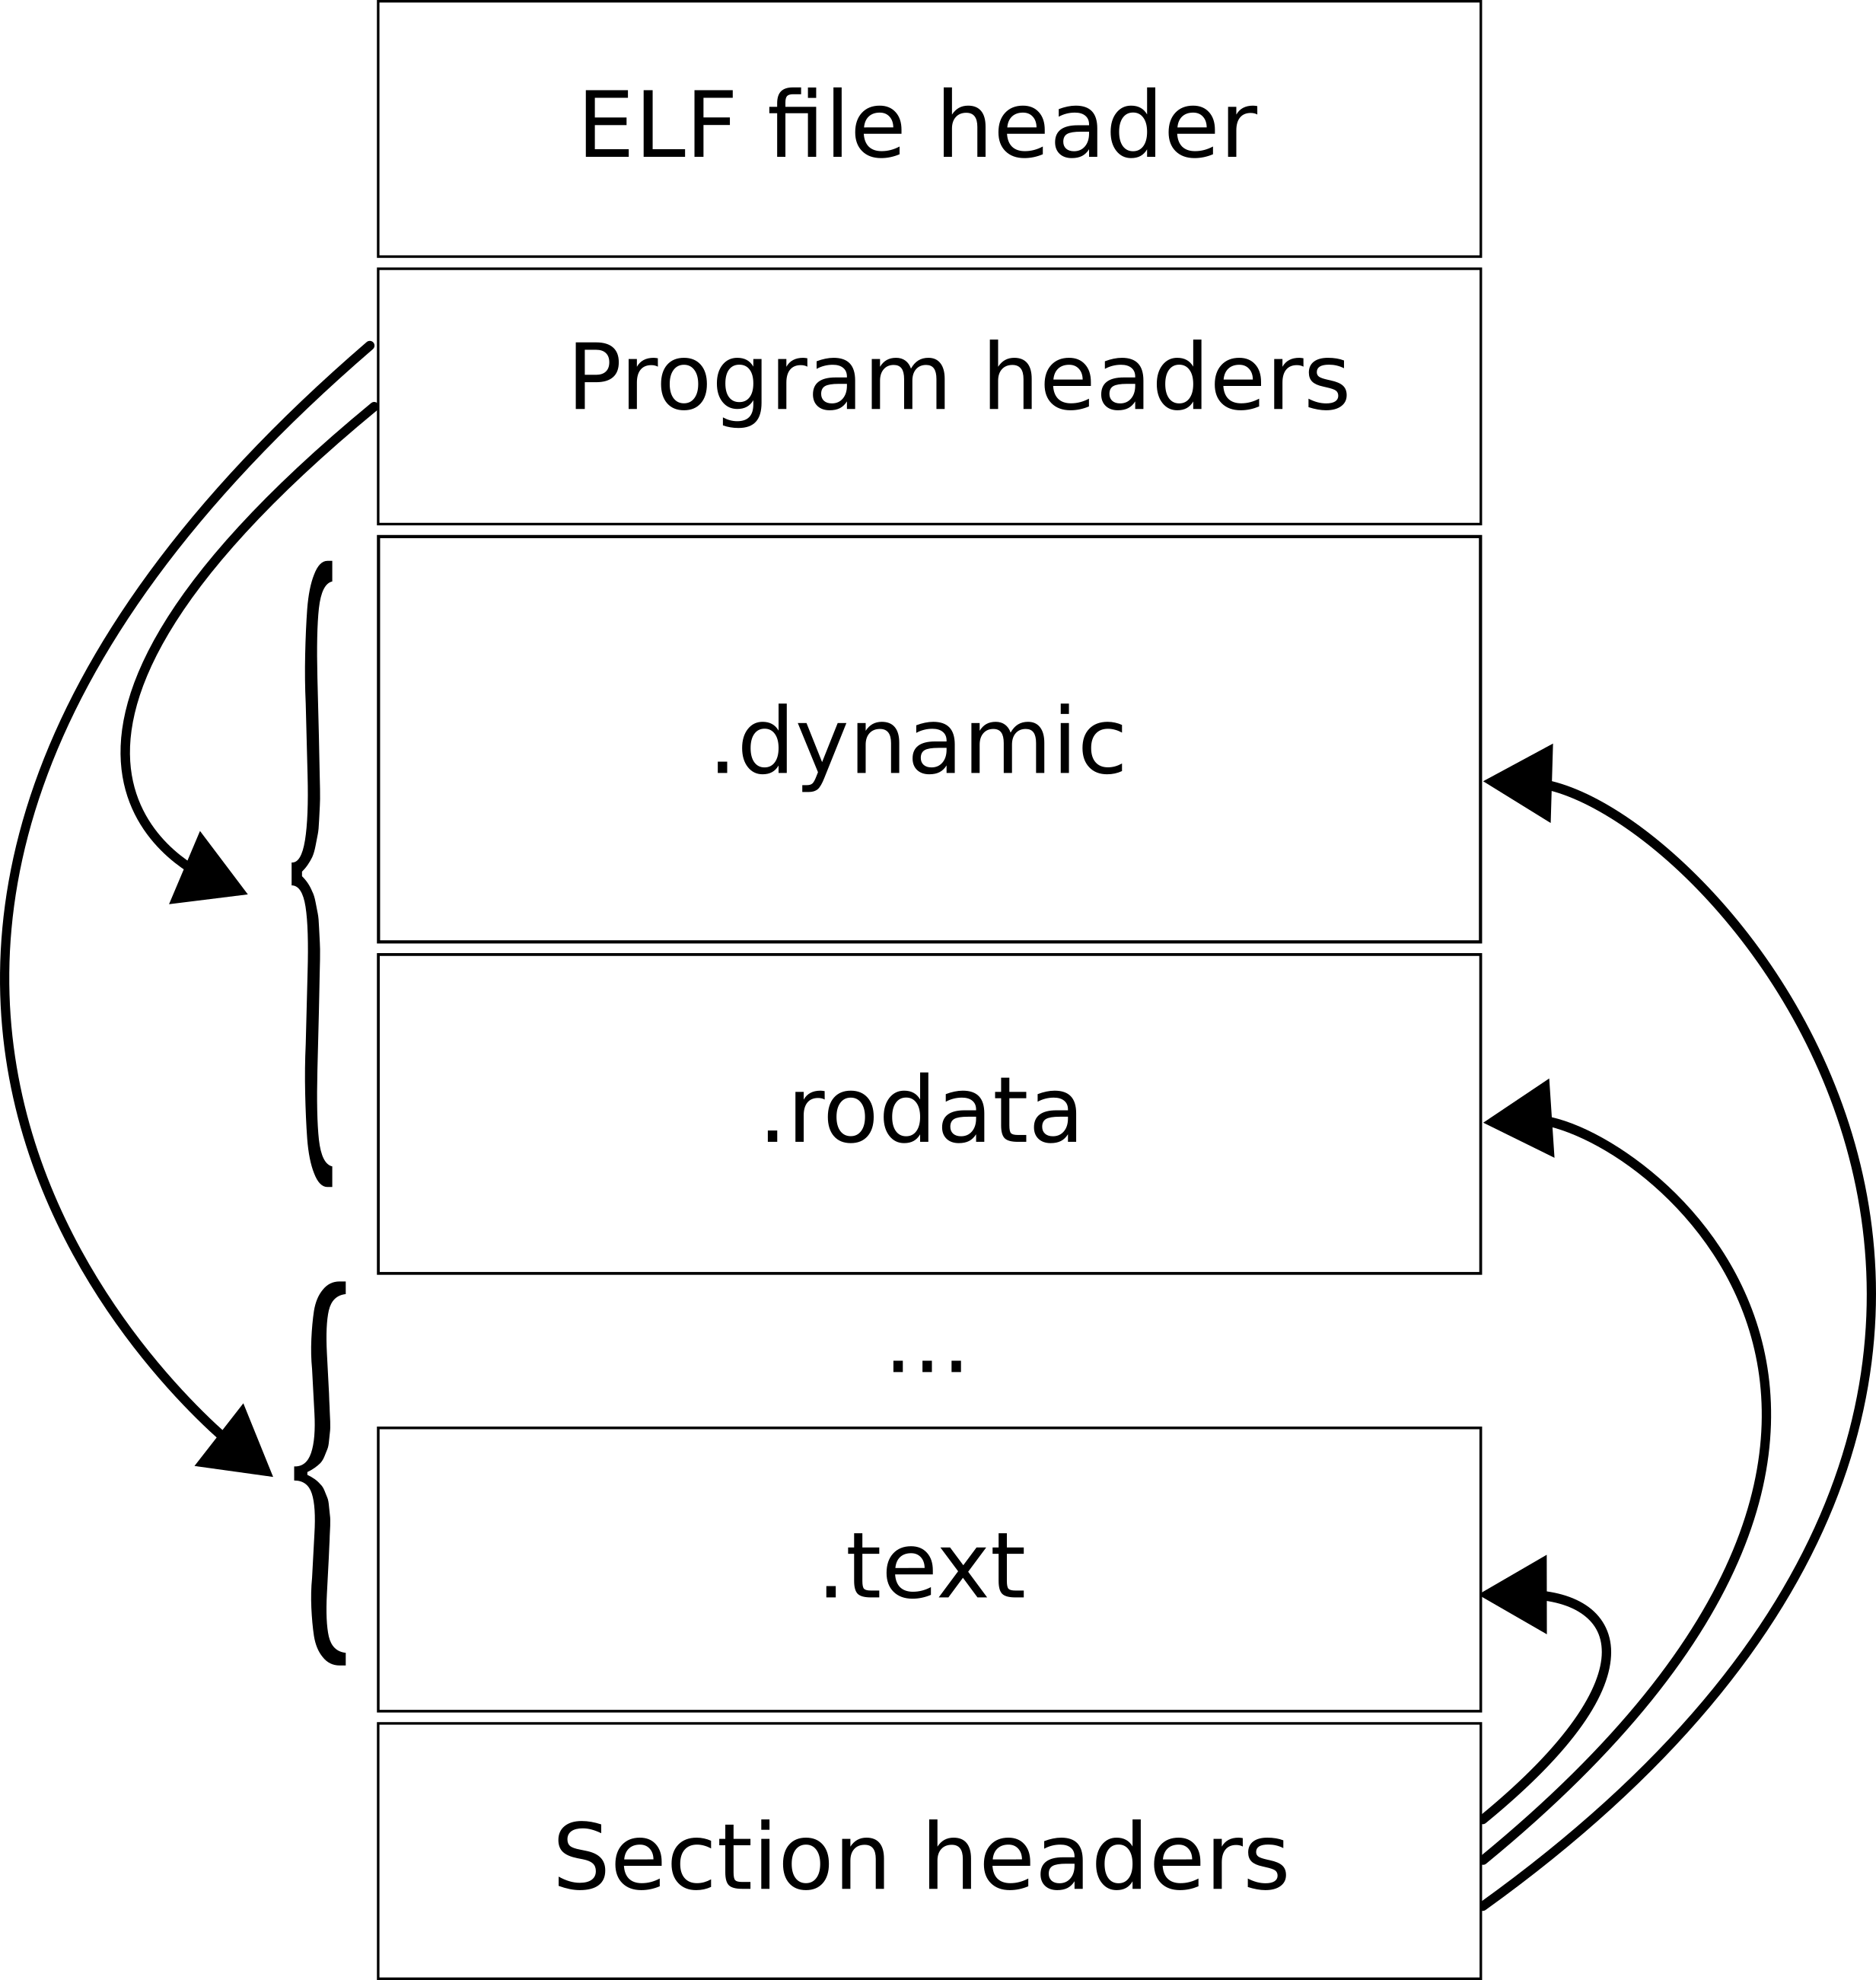
\includegraphics[width=0.5\textwidth]{inc/2_lit_review/elf_file_structure.png}
		\caption{The basic structure of an ELF file.\protect\footnotemark}
		\label{fig:elf_file_structure}
	\end{center}
\end{figure}
\footnotetext{Original image (CC BY-SA): \url{https://en.wikipedia.org/wiki/File:Elf-layout--en.svg}}

All ELF files starts with the four byte identifier \texttt{0x7F}, \texttt{'E'}, \texttt{'L'}, \texttt{'F'} which marks the beginning of the ELF file header. The ELF file header contains general information about a binary, such as its object file type (executable, relocatable or shared object), its assembly architecture (x86-64, ARM, …), the virtual address of its entry point which indicates the starting point of program execution, and the file offsets to the program and section headers.

Each program and section header describes a continuous segment or section of memory respectively. In general, segments are used by the linker to load executables into memory with correct access permissions, while sections are used by the compiler to categorize data and instructions. Therefore, the program headers are optional for relocatable and shared objects, while the section headers are optional for executables.

\begin{figure}[htbp]
	\begin{center}
		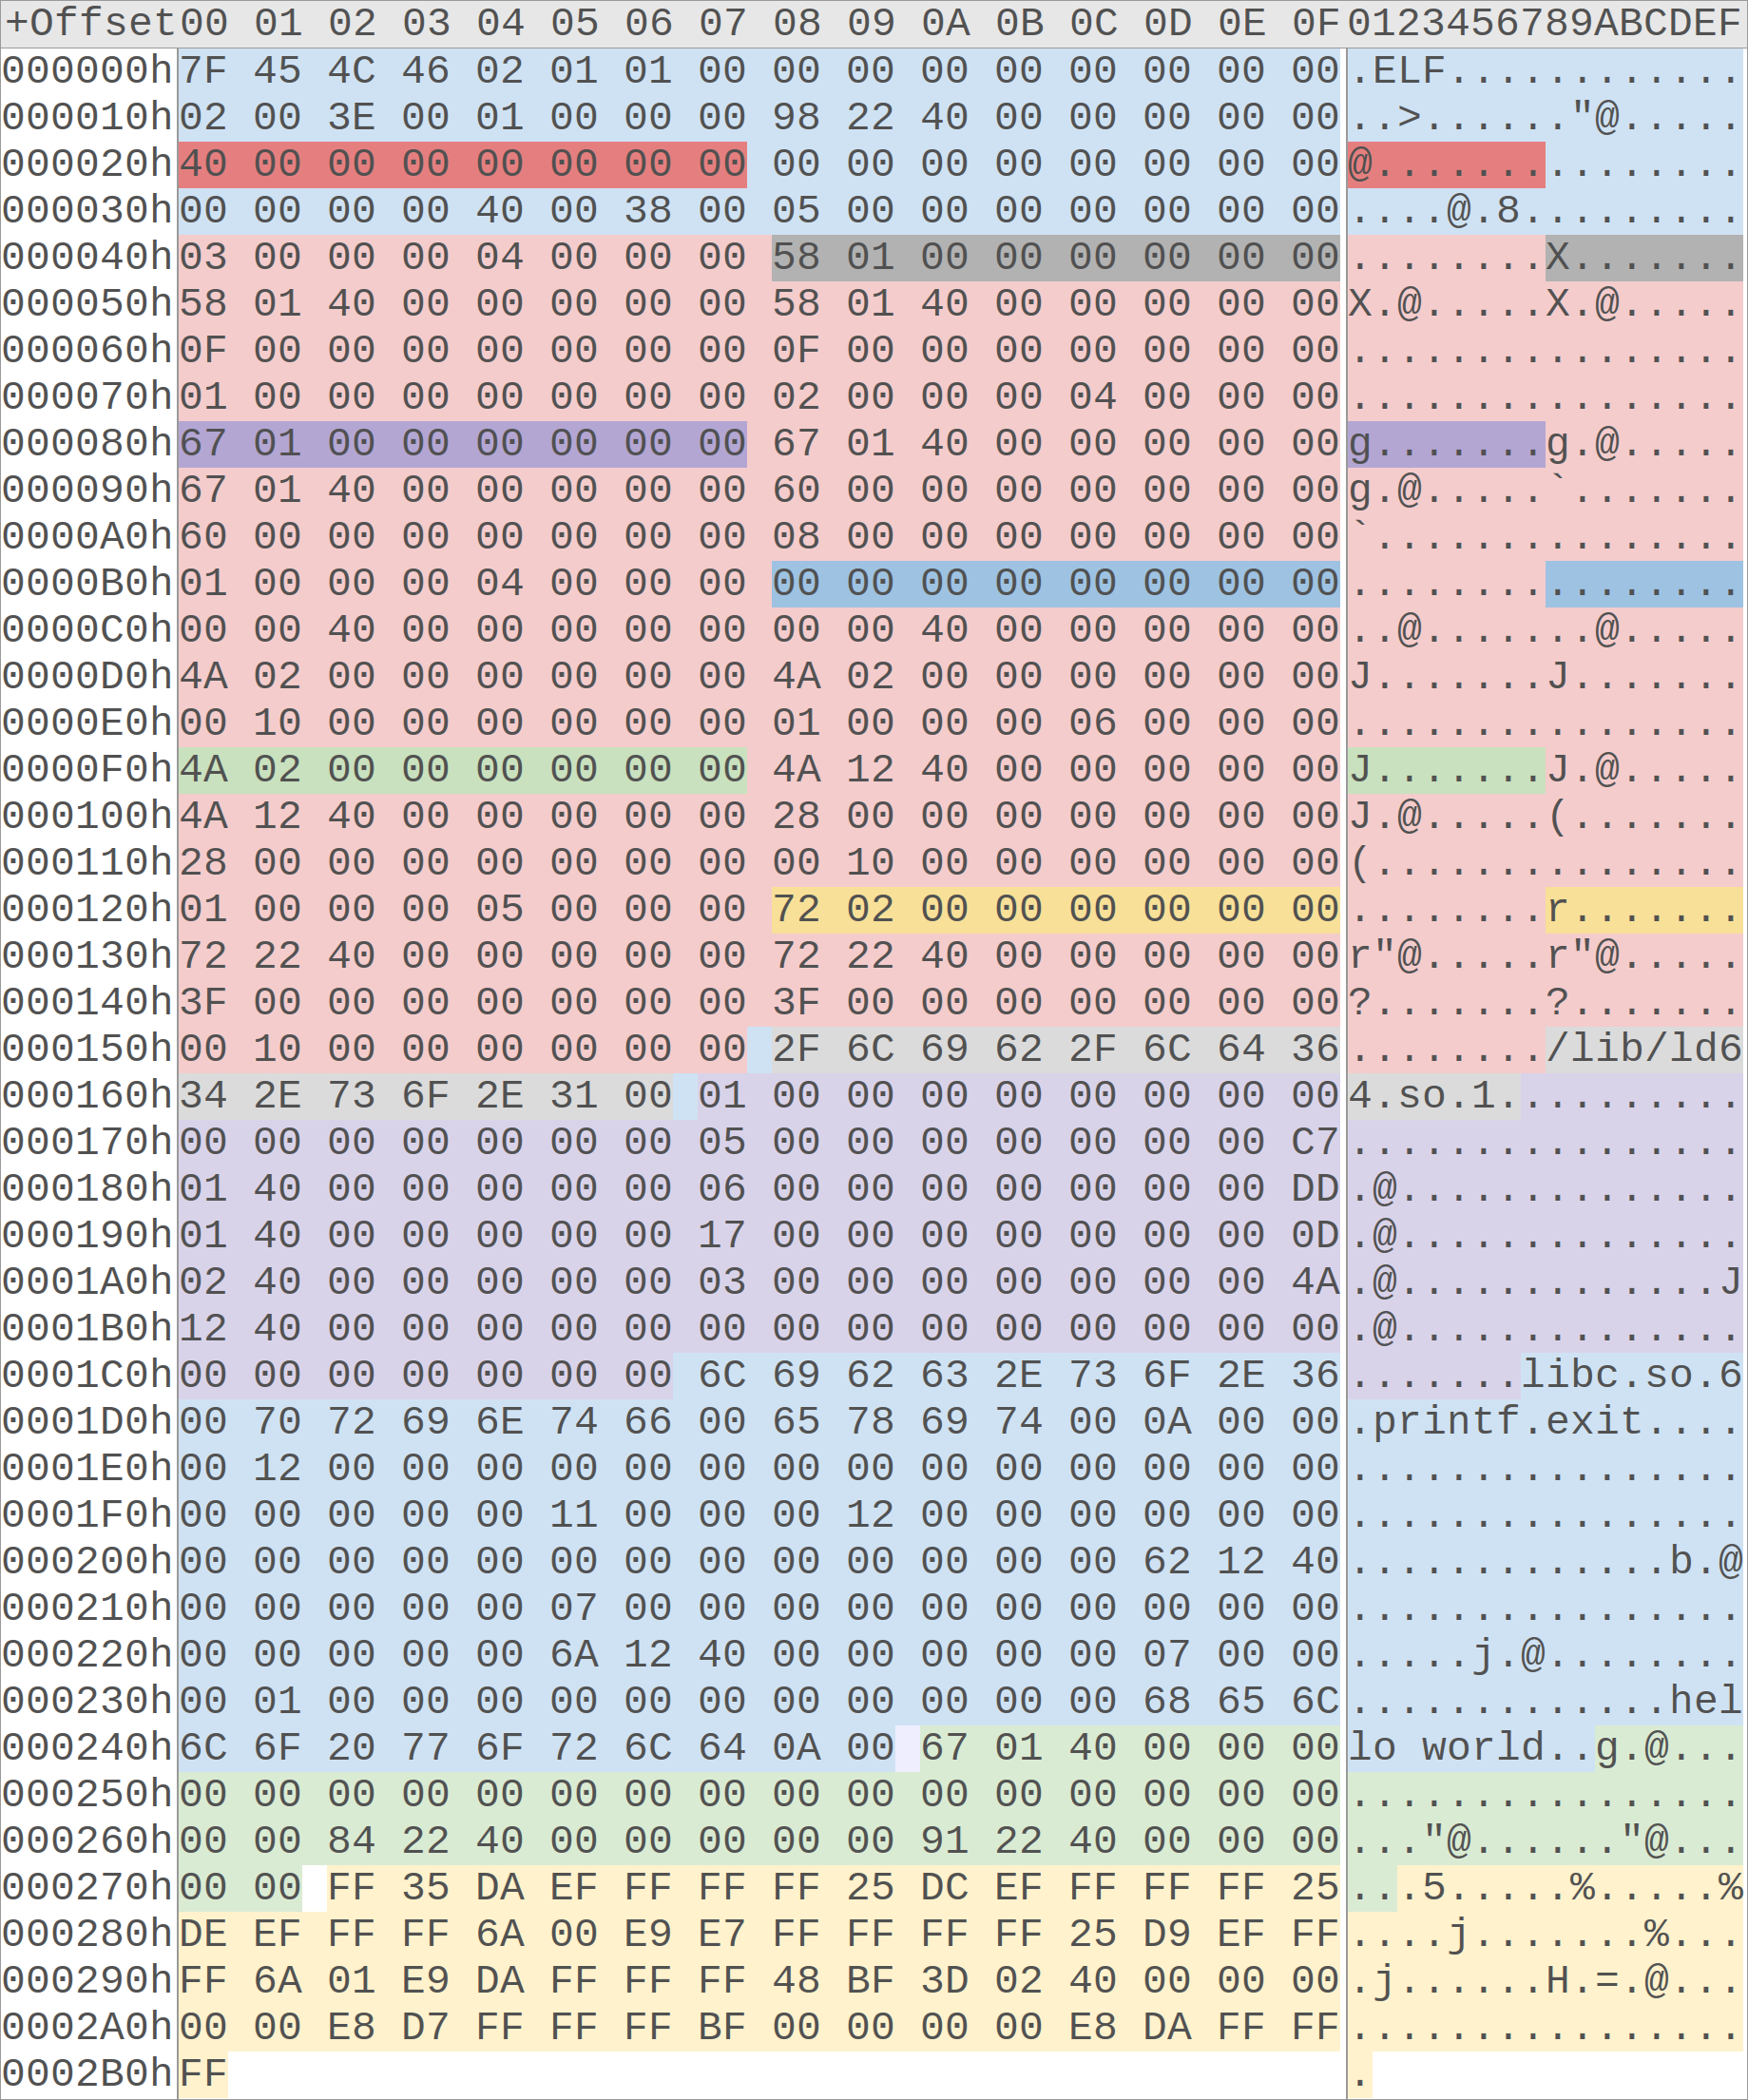
\includegraphics[width=\textwidth]{inc/2_lit_review/elf_dissection.png}
		\caption{The entire contents of a simple \textit{``hello world''} ELF executable with colour-coded file offsets, sections, segments and program headers. Each file offset is 8 bytes in width and coloured using a darker shade of its corresponding segment, section or program header.}
		\label{fig:elf_dissection}
	\end{center}
\end{figure}

To further investigate the structure of ELF files a simple 64-bit \textit{``hello world''} executable has been dissected and its content colour-coded. Each file offset of the executable consists of 8 bytes and is denoted in figure \ref{fig:elf_dissection} with a darker shade of the colour used by its corresponding target segment, section or program header. Starting at the middle of the ELF file header, at offset \texttt{0x20}, is the file offset (red) to the program table (bright red). The program table contains five program headers which specify the size and file offsets of two sections and three segments, namely the \texttt{.interp} (grey) and the \texttt{.dynamic} (purple) sections, and a \textit{read-only} (blue), a \textit{read-write} (green) and a \textit{read-execute} (yellow) segment.

Several sections are contained within the three segments. The \textit{read-only} segment contains the following sections:

\begin{itemize}
	\item \texttt{.interp}: the interpreter, i.e. the linker
	\item \texttt{.dynamic}: array of dynamic entities
	\item \texttt{.dynstr}: dynamic string table
	\item \texttt{.dynsym}: dynamic symbol table
	\item \texttt{.rela.plt}: relocation entities of the PLT
	\item \texttt{.rodata}: read-only data section
\end{itemize}

The \textit{read-write} segment contains the following section:

\begin{itemize}
	\item \texttt{.got.plt}: Global Offset Table (GOT) of the PLT (henceforth referred to as the GOT as this executable only contains one such table)
\end{itemize}

And the \textit{read-execute} segment contains the following sections:

\begin{itemize}
	\item \texttt{.plt}: Procedure Linkage Table (PLT)
	\item \texttt{.text}: executable code section
\end{itemize}

Seven of the nine sections contained within the executable are directly related to dynamic linking. The \texttt{.interp} section specifies the linker (in this case \textit{``/lib/ld64.so.1''}) and the \texttt{.dynamic} section an array of dynamic entities containing offsets and virtual addresses to relevant dynamic linking information. In this case the dynamic array specifies that \textit{``libc.so.6''} is a required library, and contains the virtual addresses to the \texttt{.dynstr}, \texttt{.dynsym}, \texttt{.rela.plt} and \texttt{.got.plt} sections. As noted, even a simple \textit{``hello world''} executable requires a large number of sections related to dynamic linking. Further analysis will reveal their relation to each other and describe their usage.

The dynamic string table contains the names of libraries (e.g. \textit{``libc.so.6''}) and identifiers (e.g. \textit{``printf''}) which are required for dynamic linking. Other sections refer to these strings using offsets into \texttt{.dynstr}. The dynamic symbol table declares an array of dynamic symbol entities, each specifying the name (e.g. offset to \textit{``printf''} in \texttt{.dynstr}) and binding information (local or global) of a dynamic symbol. Both the \texttt{.plt} and the \texttt{.rela.plt} sections refers to these dynamic symbols using array indicies. The \texttt{.rela.plt} section specifies the relocation entities of the PLT; more specifically this section informs the linker of the virtual address to the \texttt{.printf} and \texttt{.exit} entities in the GOT.

To reflect on how dynamic linking is accomplished on a Linux system lets review the assembly instructions of the executable \texttt{.text} and \texttt{.plt} sections as outlined in listing \ref{lst:elf_text} and \ref{lst:elf_plt} respectively.

\lstinputlisting[language=nasm, style=nasm, caption={The assembly instructions of the \texttt{.text} section. \label{lst:elf_text}}]{inc/2_lit_review/elf_text.asm}

\lstinputlisting[language=nasm, style=nasm, caption={The assembly instructions of the \texttt{.plt} section. \label{lst:elf_plt}}]{inc/2_lit_review/elf_plt.asm}

As visualised in listing \ref{lst:elf_text} the first call instruction of the \texttt{.text} section targets the \texttt{.printf} label of the \texttt{.plt} section instead of the actual address of the \textit{printf} function in the \textit{libc} library. The Procedure Linkage Table (PLT) provides a level of indirection between call instructions and actual function (procedure) addresses, and contains one entity per external function as outlined in listing \ref{lst:elf_plt}. The \texttt{.printf} entity of the PLT contains a jump instruction which targets the address stored in the \texttt{.printf} entity of the GOT. Initially this address points to the next instruction, i.e. the instruction denoted by the \texttt{.resolve\_printf} label in the PLT. On the first invokation of \textit{printf} the linker replaces this address with the actual address of the \textit{printf} function in the \textit{libc} library, and any subsequent invokation of \textit{printf} will target the resolved function address directly.

This method of external function resolution is called lazy dynamic linking as it postpones the work and only resolves a function once it is actually invoked at runtime. The lazy approach to dynamic linking may improve performance by limiting the number of symbols that require resolution. At the same time the eager approach may benefit latency sensitive applications which cannot afford the cost of dynamic linking at runtime.

A closer look at the instructions denoted by the \texttt{.resolve\_printf} label in listing \ref{lst:elf_plt} reveals how the linker knows which function to resolve. Essentially the \textit{dl\_runtime\_resolve} function is invoked with two arguments, namely the dynamic symbol index of the \textit{printf} function and a pointer to a linked list of nodes, each refering to the \texttt{.dynamic} section of a shared object. Upon termination the linked list of our \textit{``hello world''} process contains a total of four nodes, one for the executable itself and three for its dynamically loaded libraries, namely \textit{linux-vdso.so.1}, \textit{libc.so.6} and \textit{ld64.so.1}.

To summarise, the execution of a dynamically linked executable can roughly be described as follows. Upon execution the kernel parses the program headers of the ELF file, maps each segment to one or more pages in memory with appropriate access permissions, and transfers the control of execution to the linker (\textit{``/lib/ld64.so.1''}) which was loaded in a similar fashion. The linker is responsible for initiating the addresses of the \textit{dl\_runtime\_resolve} function and the aforementioned linked list, both of which are stored in the GOT of the executable. After this setup is complete the linker transfers control to the entry point of the executable, as specified by the ELF file header (in this case the \texttt{.start} label of the \texttt{.text} section). At this point the assembly instructions of the application are executed until termination and external functions are lazily resolved at runtime by the linker through invocations to the \textit{dl\_runtime\_resolve} function.

% --- [ Decompilation Phases ] -------------------------------------------------

\subsection{Decompilation Phases}
\label{sec:lit_review_decompilation_phases}

A core principle utilized in decompilers is the separation of concern through the use of abstractions, and extensive work involves translating into and breaking out of various abstraction layers. In general, a decompiler is composed of distinct phases which parse, analyse or transform the input. These phases are conceptually grouped into three modules to separate concerns regarding source machine language and target programming language. Firstly, the front-end module parses executable files and translates their platform-dependent assembly into a platform-independent intermediate representation (IR). Secondly, the middle-end module performs a set of decompilation passes to lift the IR, from a low-level to a high-level representation, by reconstructing high-level control structures and expressions. Lastly, the back-end module translates the high-level IR to a specific target programming language \cite{reverse_comp}. Figure \ref{fig:modules_overview} gives an overview of the decompilation modules and visualises their relationship.

\begin{figure}[htbp]
	\begin{center}
		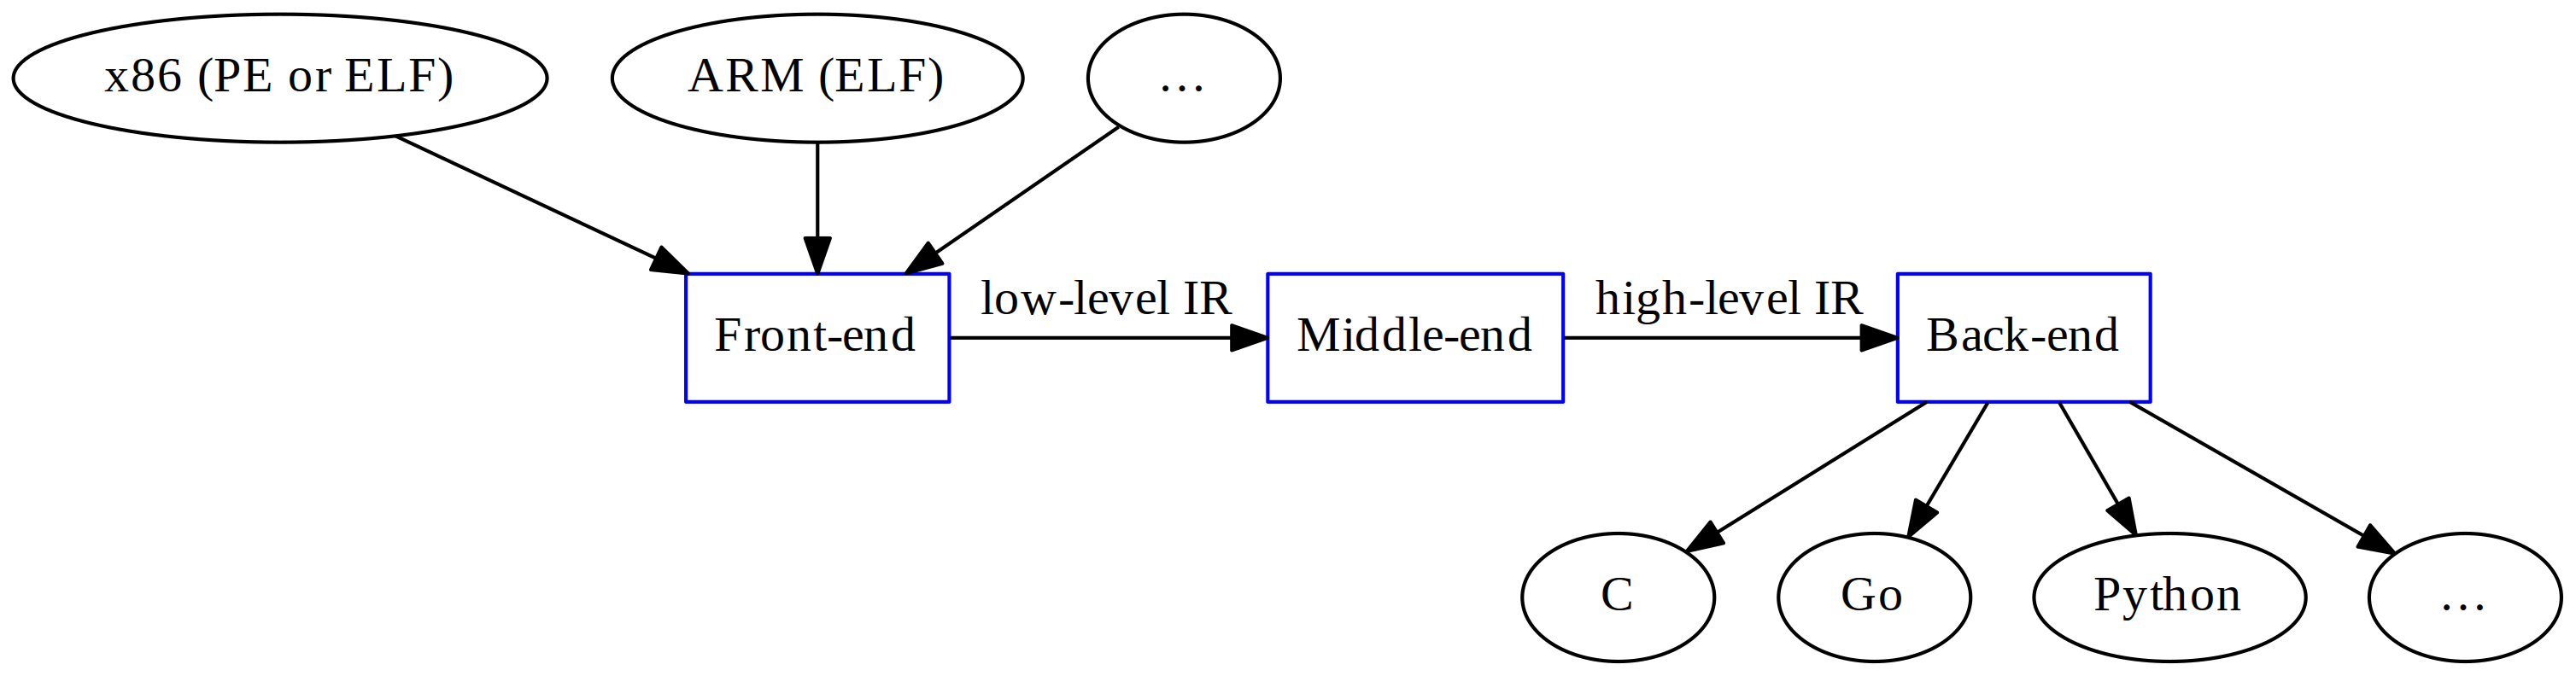
\includegraphics[width=\textwidth]{inc/2_lit_review/modules_overview.png}
		\caption{Firstly, the front-end module accepts several executable file formats (PE, ELF, …) as input and translates their platform-dependent assembly (x86, ARM, …) to a low-level IR. Secondly, the middle-end module lifts the low-level IR to a high-level IR through a set of decompilation passes. Lastly, the back-end module translates the high-level IR into one of several target programming languages (C, Go, Python, …).}
		\label{fig:modules_overview}
	\end{center}
\end{figure}

The remainder of this section describes the distinct decompilation phases, most of which have been thoroughly described by Cristina Cifuentes in her influential paper \textit{``Reverse Compilation Techniques''} \cite{reverse_comp}.

% --- [ Subsubsections ] -------------------------------------------------------

% ~~~ [ Binary Analysis ] ~~~~~~~~~~~~~~~~~~~~~~~~~~~~~~~~~~~~~~~~~~~~~~~~~~~~~~

\subsubsection{Binary Analysis}
\label{sec:lit_review_binary_analysis}

As demonstrated in section \ref{sec:lit_review_the_anatomy_of_an_executable}, parsing even a simple \textit{``hello world''} executable requires extensive knowledge of its binary file format (in this case ELF). The binary analysis phase is responsible for parsing input files of various binary file formats, such as PE and ELF, and present their content in a uniform manner which preserves the relations between file contents, virtual addresses and access permissions. Later stages of the decompilation pipeline builds upon this abstraction to access the file contents of each segment or section without worrying about the details of the underlying file format. Information about external symbols, metadata and the computer architecture of the assembly may also be provided by this abstraction.

% ~~~ [ Disassembly ] ~~~~~~~~~~~~~~~~~~~~~~~~~~~~~~~~~~~~~~~~~~~~~~~~~~~~~~~~~~

\subsubsection{Disassembly}

The disassembly phase (referred to as the \textit{syntactic analysis phase} by C. Cifuentes) is responsible for decoding the raw machine instructions of the executable segments into assembly. The computer architecture dictates how the assembly instructions and their associated operands are encoded. Generally CISC architectures (e.g. x86) use variable length instruction encoding (e.g. instructions occupy between 1 and 17 bytes in x86) and allow memory addressing modes for most instructions (e.g. arithmetic instructions may refer to memory locations in x86) \cite{x86_manual}. In contract, RISC architectures (e.g. ARM) generally use fixed-length instruction encoding (e.g. instructions always occupy 4 bytes in AArch64) and only allow memory access through load-store instructions (e.g. arithmetic instructions may only refer to registers or immediate values in ARM) \cite{arm_manual}.

One of the main problems of the disassembly phase is how to separate code from data. In the Von Neumann architecture the same memory unit may contain both code and data. Furthermore, the data stored in a given memory location may be interpreted as code by one part of the program, and as data by another part. In contrast, the Harvard architecture uses separate memory units for code and data \cite{von_neumann_vs_harvard}. Since the use of the Von Neumann architecture is wide spread, solving this problem is fundamental for successful disassemblers.

% TODO: Add switch tables example.

A solution to the problem of separating code from data is to use recursive descent instead of linear descent when parsing assembly instructions.

% TODO: Add description of recursive descent and linear descent.

\begin{figure}[htbp]
	\centering
	\begin{subfigure}[t]{0.49\textwidth}
		\lstinputlisting[language=nasm, style=nasm, tabsize=2]{inc/hello/hello_linear.asm}
		\caption{Disassembly from \texttt{objdump} and \texttt{ndisasm}\protect\footnotemark.}
	\end{subfigure}
	\qquad
	\begin{subfigure}[t]{0.35\textwidth}
		\lstinputlisting[language=nasm, style=nasm, tabsize=2]{inc/hello/hello_recursive.asm}
		\caption{Disassembly from IDA Pro.}
	\end{subfigure}
	\caption{The disassembly produced by a linear descent parser (left) and a recursive descent parser (right) when analyzing a simple \textit{``hello world''} program that stores the \texttt{hello} string in the executable segment.}
\end{figure}
\footnotetext{The Netwide Disassembler: \url{http://www.nasm.us/doc/nasmdoca.html}}

One problem faced by both linear descent and recursive descent disassemblers is the need for a starting point. In practise, exported entry point symbols (e.g. \texttt{main}, \texttt{start}, \texttt{DLLMain}, …) works well.

% TODO: Verify that it is called symbolic execution/symbolic execution engine.

Another problem for recursive descent disassemblers is indirect branches (e.g. jump to the address stored in a register). In the case of indirect branches, it is impossible to know the branch target by only looking at the individual instructions. One solution is to use symbolic execution, which emulates the processor and executes instructions to give information about the value stored in registers. With this method the target of indirect jumps may be calculated. There are problems to consider when designing a symbolic execution engine, for instance the impact of cached memory access. See figure \ref{foo} for an example of where cache details matter for the execution flow.

% TODO: Add example where the cache impacts execution flow (pipeline pre-schedules). *addr = 5; jmp addr

% Problems:
% * self-modifying code
% * Architecture-dependent Restrictions
%    Cannot be determined by step-by-step debugging; as the prefetch pipeline
%    would behave differently.
%       mov ax, 0x9090
%       mov [jmpDef], ax
%    jmpDef:
%       jmp codeExecuted
%    codeNotExecuted:
%       foo
%    codeExecuted:
%       bar

Another issue is the use of callbacks, which is common in GUI applications.
% TODO: Solution? Run program and use breakpoints?

There exists several anti-disassembly techniques which are commonly used by malware. One such technique exploits the fact that recursive descent parsers follow both the true and the false branch of conditional branch instructions, as demonstrated in figure \ref{fig:anti-disassembly}.

The recursive descent parser cannot parse both the false and the true-branch of the conditional branch instruction at line 3, because the true branch targets the middle of a \texttt{jmp} instruction.

The conditional branch instruction at line 3 always takes the true branch, which points to the middle of the \texttt{jmp} instruction decoded when parsing the false branch. The recursive descent parser cannot disassembly both branches and is forced to choose one of them, in this case the \texttt{fake} branch.

The recursive descent parser fails by using a conditional branch instruction (\texttt{jz}) which always takes the true-branches \texttt{fake+1} which is in the middle of an instruction.

\begin{figure}[htbp]
	\centering
	\begin{subfigure}[t]{0.59\textwidth}
		\lstinputlisting[language=nasm, style=nasm, tabsize=2]{inc/hello/anti_orig.asm}
		\caption{Original assembly.}
	\end{subfigure}
	\qquad
	\begin{subfigure}[t]{0.34\textwidth}
		\lstinputlisting[language=nasm, style=nasm, tabsize=2]{inc/hello/anti_fail.asm}
		\caption{Disassembly from IDA Pro.}
	\end{subfigure}
	\caption{The original assembly (left) contains an anti-disassembly trick which causes the recursive descent parser to fail (right).}
	\label{fig:anti-disassembly}
\end{figure}

The anti-disassembly technique presented in figure \ref{fig:anti-disassembly} may be mitigated using symbolic execution, which could verify that the conditional jump always takes the true branch and therefore allow the instruction to be replaced with an unconditional jump to the target of the true branch. This quickly becomes a game of cat-and-mouse, as the anti-disassembly techniques could be extended to rely on network activity, file contents, or other external sources which would render the symbolic exeuction useless.

To conclude, the disassembly phase deals with non-trivial problems, some of which are difficult to automate. Advanced disassemblers therefore provide interactive capabilities and rely on human intuition to solve ambiguities and direct the disassembler out of corner cases. See section \ref{sec:related_work_hex-rays_decompiler} for further details on such disassemblers.

% TODO: Introduce the various approaches and highlight their individual
% strengths and weaknesses.
%
% NAIVE APPROACH: linear descent disassemblers.
% PROBLEM: Highlight problems with linear descent disassemblers.
%    - rodata (e.g. "hello world") and jump tables in code.
%
% SOLUTION: recursive descent disassemblers.
% PROBLEM: Highlight problems with recursive descent disassemblers.
%    - Distinguish between code and data (e.g. find entry points of functions).
%      Not add functions are directly referred to (e.g. callback functions which
%      are commonly used by GUI applications).
%    - Easy to fool.
%       xor eax, eax
%       cmp eax, 0
%       jz foo+1 ; Cannot disassembly both foo and foo+1.
% foo:
%       add eax, 3
%
% SOLUTION: symbolic execution engines.
% PROBLEM: security, performance, ...?

% ~~~ [ Control Flow Analysis ] ~~~~~~~~~~~~~~~~~~~~~~~~~~~~~~~~~~~~~~~~~~~~~~~~

\subsubsection{Control Flow Analysis}
\label{sec:lit_review_control_flow_analysis}

The control flow analysis stage is responsible for analysing the control flow (i.e. flow of execution) of source programs to recover their high-level control flow structures. The control flow of a given function is determined by its branching instructions and may be expressed as a control flow graph (CFG), which is a connected graph with a single entry node (the function entry point) and zero or more exit nodes (the function return statements). A key insight provided by C. Cifuentes and S. Moll is that high-level control flow primitives (such as 1-way conditionals and pre-test loops) may be expressed using graph representations \cite{reverse_comp, decomp_of_llvm}, as illustrated in figure \ref{fig:graph_representations}. The problem of recovering high-level control flow primitives from CFGs may therefore be reformulated as the problem of identifying subgraphs (i.e. the graph representation of a high-level control flow primitive) in graphs (i.e. the CFG of a function) without considering node names. This problem is commonly referred to as \textit{subgraph isomorphism search}, the general problem of which is NP-hard \cite{subgraph_isomorphism_algorithms}. However, the problem which is required to be solved by the control flow analysis stage may be simplified by exploiting known properties of CFGs (e.g. connected graph with a single entry node).

\begin{figure}[htbp]
	\centering
	% if
	\begin{subfigure}[ht]{0.23\textwidth}
		\centering
		\begin{subfigure}[ht]{0.45\textwidth}
			\lstinputlisting[language=go, style=go, breaklines=false, numbers=none]{inc/primitives/if.c}
		\end{subfigure}
		\begin{subfigure}[ht]{0.42\textwidth}
			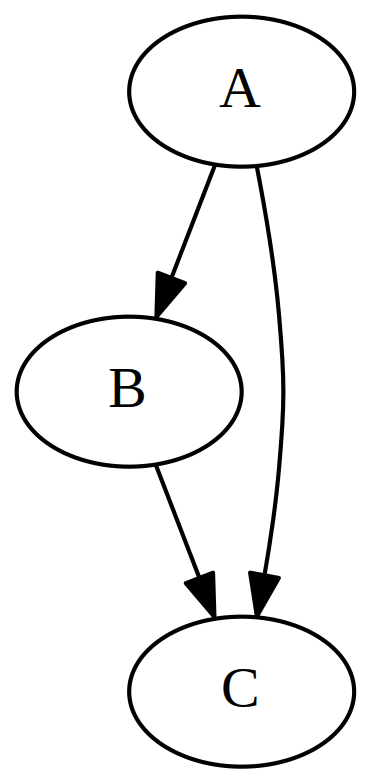
\includegraphics[width=\textwidth]{inc/primitives/if.png}
		\end{subfigure}
		\caption{1-way conditional; entry: \texttt{A}, exit: \texttt{C}.}
		\label{fig:if_graph_representation}
	\end{subfigure}
	\qquad
	% if_else
	\begin{subfigure}[ht]{0.28\textwidth}
		\centering
		\begin{subfigure}[ht]{0.45\textwidth}
			\lstinputlisting[language=go, style=go, breaklines=false, numbers=none]{inc/primitives/if_else.c}
		\end{subfigure}
		\begin{subfigure}[ht]{0.50\textwidth}
			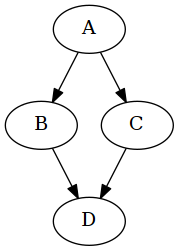
\includegraphics[width=\textwidth]{inc/primitives/if_else.png}
		\end{subfigure}
		\caption{2-way conditional; entry: \texttt{A}, exit: \texttt{D}.}
		\label{fig:if_else_graph_representation}
	\end{subfigure}
	\qquad
	% if_return
	\begin{subfigure}[ht]{0.30\textwidth}
		\centering
		\begin{subfigure}[ht]{0.45\textwidth}
			\lstinputlisting[language=go, style=go, breaklines=false, numbers=none]{inc/primitives/if_return.c}
		\end{subfigure}
		\begin{subfigure}[ht]{0.50\textwidth}
			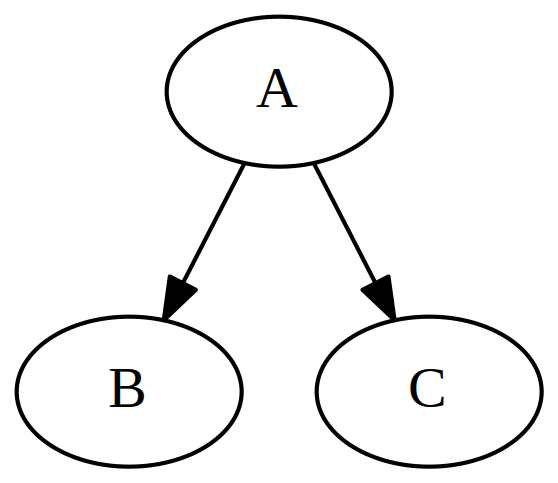
\includegraphics[width=\textwidth]{inc/primitives/if_return.png}
		\end{subfigure}
		\caption{1-way condition with return statement in body; entry: \texttt{A}, exit: \texttt{C}.}
		\label{fig:if_return_graph_representation}
	\end{subfigure}
	\qquad
	% pre_loop
	\begin{subfigure}[ht]{0.32\textwidth}
		\centering
		\begin{subfigure}[ht]{0.45\textwidth}
			\lstinputlisting[language=C, style=go, breaklines=false, numbers=none]{inc/primitives/pre_loop.c}
		\end{subfigure}
		\begin{subfigure}[ht]{0.50\textwidth}
			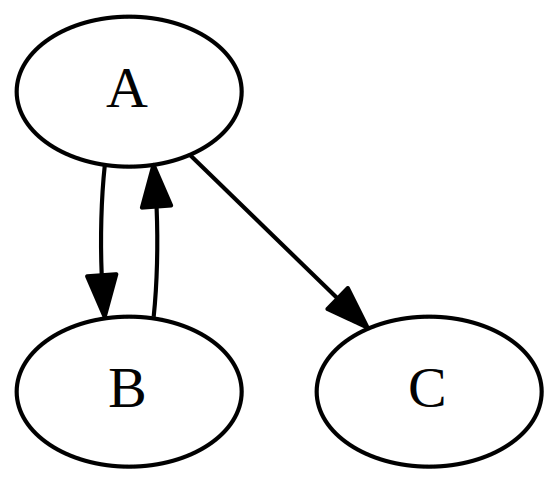
\includegraphics[width=\textwidth]{inc/primitives/pre_loop.png}
		\end{subfigure}
		\caption{pre-test loop; entry: \texttt{A}, exit: \texttt{C}.}
		\label{fig:pre_loop_graph_representation}
	\end{subfigure}
	\qquad
	% post_loop
	\begin{subfigure}[ht]{0.30\textwidth}
		\centering
		\begin{subfigure}[ht]{0.50\textwidth}
			\lstinputlisting[language=C, style=go, breaklines=false, numbers=none]{inc/primitives/post_loop.c}
		\end{subfigure}
		\begin{subfigure}[ht]{0.35\textwidth}
			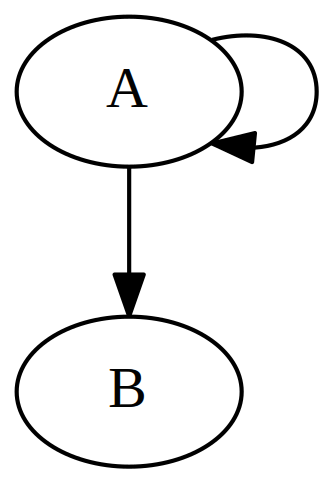
\includegraphics[width=\textwidth]{inc/primitives/post_loop.png}
		\end{subfigure}
		\caption{post-test loop; entry: \texttt{A}, exit: \texttt{B}.}
		\label{fig:post_loop_graph_representation}
	\end{subfigure}
	\qquad
	% list
	\begin{subfigure}[ht]{0.24\textwidth}
		\centering
		\begin{subfigure}[ht]{0.20\textwidth}
			\lstinputlisting[language=C, style=go, breaklines=false, numbers=none]{inc/primitives/list.c}
		\end{subfigure}
		\begin{subfigure}[ht]{0.35\textwidth}
			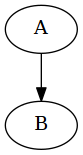
\includegraphics[width=\textwidth]{inc/primitives/list.png}
		\end{subfigure}
		\caption{consecutive statements; entry: \texttt{A}, exit: \texttt{B}.}
		\label{fig:list_graph_representation}
	\end{subfigure}
	\caption{The pseudo-code and graph representation of various high-level control flow primitives with denoted entry and exit nodes.}
	\label{fig:graph_representations}
\end{figure}

When the subgraph isomorphism of a high-level control flow primitive has been identified in the CFG of a function, it may be replaced by a single node that inherits the predecessors of the subgraph entry node and the successors of the subgraph exit node; as illustrated in figure \ref{fig:subgraph_merge}. By recording the node names of the identified subgraphs and the name of their corresponding high-level control flow primitives, the high-level control flow structure of a CFG may be recovered by successively identifying subgraph isomorphisms and replacing them with single nodes until the entire CFG has been reduced into a single node; as demonstrated by the step-by-step simplification of a CFG in appendix \ref{app:control_flow_analysis_example}. Should the control flow analysis fail to reduce a CFG into a single node, the CFG is considered irreducible with regards to the supported high-level control flow primitives (see figure \ref{fig:graph_representations}). To structure arbitrary irreducible graphs, S. Moll applied node splitting (which translates irreducible graphs into reducible graphs by duplicating nodes) to produce functionally equivalent target programs \cite{decomp_of_llvm}. In contrast, C. Cifuentes focused on preserving the structural semantics of the source program (which may be required in forensics investigations), and therefore used \texttt{goto}-statements in these cases to produce unstructured target programs.

\begin{figure}[htbp]
	\centering
	\begin{subfigure}[ht]{0.15\textwidth}
		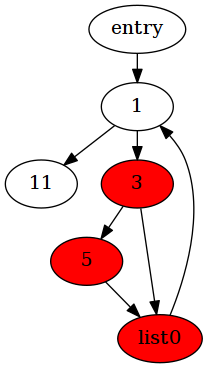
\includegraphics[width=\textwidth]{inc/2_lit_review/cfg_pre_merge.png}
	\end{subfigure}
	\qquad
	\begin{subfigure}[ht]{0.15\textwidth}
		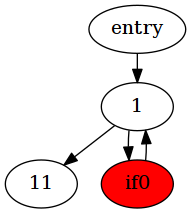
\includegraphics[width=\textwidth]{inc/2_lit_review/cfg_post_merge.png}
	\end{subfigure}
	\caption{The left side illustrates the CFG of a function in which the graph representation of a 1-way conditional (see figure \ref{fig:if_graph_representation}) has been identified, and the right side illustrates the same CFG after the subgraph has been replaced with a single node (i.e. \texttt{if0}) that inherits the predecessors of the subgraph entry node (i.e. \texttt{3}) and the successors of the subgraph exit node (i.e. \texttt{list0}).}
	\label{fig:subgraph_merge}
\end{figure}


% --- [ Evaluation of Intermediate Representations ] ---------------------------

\subsection{Evaluation of Intermediate Representations}

Decompilers face similar problems as both binary analysis tools and compilers. Therefore, it seems reasonable that the intermediate representations (IRs) used in these domains may be well suited for decompilation purposes. This section evaluates one IR from each domain with regards to their suitability for recovering high-level control flow primitives (objective \ref{itm:obj_control_flow_analysis_component}) and expressions (objective \ref{itm:obj_data_analysis_library}).

% ~~~ [ REIL ] ~~~~~~~~~~~~~~~~~~~~~~~~~~~~~~~~~~~~~~~~~~~~~~~~~~~~~~~~~~~~~~~~~

\subsubsection{REIL}

The Reverse Engineering Intermediate Language (REIL) is a very simple and platform independent assembly language. The REIL instruction set contains only 17 different instructions, each with exactly three (possibly empty) operands. The first two operands are always used for input and the third for output (except for the conditional jump instruction which uses the third operand as the jump target). Furthermore, each instruction has at most one effect on the global state and never any side-effects (such as setting flags) \cite{reil_paper,reil_spec}. Thanks to the simplicity of REIL a full definition of its instruction set has been provided in appendix \ref{app:reil_instructions}, which includes examples of each instruction and defines their syntax and semantics (in pseudo C-code).

When translating native assembly (e.g. x86) into REIL, the original addresses of each instruction is left shifted by 8 bits to allow 256 REIL instructions per address. Each native instruction may therefore be translated into one or more REIL instructions (at most 256), which is required to correctly map the semantics of complex instructions with side-effects. This systematic approach of deriving instruction addresses has a fundamental implication, REIL supports indirect branches (e.g. \texttt{call rax}) by design.

The language was originally designed to assist static code analysis and translators from native assembly (x86, PowerPC-32 and ARM-32) to REIL are commercially available. However, the project home page has not been updated since Google acquired zynamics in 2011. Since then approximately 10 papers have been published which references REIL and the adaptation of the language within the open source community seems limited. As of 2015-01-04 only three implementations existed on GitHub (two in Python\footnote{Binary Analysis and RE Framework: \url{https://github.com/programa-stic/barf-project}}\footnote{REIL translation library: \url{https://github.com/c01db33f/pyreil}} and one in C\footnote{Binary introspection toolkit: \url{https://github.com/aoikonomopoulos/bit}}), and the most popular had less than 25 watchers, 80 stars and 15 forks.

A fourth implementation was released at the 15th of March 2015 however, and in less than two weeks OpenREIL had become the most popular REIL implementation on GitHub. The OpenREIL project extends the original REIL instruction set with signed versions of the multiplication, division and modulo instructions, and includes convenience instructions for common comparison and binary operations. OpenREIL is currently capable of translating x86 executables to REIL, and aims to include support for ARM and x86-64 in the future. Furthermore, the OpenREIL project intends to implement support for translating REIL to LLVM IR, thus bridging the two intermediate representations \cite{openreil}.

% ~~~ [ LLVM IR ] ~~~~~~~~~~~~~~~~~~~~~~~~~~~~~~~~~~~~~~~~~~~~~~~~~~~~~~~~~~~~~~

\subsubsection{LLVM IR}
\label{sec:lit_review_llvm_ir}

The LLVM compiler framework defines an intermediate representation called LLVM IR, which works as a language-agnostic and platform-independent bridge between high-level programming languages and low-level machine architectures. The majority of the optimizations of the LLVM compiler framework target LLVM IR, thus separating concerns related to the source language and target architecture \cite{llvm_architecture}.

There exist three isomorphic forms of LLVM IR; a human-readable assembly representation, an in-memory data structure, and an efficient binary bitcode file format. Several tools are provided by the LLVM compiler framework to convert LLVM IR between the various representations. The LLVM IR instruction set is comparable in size to the MIPS instruction set, and both uses a load/store architecture \cite{mips_ref,llvm_lang_ref}.

Function definitions in LLVM IR consist of a set of basic blocks. A basic block is a sequence of zero or more non-branching instructions (e.g. \texttt{add}), followed by a terminating instruction (i.e. a branching instruction; e.g. \texttt{br}, \texttt{ret}). The key idea behind a basic block is that if one instruction of the basic block is executed, all instructions are executed. This concept vastly simplifies control flow analysis as multiple instructions may be regarded as a single unit \cite{decomp_of_llvm}.

LLVM IR is represented in Static Single Assignment (SSA) form, which guarantees that every variable is assigned exactly once, and that every variable is defined before being used. These properties simplifies a range of optimizations (e.g. constant propagation, dead code elimination). For the same reasons, the Boomerang decompiler uses an IR in SSA form to simplify expression propagation \cite{ssa_for_decomp}.

In recent years other research groups have started developing decompilers \cite{decomp_of_llvm,retargetable_decomp} and reverse engineering components \cite{mcsema} which rely on LLVM IR. There may exist an IR which is more suitable in theory, but in practice the collaboration and reuse of others efforts made possible by the vibrant LLVM community is a strong merit in and of itself.

To conclude the evaluation, LLVM IR has been deemed suitable for the decompilation pipeline. The middle-end of the decompilation pipeline requires an IR which provides a clear separation between low-level machine architectures and high-level programming languages, and LLVM IR was designed with the same requirements in mind. Furthermore, the wide range of tools and optimizations provided by the LLVM compiler framework may facilitate decompilation workflows. The control flow analysis (see section \ref{sec:lit_review_control_flow_analysis}) of the decompilation pipeline will benefit from the notion of basic blocks in LLVM IR. Similarly, the data flow analysis will benefit from the SSA form of LLVM IR.



% === [ Related Work ] =========================================================

\section{Related Work}
\label{sec:related_work}

This section evaluates a set of open source projects which may be utilized by the front-end of the decompilation pipeline, to translate native code into LLVM IR (see section \ref{sec:rel_work_native_code_to_llvm_ir}). Section \ref{sec:rel_work_decompilers} reviews the design of the de facto decompiler used in industry, to gain a better understanding of how it solves the non-trivial problems of decompilation (e.g. how to separate code from data).

% === [ Subsections ] ==========================================================

% --- [ Native Code to LLVM IR ] -----------------------------------------------

\subsection{Native Code to LLVM IR}
\label{sec:native_code_to_llvm_ir}

There exists several open source projects for translating native code (e.g. x86, ARM) into LLVM IR. This section reviews three such projects.

foo

% --- [ Subsubsections ] -------------------------------------------------------

% ~~~ [ Dagger ] ~~~~~~~~~~~~~~~~~~~~~~~~~~~~~~~~~~~~~~~~~~~~~~~~~~~~~~~~~~~~~~~

\subsubsection{Dagger}
\label{sec:rel_work_dagger}

The Dagger project is a fork of the LLVM compiler framework, which extends its capabilities by implementing a set of tools and libraries for translating native code into LLVM IR. To facilitate the analysis of native code, the disassembly library of LLVM was extended to include support for recursive descent parsing (see section~\ref{sec:lit_review_disassembly}). Some of these changes have already been submitted upstream and merged back into the LLVM project. Once mature, the Dagger project aims to become a full part of the LLVM project.

The LLVM compiler framework defines a platform-independent representation of low-level machine instructions called MC-instructions (or \texttt{MCInst}), which may be used to describe the semantics of native instructions. For each supported architecture (e.g. x86-64) there exists a table (in the TableGen format) which maps the semantics of native machine instructions to MC-instructions. Similar to other project (e.g. Fracture and MC-Semantics), the Dagger project uses these tables to disassemble native code into MC-instructions as part of the decompilation process. The MC-instructions are then lazily (i.e. without optimisation) translated into LLVM IR instructions~\cite{dagger}. Appendix~\ref{app:dagger_example} demonstrates the decompilation of a simple Mach-o execute to LLVM IR, using using the Dagger project.

% ~~~ [ Fracture ] ~~~~~~~~~~~~~~~~~~~~~~~~~~~~~~~~~~~~~~~~~~~~~~~~~~~~~~~~~~~~~

\subsubsection{Fracture}

Fracture notes
    * Using linear descent disassembly (recursive descent is on the roadmap).

% TODO: Research; https://github.com/draperlaboratory/fracture

foo

% TODO: Verify supported formats.
* Fracture support:

AArch32
x86
PowerPC64

COFF
ELF

% ~~~ [ MC-Semantics ] ~~~~~~~~~~~~~~~~~~~~~~~~~~~~~~~~~~~~~~~~~~~~~~~~~~~~~~~~~

\subsubsection{MC-Semantics}
\label{sec:rel_work_mc-semantics}

The MC-Semantics project may be used to decompile native code into LLVM IR. MC-Semantic conceptually consists of two components which separate concerns related to the disassembly stage (see section \ref{sec:lit_review_disassembly}) from those of the intermediate code generation stage (see section \ref{sec:lit_review_intermediate_code_generation}). Firstly, the control flow recovery component analyses binary files (e.g. ELF, PE files) and disassembles their machine instructions (e.g. x86 assembly) to produce a serialized CFG (in the Google Protocol Buffer format) which stores the basic blocks of each function and the native instructions contained within. Secondly, the instruction translation component converts the native instructions of the serialized CFG into semantically equivalent LLVM IR.

The clear separation between the two decompilation stages in MC-Semantics has enabled two independent implementations of the control flow recovery component in two different programming languages (i.e. C++ and Python), thus validating the language-agnostic aspects of its design. The C++ component is called \texttt{bin_descent} and it implements a recursive descent disassembler which translates the native code into serialized CFGs. As described in section \ref{sec:lit_review_disassembly}, implementing a disassembler which correctly separates code form data is made difficult by a range of problems; e.g. indirect branches, intermixed code and data in executable segments, callbacks. Interactive disassemblers (such as IDA Pro) solve these issues, by relying on human problem solving skills to resolve ambiguities and inform the disassembler. The second implementation of the control flow recovery component is an IDAPython script which produces serialized CFGs from IDA Pro.

% TODO: Add illustration of the interaction between the components of the MC-Semantics project.

An illustration of the interaction between the components of the MC-Semantics project is presented in figure \ref{foo}.

Dagger and MC-Semantics uses a structure to keep track of all registers and passes a pointer to this structure as an argument to each function. Reads from and writes to registers are made using loads and stores.

With proper use-def chains the *input* and *output* of a function could be made apparent, removing the need to pass the entire structure to each function. Registers could be passed by value as parameters which would facilitate several optimization passes.

% TODO: Evaluate and highlight key differences between Dagger, Fracture and McSema.
% Dagger and Fracture rely on TableGen for instruction semantics, McSema does not.

% TODO: Research; https://github.com/trailofbits/mcsema

% TODO: Re-watch the youtube talk again.

% bin_descend and IDA python script of MC-Semantics -> Google Protocol Buffer -> cfg_to_bc -> LLVM IR

An demonstration foo is presented in appendix \ref{app:mc-semantics_example}.

foo \cite{mcsema}

% TODO: Verify supported formats.
* MC-Sema support:

PE (x86)
COFF (x86)
ELF (x86)


% --- [ Decompilers ] ----------------------------------------------------------

\subsection{Decompilers}

foo

% ~~~ [ C-Decompiler ] ~~~~~~~~~~~~~~~~~~~~~~~~~~~~~~~~~~~~~~~~~~~~~~~~~~~~~~~~~

\subsubsection{C-Decompiler}

The \texttt{C-Decompiler} translates machine code into C source code. It focuses primarily on improving the readability of the generated C source code, and does so by extending the traditional decompilation techniques outlined by Cristina Cifuentes in three ways. Firstly, the data flow analysis phase is refined using a shadow stack, which corresponds to a virtual stack capable of tracking stack variables and updates to the stack pointer register. Secondly, the register propagation algorithms are adapted to handle use-def chains across multiple basic blocks. Lastly, library signatures are generated for the C++ Standard Template Library \cite{readable_c_decomp}.

% ~~~ [ Hex-Rays Decompiler ] ~~~~~~~~~~~~~~~~~~~~~~~~~~~~~~~~~~~~~~~~~~~~~~~~~~

\subsubsection{Hex-Rays Decompiler}
\label{sec:related_work_hex-rays_decompiler}

% TODO: Add \cite{hex-rays_defacto} to references.bib.

The Interactive Disassembler (IDA) and the Hex-Rays decompiler are the de facto tools used in industry for binary analysis, malware forensics and reverse engineering \cite{semantics_preserving_structural_analysis}.

foo

\cite{hexrays}

% ~~~ [ The Retargetable Decompiler ] ~~~~~~~~~~~~~~~~~~~~~~~~~~~~~~~~~~~~~~~~~~

\subsubsection{The Retargetable Decompiler}
\label{sec:rel_work_retargetable_decompiler}

% TODO: Write about Decompilation as a Services.

foo

\cite{retargetable_decomp}



% === [ Methodology ] ==========================================================

% <howto>
% * how is development structured? (life cycle)
% * tense: usually simple past and passive.

\section{Methodology}
\label{sec:methodology}

% TODO: include cite about the use of CI and TDD by other open source projects.

No single methodology was used for this project, but rather a combination of software development techniques (such as test-driven development and continuous integration) which have been proven to work well in practice for other open source projects. This project has been developed in the open from day one, using public source code repositories and issue tracking. To encourage open source adaptation, the software artefacts and the project report have been released into the public domain, and are made available on GitHub; as further described in section \ref{sec:intro_deliverables}. Throughout the course of the project a public discussion has been held with other members of the open source community to clarify the requirements and validate the design of the LLVM IR library, and to investigate inconsistent behaviours in the LLVM reference implementation; as described in section \ref{sec:impl_llvm_ir_library}.

% TODO: Verify link to semver.org

The API stability of each component have been governed using semantic versioning (e.g. \textit{vMAJOR.MINOR.PATCH})\footnote{Semantic Versioning: \url{https://semver.org/}}. Prior to version 1.0 the components have been developed using throwaway prototyping (see section \ref{sec:method_throwaway_prototyping}), which facilitated rapid iteration cycles

% TODO: <note> remove?
% "An evolutionary approach to development of the software artefact has been applied. New ideas have been tested out and explored further if early results are productive."

% The API stability of each component will be governed using Semantic Versioning (vMAJOR.MINOR.PATCH). Prior to version 1.0 the components will be written using either throw-away prototyping or iterative development and the API may change drastically.

% TODO: Explain why this specific methodology was chosen, and justify the methods. The justification may be required to be quite detailed, with in-text references.

% TODO: Add
%    - Attempt to find flaws in the design by stress testing it through proof of concept implementations.
%    - Once the design is deemed mature, begin an iterative process of implementation and testing.

% ### Open Source Development

% TODO: Add note about: Eric Raymond observed in his essay The Cathedral and the Bazaar that announcing the intent for a project is usually inferior to releasing a working project to the public.

%    - Engage in discussions with the open source community during the design process of any library intended for third party use; specifically the LLVM IR libraries.

% TODO: Add
%    - All work was made available on GitHub from day one and the source code was released into the public domain to encourage open source adaptation and interaction.

% ###### Revision Control System

% TODO: Add
% - Don not be afraid to throw away code and trying new ideas, that is what revision control systems are for!

% TODO: Add:
% * feature branches

% ###### Public Issue Tracking

% TODO: Add
%    - The project plan will be organized using the GitHub issue tracker, where each issue corresponds to a task. Milestones, containing a set of issues, will track the progress of the project and enforce deadlines.
%    - To facilitate time management each task will be tracked using the GitHub issue tracker, and larger tasks will be divided into suitably sized sub-tasks. The smaller sub-tasks help maintain focus and make it easier to establish reasonable deadlines.

% TODO: Add project plan?
%    - The project plan will be managed using the GitHub issue tracker, and actively maintained throughout the project. Each task (research topic, unresolved problem, software feature, etc) will be allocated a dedicated issue tracking its progress. The issues include relevant discussions of identified risks, potential problems and proposed solutions. The project plan provides an overview of the active issues, using milestones to group issues and assign deadlines.

% TODO: <note> remove?
% * It is important to decide at the start of the project on the tasks to be carried out (to develop the artefact and to write the report), when they will take place and how long they should take.
%   - It is also essential that you monitor your progress through the project, and show evidence of monitoring in the report.

% TODO: <note> remove?
% * Make a rough project plan; before 26 sep.
%    - Make use of GitHub issues and milestones with deadlines to track development.

% === [ Subsections ] ==========================================================

% --- [ Operational Prototyping ] ----------------------------------------------

\subsection{Operational Prototyping}

The software artefacts were implemented using two distinct stages. The aim of the first stage was to get a better understanding of the problem domain, to identify suitable data structures, and to arrive at a solid approach for solving the problem. To achieve these objectives, a set of throwaway prototypes (see section \ref{sec:method_throwaway_prototyping}) were iteratively implemented, discarded and redesigned until the requirements of the artefact were well understood and a mature design had emerged. The aim of the second stage was to develop a production quality software artefact based on the insights gained from the first stage. To achieve this objective, evolutionary prototyping (see section \ref{sec:method_evolutionary_prototyping}) was used to develop a solid foundation for the software artefact and incrementally extend its capabilities by implementing one feature at the time, starting with the features that were best understood.

This approach is very similar to the operational prototyping methodology, which was proposed by A. Davis in 1992. One important concept in operational prototyping is the notion of a quality baseline, which is implemented using evolutionary prototyping and represents a solid foundation for the software artefact. Throwaway prototypes are implemented on top of the quality baseline for poorly understood parts of the system, to gain further insight into their requirements. The throwaway prototypes are discarded once their part of the system is well-understood, at which point the well-understood parts are carefully reimplemented and incorporated into the evolutionary prototype to establish a new quality baseline \cite{operational_prototyping}. In summary, throwaway prototyping is used to \textit{identify} good solutions to problems, while evolutionary prototyping is used to \textit{implement} identified solutions.

A major benefit with this approach is that it makes it easy to track the evolution of the design, by referring back to the throwaway prototypes which gave new insight into the problem domain; as demonstrated when tracking the evolution of the subgraph isomorphism search algorithm in section \ref{sec:impl_subgraph_isomorphism_search_library}. A concrete risk with operational prototyping is that throwaway prototypes may end up in production systems, if not discarded as intended. As mentioned in section \ref{sec:method_throwaway_prototyping}, the throwaway prototypes enable rapid iteration cycles by ignoring several areas of quality software (e.g. maintainability, efficiency and usability) and should therefore never end up in production systems. The use of revision control systems could help mitigate this risk, as they tracks old versions of the source code which may lower the psychological threshold for removing code (e.g. the code is not permanently removed, and may later be recovered if needed).

% --- [ Subsubsections ] -------------------------------------------------------

% ~~~ [ Throwaway Prototyping ] ~~~~~~~~~~~~~~~~~~~~~~~~~~~~~~~~~~~~~~~~~~~~~~~~

\subsubsection{Throwaway Prototyping}
\label{sec:method_throwaway_prototyping}

Throwaway prototyping may be used in the early stages of development to gain insight into a problem domain, by rapidly implementing \textit{throw away} prototypes which will be discarded upon completion. These prototypes aim to challenge design decisions, stress test implementation strategies, identify further research requirements, and provide a better understanding and intuition for the problem domain and potential solutions. Throwaway prototypes are developed in an informal manner and are not intended to become part of the final artefact. This allows rapid iterations, as several areas of quality software (e.g. maintainability, efficiency and usability) may be ignored. When utilized appropriately, throwaway prototyping makes the development very time effective as costly changes are applied early on \cite{operational_prototyping}.

% TODO: Remove all of the below comments?

% quick-and-dirty throwaway prototypes to gain an understanding of the requirements and an insight into the problem domain.

% rapid prototypes on top of a solid evolutionary base.

% * Build prototypes quickly, used for experimentation.
% * Implements requirements that are poorly understood. (why build a prototype that is already understood, only to throw it away?)
% * Discarded after the desired information is learned.

% After developing the prototype the developer incorporates what was learned. Works well in isolation to verify relatively small parts of complex problems.

% ~~~ [ Evolutionary Prototyping ] ~~~~~~~~~~~~~~~~~~~~~~~~~~~~~~~~~~~~~~~~~~~~~

\subsubsection{Evolutionary Prototyping}
\label{sec:method_evolutionary_prototyping}

Evolutionary prototyping focuses on implementing the parts of the system which are well understood, as acknowledged by the quote from A. Davis presented in figure~\ref{fig:evolutionary_prototyping}. This is in direct contrast to throwaway prototyping (see section~\ref{sec:method_throwaway_prototyping}), which aims to provide insight into the requirements of the poorly understood parts of the system. From the initial implementation, evolutionary prototypes are built as robust systems which evolve over time. The evolutionary prototypes may lack functionality, but the functionality they implement is generally of high enough quality to be used in production systems~\cite{operational_prototyping}.

\begin{figure}[htbp]
	\begin{quote}
		\textit{``… evolutionary prototyping acknowledges that we do not understand all the requirements and builds only those that are well understood.''}
	\end{quote}
	\caption{An extract from \textit{Operational prototyping: A new development approach} by A. Davis in 1992~\cite{operational_prototyping}.}
	\label{fig:evolutionary_prototyping}
\end{figure}


% --- [ Continuous Integration ] -----------------------------------------------

\subsection{Continuous Integration}

The Continuous Integration (CI) practice originated from the Extreme Programming methodology~\cite{extreme_programming} but has reached a much broader audience in recent years. Today most large scale software projects rely on CI server farms to continuously compile and test new versions of the source code. This project makes heavy use of CI to monitor the build status, test cases and code coverage of each software artefact, as further described in section~\ref{sec:ver_continuous_integration}.


% === [ Requirements ] =========================================================

% <howto>
% * what is the software meant to do? (requirements)

\section{Requirements}
\label{sec:requirements}

The requirements of each deliverable have been outlined in the succeeding subsections, and are categorised using MoSCoW prioritization \cite{MoSCoW_analysis}; a definition of which is presented in table \ref{tbl:MoSCoW_priorities}. Each requirement is directly related to an objective as indicated by the requirements tables of the deliverables. The only objectives not covered by these requirements are objective \ref{itm:obj_review_decomp_techniques}, \ref{itm:obj_review_suitable_ir} and \ref{itm:obj_formal_ir} which relate to the literature review, and objective \ref{itm:obj_data_analysis_library} which was intentionally left as a future ambition.

\begin{table}[htbp]
	\begin{center}
		\begin{tabular}{|l|l|}
			\hline
			Priority & Description \\
			\hline
			MUST & An essential requirement that \textit{must} be satisfied \\
			SHOULD & An important requirement that \textit{should} be satisfied if possible \\
			COULD & A desirable requirement that \textit{could} be satisfied but it is not necessary \\
			WON'T & A future requirement that \textit{will not} be satisfied in this release \\
			\hline
		\end{tabular}
	\end{center}
	\caption{A summary of the MoSCoW (MUST, SHOULD, COULD, WON'T) priorities.}
	\label{tbl:MoSCoW_priorities}
\end{table}

% === [ Subsections ] ==========================================================

% --- [ LLVM IR Library ] ------------------------------------------------------

\subsection{LLVM IR Library}
\label{sec:req_llvm_ir_library}

The LLVM IR language defines several primitives directly related to code optimization and linking, neither of which convey any useful information for the decompilation pipeline. It is therefore sufficient for this project to support a subset of the LLVM IR language and the relevant requirements should be interpreted as referring to a subset of the language.

The control flow analysis tool interacts with other components using LLVM IR. It is therefore required to support reading from and writing to at least one of the representations of LLVM IR. The representations of LLVM IR are isomorphic and the standard \texttt{llvm-as} and \texttt{llvm-dis} tools from the LLVM distribution may be used to convert between the assembly language and bitcode representation of LLVM IR. Access to the bitcode representation (\textbf{R6} and \textbf{R7}) has therefore been deferred in favour of the assembly language representation (\textbf{R1} and \textbf{R2}) which has the benefit of being human-readable.

The control flow analysis library will inspect and manipulate an in-memory representation of LLVM IR (\textbf{R3}) to locate high-level control flow patterns and store these findings respectively. Rather than working with sequential lists, the control flow analysis algorithms will operate on CFGs of basic blocks (\textbf{R4}). To facilitate the implementation and debugging of these algorithms, a visual representation of the CFGs would be beneficial (\textbf{R5}).

To guarantee the language-agnostic interaction between components, objective \ref{itm:obj_formal_ir} stated that a formal grammar for the LLVM IR had to be located or produced (\textbf{R8}). Previous efforts have only managed to produce formal grammars for subsets of the LLVM IR language \cite{formal_llvm_ir_spec,formalizing_llvm_ir} and no such grammar has been officially endorsed. The difficult nature of producing a formal grammar only became apparent after discussions with the project supervisor. With this in mind, objective \ref{itm:obj_formal_ir} has been re-evaluated as a future ambition.

\begin{table}[htbp]
	\begin{center}
		\begin{tabular}{|l|l|l|l|}
			\hline
			Obj. & Req. & Priority & Description \\
			\hline
			\ref{itm:obj_ir_library} & \textbf{R1} & MUST & Read the assembly language representation of LLVM IR \\
			\ref{itm:obj_ir_library} & \textbf{R2} & MUST & Write the assembly language representation of LLVM IR \\
			\ref{itm:obj_ir_library} & \textbf{R3} & MUST & Interact with an in-memory representation of LLVM IR \\
			\ref{itm:obj_ir_library} & \textbf{R4} & MUST & Generate CFGs from LLVM IR basic blocks \\
			\hline
			\ref{itm:obj_ir_library} & \textbf{R5} & COULD & Visualize CFGs using the \texttt{DOT} graph description language \\
			\hline
			\ref{itm:obj_ir_library} & \textbf{R6} & WON'T & Read the bitcode representation of LLVM IR \\
			\ref{itm:obj_ir_library} & \textbf{R7} & WON'T & Write the bitcode representation of LLVM IR \\
			\ref{itm:obj_formal_ir} & \textbf{R8} & WON'T & Provide a formal grammar of LLVM IR \\
			\hline
		\end{tabular}
	\end{center}
	\caption{Requirements of the LLVM IR library.}
\end{table}

% --- [ Control Flow Analysis Library ] ----------------------------------------

\subsection{Control Flow Analysis Library}
\label{sec:req_control_flow_analysis_library}

A decision was made early on to only support decompilation of compiler generated code from structured high-level languages (\textbf{R9}). Support for arbitrary, unstructured and obfuscated code has been intentionally omitted (\textbf{R18}) to avoid a myriad of special cases.

The control flow analysis library must recover the high-level control flow primitives of pre-test loops (\textbf{R10}), infinite loops (\textbf{R11}), 1-way conditionals (\textbf{R12}) and 2-way conditionals (\textbf{R13}), as these are found in virtually every high-level language today \cite{reverse_comp}. Post-test loops (\textbf{R14}) and n-way conditionals (\textbf{R15}) are also common - but not found in every language (e.g. Go has no \texttt{do-while} loops and Python has no \texttt{switch} statements) - and should therefore be recovered. Support for multi-exit loops (\textbf{R16}) and nested loops (\textbf{R17}) could be included if time permits. The recovery of compound boolean expressions is intentionally deferred (\textbf{R19}) as it would require analysis of instructions within basic blocks in addition to the CFG analysis.

\begin{table}[htbp]
	\begin{center}
		\begin{tabular}{|l|l|l|l|}
			\hline
			Obj. & Req. & Priority & Description \\
			\hline
			\ref{itm:obj_control_flow_analysis_component} & \textbf{R9} & MUST & Support analysis of reducible graphs \\
			\ref{itm:obj_control_flow_analysis_component} & \textbf{R10} & MUST & Recover pre-test loops (e.g. \texttt{while}) \\
			\ref{itm:obj_control_flow_analysis_component} & \textbf{R11} & MUST & Recover infinite loops (e.g. \texttt{while(TRUE)}) \\
			\ref{itm:obj_control_flow_analysis_component} & \textbf{R12} & MUST & Recover 1-way conditionals (e.g. \texttt{if}) \\
			\ref{itm:obj_control_flow_analysis_component} & \textbf{R13} & MUST & Recover 2-way conditionals (e.g. \texttt{if-else}) \\
			\hline
			\ref{itm:obj_control_flow_analysis_component} & \textbf{R14} & SHOULD & Recover post-test loops (e.g. \texttt{do-while}) \\
			\ref{itm:obj_control_flow_analysis_component} & \textbf{R15} & SHOULD & Recover n-way conditionals (e.g. \texttt{switch}) \\
			\hline
			\ref{itm:obj_control_flow_analysis_component} & \textbf{R16} & COULD & Recover multi-exit loops \\
			\ref{itm:obj_control_flow_analysis_component} & \textbf{R17} & COULD & Recover nested loops \\
			\hline
			\ref{itm:obj_control_flow_analysis_component} & \textbf{R18} & WON'T & Support analysis of irreducible graphs \\
			\ref{itm:obj_control_flow_analysis_component} & \textbf{R19} & WON'T & Recover compound boolean expressions \\
			\hline
		\end{tabular}
	\end{center}
	\caption{Requirements of the control flow analysis library.}
\end{table}

% --- [ Control Flow Recovery Tool ] -------------------------------------------

\subsection{Control Flow Recovery Tool}
\label{sec:req_control_flow_recovery_tool}

The primary intention of this project is to create self-contained components which may be used in the decompilation pipelines of other projects. It is therefore of vital importance that the components are able to interact with tools written in other programming languages (\textbf{R21}). The control flow recovery tool is one such component which aims to recover a set of high-level control flow primitives from LLVM IR (\textbf{R20}).

\begin{table}[htbp]
	\begin{center}
		\begin{tabular}{|l|l|l|l|}
			\hline
			Obj. & Req. & Priority & Description \\
			\hline
			\ref{itm:obj_decomp_pass_tool} & \textbf{R20} & MUST & Identify high-level control flow primitives in LLVM IR \\
			\ref{itm:obj_decomp_pass_tool} & \textbf{R21} & MUST & Support language-agnostic interaction with other components \\
			\hline
		\end{tabular}
	\end{center}
	\caption{Requirements of the control flow recovery tool.}
\end{table}


% === [ Design ] ===============================================================

% <howto>
% * Justify, evaluate, recognize limitations of.
%
% * Analytical writing
%    - Why did you do X that way?
%    - Why did you do Y but not Z?
%    - What was important and what not?

% <howto>
% * If you were to implement the system in another language, which aspects of
%   the design would remain?
% * Which are the guiding design principles?
% * Describe the general system architecture; which components interact, how,
%   and why?
% * How are the individual components designed? (once again, which aspects
%   remain if you implemented them in another language?)

\begin{quote}
	\textit{``The whole is more than the sum of its parts.''} --- Anonymous
\end{quote}

\section{Design}
\label{sec:design}

The principle of separation of concern has had a core influence on the design of the decompilation system. It has motivated a system architecture based on the composition of independent and self-contained components. End-users may either use the individual component in separation, or combine a set of components into a custom decompilation pipeline.

Several smaller components may conceptually be arranged in a pipeline of stages which transform, massage or interpret the input in a certain way to solve larger tasks. A well composed pipeline is capable of solving more complex problems than each of its components, problems which may not even have been envisioned by the original component authors~\cite{simplicity_and_collaboration}. This idea is embodied in the Unix philosophy and it has influenced software construction profoundly~\cite{art_of_unix}. Furthermore, systems which expose their individual components to end-users facilitate dynamic workflows, as they enable users to adapt and extend each part of the system by adding, removing, replacing or refining components in one or more stages of the pipeline.

To enforce a strict separation of concerns, each component is given access to the least amount of information required to successfully accomplish its task (e.g. the control flow analysis stage operates on CFGs and is unaware of the underlying code).

The design of the decompilation system must allow language-agnostic interaction between components written in different programming languages (refer to the aim of the project in section~\ref{sec:intro_project_aim_and_objectives}). This requirement has been satisfied by communicating through well-defined input and output (e.g. JSON, DOT, LLVM IR). A more detailed view of the system architecture is presented in section~\ref{sec:design_system_architecture}.

% === [ Subsections ] ==========================================================

% --- [ System Architecture ] --------------------------------------------------

% <howto>
% * the overall structure of the software system (architecture)

% <howto>
% * Software architecture is concerned with deciding what has to be done, and which program component is going to do it (how something is done is left to the detailed design phase, below)
% * It effectively defines the interface between the programs of the system.
% * This stage does not need to consider non-functional requirements (e.g. response time, reliability, maintainability).

\subsection{System Architecture}
\label{sec:design_system_architecture}

The decompilation pipeline conceptually consists of three modules which separate the general decompilation tasks (e.g. control flow analysis) from concerns related to the source language and the target language. Firstly, the front-end translates a variety of source languages (e.g. x86 or ARM assembly, C or Haskell source code, …) to LLVM IR by utilizing several independent open source projects. Secondly, the middle-end structures the LLVM IR by identifying high-level control flow primitives in the CFGs generated from the intermediate representation. Lastly, the back-end translates the structured LLVM IR into a high-level target programming language (e.g. Go). The interaction between these modules is visualised in figure \ref{fig:decompilation_pipeline}, and the individual components of the front-end, middle-end and back-end modules are further described in section \ref{sec:design_front-end_components}, \ref{sec:design_middle-end_components} and \ref{sec:design_back-end_components} respectively.

\begin{figure}[htbp]
	\begin{center}
		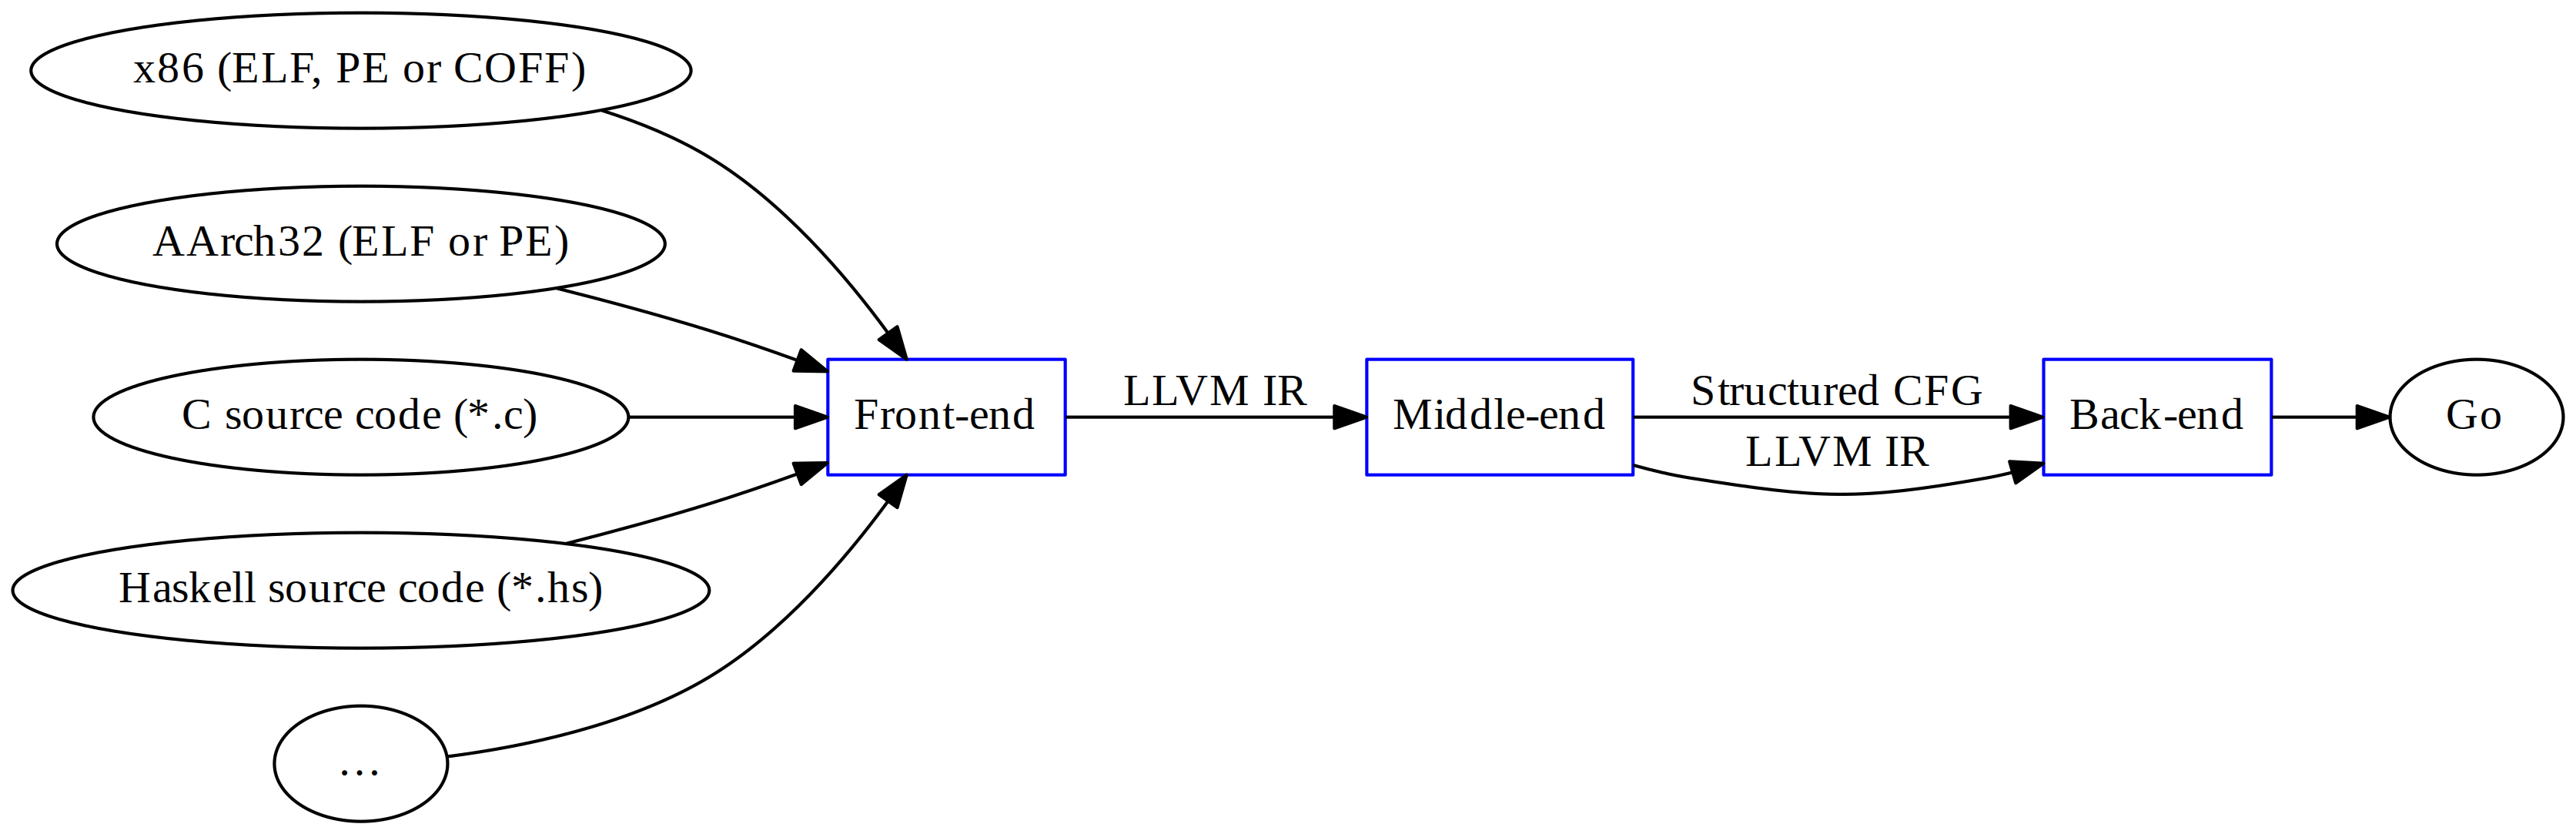
\includegraphics[width=\textwidth]{inc/6_design/decompilation_pipeline.png}
		\caption{The front-end of the decompilation pipeline translates a variety of inputs (e.g. native code or source code) to LLVM IR; the middle-end structures the LLVM IR through control flow analysis; and the back-end translates the structured LLVM IR to a high-level programming language (e.g. Go).}
		\label{fig:decompilation_pipeline}
	\end{center}
\end{figure}

The main benefit with this decompiler architecture is that it scales well when implementing support for additional source languages (e.g. MIPS or PowerPC assembly) and target languages (e.g. Python), as the general decompilation tasks only have to be implemented once. The decompiler architecture is an adaptation of the one presented by C. Cifuentes back in 1994 (as described in section \ref{sec:lit_review_decompilation_phases}), which was heavily inspired by the architecture of compilers that separated general optimisation tasks (e.g. constant propagation) from concerns related to the source programming language (e.g. C) and the target computer architecture (e.g. x86). The compiler architecture has been proven so effective at separating concerns that it remains in use today by several production-quality compilers \cite{llvm_architecture,gcc_architecture}.

% --- [ Front-end Components ] -------------------------------------------------

\subsection{Front-end Components}
\label{sec:front-end_components}

% TODO: Rewrite and clarify.

The front-end module is responsible for converting the input into LLVM IR. Two common scenarios exists, converting binary files (e.g. executables, shared libraries and relocatable object code) and converting source code (e.g. C, Haskell, Rust, …) into LLVM IR. The first scenario is presented in section \ref{sec:design_native_code_to_llvm_ir} and the second in section \ref{sec:compilers}.

% --- [ Subsubsections ] -------------------------------------------------------

% ~~~ [ Native Code to LLVM IR ] ~~~~~~~~~~~~~~~~~~~~~~~~~~~~~~~~~~~~~~~~~~~~~~~

\subsubsection{Native Code to LLVM IR}
\label{sec:design_native_code_to_llvm_ir}

There exist several open source projects which translate native code (e.g. x86 assembly of shared libraries in the PE file format) into LLVM IR. Three such projects have been reviewed in section \ref{sec:rel_work_native_code_to_llvm_ir}, which support different input file formats and machine architectures. These projects may be used as-is by the front-end module to translate low-level source languages into LLVM IR, as illustrated in figure \ref{fig:front-end_binary}.

\begin{figure}[htbp]
	\begin{center}
		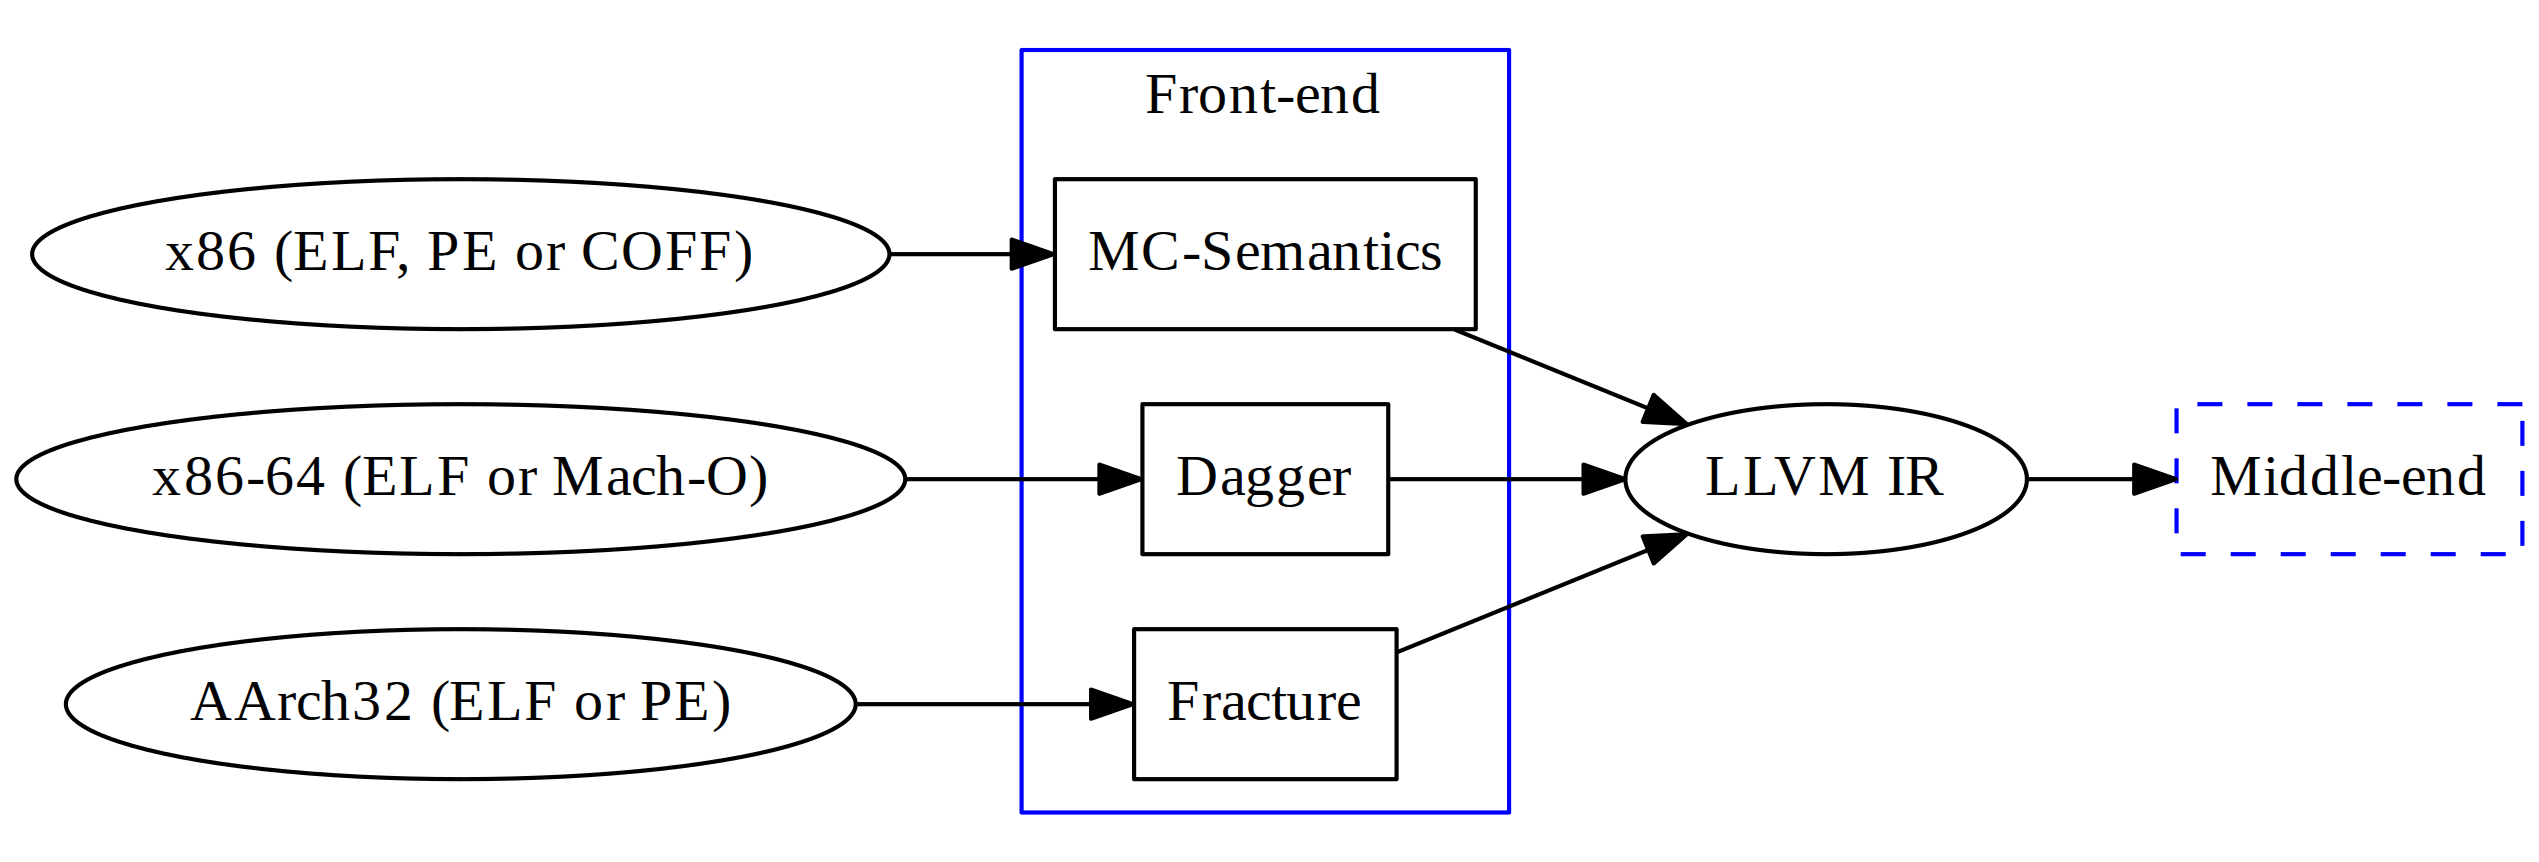
\includegraphics[width=\textwidth]{inc/6_design/front-end_binary.png}
		\caption{The three open source projects MC-Semantics, Dagger and Fracture translate native code of various architectures (e.g. x86, x86-64 and ARM) and file formats (e.g. ELF, PE, COFF and Mach-o) to LLVM IR.}
		\label{fig:front-end_binary}
	\end{center}
\end{figure}

% ~~~ [ Compilers ] ~~~~~~~~~~~~~~~~~~~~~~~~~~~~~~~~~~~~~~~~~~~~~~~~~~~~~~~~~~~~

\subsubsection{Compilers}
\label{sec:design_compilers}

One important aspect of utilizing the IR of a compiler framework, is that the decompilation pipeline automatically gains support for transpilation (i.e. translating one programming language into another) in addition to reverse compilation. An increasing number of open source compilers (e.g. Clang, GHC, \texttt{rustc}) are capable of translating a range of source languages (e.g. C, Haskell, Rust) into LLVM IR. These compilers may be used as-is by the front-end module (see figure \ref{fig:front-end_source}), thereby extending the supported source languages of the decompilation pipeline. Using this approach, the decompilation pipeline may translate $ n $ source languages into $ m $ target languages by implementing $ n + m $ front-end and back-end modules, instead of $ n \cdot m $ transpilers.

\begin{figure}[htbp]
	\begin{center}
		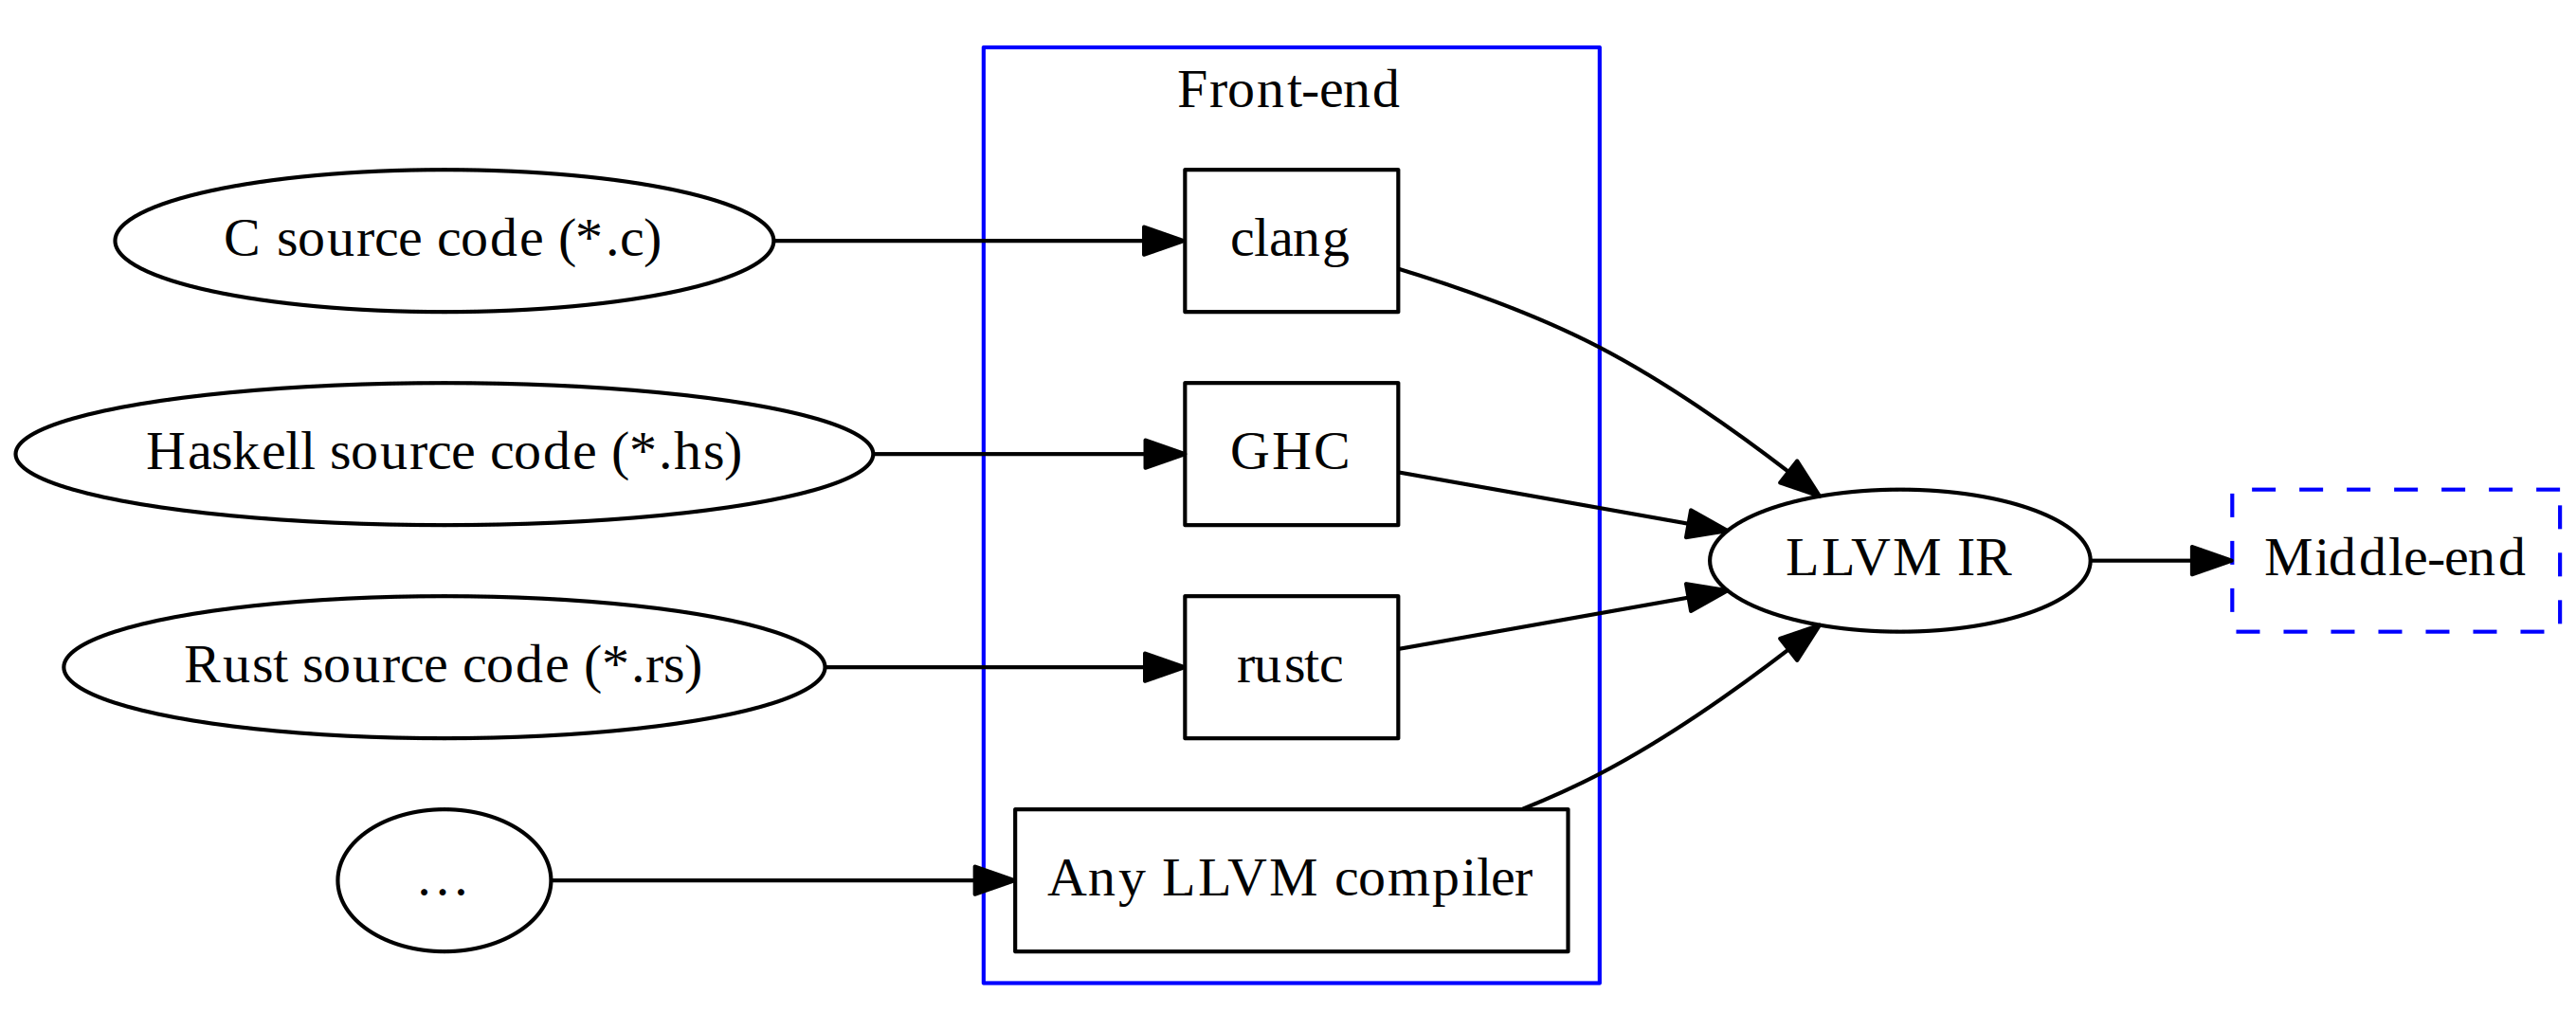
\includegraphics[width=\textwidth]{inc/6_design/front-end_source.png}
		\caption{Several open source compilers translate high-level programming languages into LLVM IR. Three such compilers are Clang, the Glasgow Haskell Compiler and the Rust compiler which translate C, Haskell and Rust respectively into LLVM IR.}
		\label{fig:front-end_source}
	\end{center}
\end{figure}

Another important aspect of utilizing LLVM IR, is that a wide range of optimizations have been implemented already by the LLVM compiler framework. This allows the front-end components to focus on translating the source languages into LLVM IR, without having to worry about producing highly optimised output. The LLVM IR may later be optimised by invoking the \texttt{opt} tool of LLVM to remove dead code, propagate constants, and promote memory accesses to registers, for instance.


% --- [ Middle-end Components ] ------------------------------------------------

% <howto>
% * more detailed design of individual components (design)

% <howto>
% * The intention is that the design should be detailed enough to provide a good guide for actual coding, including details of any particular algorithms to be used.

\subsection{Middle-end Components}

% TODO: Visualize the dependency graph of the "restructure" tool and describe in detail what input it expects and what output it produces.

% TODO: Write about. Input and output LLVM IR to operate well with components written in other languages. Output LLVM IR with information about high-level control structures stored in the basic block names or in metadata.

% TODO: Mention package division.

% TODO: Rewrite and clarify.

The middle-end is responsible for lifting the LLVM IR to a high-level representation through a series of decompilation passes. The \texttt{ll2dot} tool generates a CFG (in the DOT file format) for each function of a given LLVM IR input file. The \texttt{restructure} tool searches for subgraph isomorphisms of control flow primitives in a given CFG. Once located the nodes identified subgraph are merged into a single node which is labeled with the high-level control flow primitive. Successive iterations continue to simplify the CFG until only one node is left, at which point the high-level control flow primitive has been recovered. Should the \texttt{restructure} tool fail to reduce the graph into a single node, the graph is considered irreducible with regards to the supported high-level control flow primitives. The interaction between the front-end, the \texttt{ll2dot} and \texttt{restructure} tools of the middle-end and the back-end is illustrated in figure \ref{fig:middle-end}.

% TODO: Write about the choice of subgraph isomorphism search algorithm. The
% properties of the control flow graph allows us to optimize.
%
% \cite{subgraph_isomorphism_algorithms}

\begin{figure}[htbp]
	\begin{center}
		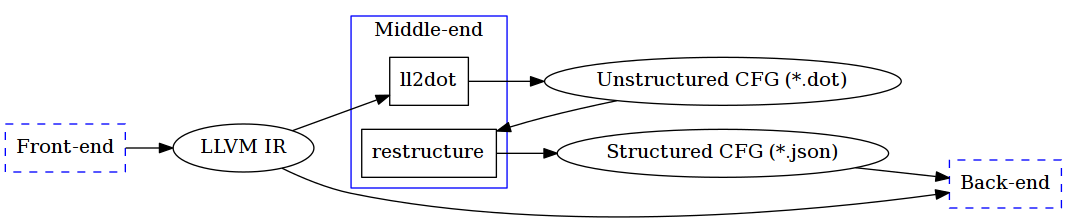
\includegraphics[width=\textwidth]{inc/middle-end.png}
		\caption{foo}
		\label{fig:middle-end}
	\end{center}
\end{figure}

% ~~~ [ Control Flow Graph Generation ] ~~~~~~~~~~~~~~~~~~~~~~~~~~~~~~~~~~~~~~~~

\subsubsection{Control Flow Graph Generation}
\label{sec:design_control_flow_graph_generation}

The control flow graph generation component generates a CFG for each function of a given LLVM IR assembly file. As described in section \ref{sec:lit_review_llvm_ir}, a function definition in LLVM IR consists of a set of basic blocks; and a basic block consists of zero or more non-branching instructions followed by a terminating instruction (such as \texttt{br} or \texttt{ret}) which changes the control flow. Therefore, the control flow graph generation component may focus on analysing the last instruction of each basic block, as they will determine the control flow.

To generate the CFG of a given function, a directed graph is created and populated with one node per basic block, and with zero or more directed edges between the nodes of the graph. The node names are determined by the basic block labels, and the directed edges are determined by the terminating instructions, as illustrated in figure \ref{fig:cfg_gen_example}.

\begin{figure}[htbp]
	\centering
	\begin{subfigure}[ht]{0.54\textwidth}
		\lstinputlisting[language=llvm, style=nasm, tabsize=2]{inc/cfg_gen_example.ll}
	\end{subfigure}
	\enskip
	\begin{subfigure}[ht]{0.22\textwidth}
		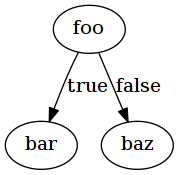
\includegraphics[width=\textwidth]{inc/cfg_gen_example.png}
	\end{subfigure}
	\caption{The return instructions of basic block \texttt{bar} and \texttt{baz} produces no directed edges, while the conditional branch instruction of basic block \texttt{foo} produces two directed edges, one for each target branch (i.e. \texttt{bar} and \texttt{baz}).}
	\label{fig:cfg_gen_example}
\end{figure}


The \texttt{ll2dot} tool generates CFGs from LLVM IR in the DOT file format, which is a well-defined textual representation of graphs used by the Graphviz project. One benefit of expressing CFGs in this format, is that the existing Graphviz tools may be facilitated to produce image representations of the CFGs; as demonstrated in appendix \ref{app:control_flow_graph_generation_example}.

% ~~~ [ Control Flow Analysis ] ~~~~~~~~~~~~~~~~~~~~~~~~~~~~~~~~~~~~~~~~~~~~~~~~

\subsubsection{Control Flow Analysis}
\label{sec:design_control_flow_analysis}

The key idea behind the control flow analysis (see section \ref{sec:control_flow_analysis}), is that high-level control flow primitives may be represented using directed graphs. The problem of structuring low-level code may therefore be rephrased as the problem of identifying subgraphs (e.g. the graph representation of high-level control flow primitives) in graphs (e.g. the CFGs of low-level code) without considering node names, as illustrated in figure \ref{fig:representation_and_identification_of_primitive}. This problem is generally referred to as \textit{subgraph isomorphism search} and has been well studied \cite{subgraph_isomorphism_algorithms}. Rephrasing the problem in this manner aligns with the design principle of giving each component access to the least amount of information required to successfully accomplish its task. The control flow analysis component is only given access to control flow information (e.g. CFGs), and is oblivious of the underlying LLVM IR. This enables the component to be reused as-is when analyzing the control flow of other languages, such as REIL.

\begin{figure}[htbp]
	\centering
	\begin{subfigure}[ht]{0.10\textwidth}
		\lstinputlisting[language=go, style=go, breaklines=false, numbers=none]{poster/inc/if.c}
		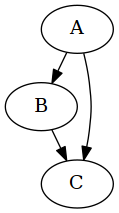
\includegraphics[width=\textwidth]{poster/inc/if.png}
	\end{subfigure}
	\enskip
	\begin{subfigure}[ht]{0.18\textwidth}
		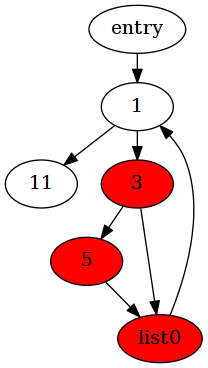
\includegraphics[width=\textwidth]{poster/inc/foo.png}
	\end{subfigure}
	\caption{The left side contains the pseudo-code (top left) and graph representation (bottom left) of an if-statement; if \texttt{A} is true then do \texttt{B} followed by \texttt{C}, otherwise do \texttt{C}. The right side highlights (in red) an identified isomorphism of the if-statement's graph representation, in the CFG of the \texttt{main} function presented in appendix \ref{app:clang_example}.}
	\label{fig:representation_and_identification_of_primitive}
\end{figure}

The \texttt{restructure} tool uses subgraph isomorphism search algorithms to locate isomorphisms of the graph representations of high-level control flow primitives in the CFG of a given function. The CFG is simplified by recursively replacing the identified subgraphs with single nodes until the entire CFG has been reduced into a single node; a step-by-step demonstration of which is presented in appendix \ref{app:control_flow_analysis_example}. By recoding the node names of the identified subgraph isomorphisms and the name of their corresponding high-level control flow primitives, a structured CFG may be produced in which all nodes are known to belong to a high-level control flow primitive; as demonstrated in appendix \ref{app:restructure_example}.

The pseudo-code and graph representations of the supported high-level control flow primitives are presented in figure \ref{fig:graph_representations} of section \ref{sec:control_flow_analysis}. Should the control flow analysis fail to reduce a CFG into a single node, the CFG is considered irreducible with regards to the supported high-level control flow primitives, in which case a structured CFG cannot be produced.

The \texttt{restructure} tool relies entirely on subgraph isomorphism search to produce structured CFGs (in JSON format) from unstructured CFGs (in the DOT file format). The supported high-level control flow primitives are defined using DOT files, thus promoting a data-driven design which separates data regarding the primitives from the implementation of the \texttt{restructure} tool. A major benefit with this approach is that the \texttt{restructure} tool may search for any high-level control flow primitive that can be expressed in the DOT file format, without any modification to the source code.

One limitation with this approach is that it does not support graph representations of high-level control flow primitives with a variable number of nodes, as they cannot be described in the DOT file format. For this reason, the \texttt{restructure} tool does not support the recovery of n-way conditionals (e.g. \texttt{switch}-statements). Furthermore, the current design enforces a single-entry/single-exit invariant on the graph representation of high-level control flow primitives. This prevents the recovery of infinite loops, as their graph representation has no exit node. A discussion of how these issues may be mitigated in the future is provided in section \ref{sec:design_validation}.


% --- [ Back-end Components ] --------------------------------------------------

\subsection{Back-end Components}
\label{sec:design_back-end_components}

The back-end module translates structured LLVM IR into a target high-level programming language, using two distinct stages. Firstly, the code generation stage translates LLVM IR into unpolished Go code by converting the individual instructions into equivalent Go statements and creating high-level control flow primitives for the various basic blocks, using the information of the structured CFGs (see section~\ref{sec:design_control_flow_analysis}). Secondly, the post-processing stage improves the quality of the unpolished Go code, through a series of source code transformations. The interaction between the middle-end, and the \texttt{ll2go} and \texttt{go-post} tools of the back-end is illustrated in figure~\ref{fig:back-end}.

\begin{figure}[htbp]
	\begin{center}
		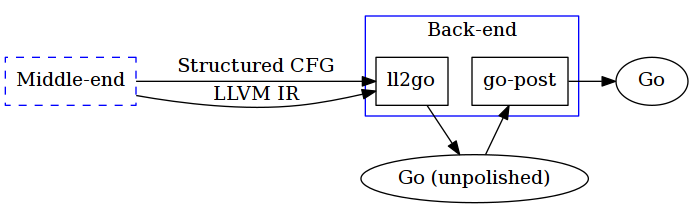
\includegraphics[width=0.8\textwidth]{inc/6_design/back-end.png}
		\caption{The back-end module decompiles structured LLVM IR into Go source code, using two components. The \texttt{ll2go} tool translates structured LLVM IR assembly into unpolished Go code, which is post-processed by the \texttt{go-post} tool to improve the quality of the output.}
		\label{fig:back-end}
	\end{center}
\end{figure}

The clear distinction between the two back-end stages aligns with the design principle of separation of concern. The code generation stage may focus on converting LLVM IR into equivalent Go code, without having to worry about the quality of the produced code. Similarly, the post-processing stage may focus on simplifying the Go code and make it more idiomatic, without any knowledge of the underlying LLVM IR. This enables the post-processing component to be reused as-is by other projects to improve the quality of Go code.

A tighter integration between the two stages could potentially produce a higher quality output, but there are no known issues preventing the decoupled stages from producing output of equivalent quality.

The decompilation pipeline aims to keep the back-end module as simple as possible, by delegating general decompilation tasks (e.g. control flow analysis, data flow analysis) to the middle-end module. This reduces the efforts required to implement additional back-ends, which add support for new target programming languages (e.g. Python).

% --- [ Subsubsections ] -------------------------------------------------------

% ~~~ [ Post-processing ] ~~~~~~~~~~~~~~~~~~~~~~~~~~~~~~~~~~~~~~~~~~~~~~~~~~~~~~

\subsubsection{Post-processing}
\label{sec:design_post-processing}

The post-processing stage post-processes the unpolished Go source code from the earlier stages of the decompilation pipeline, by applying a set of source code transformations. The \texttt{go-post} tool improves the quality of Go source code by declaring unresolved identifiers, applying Go conventions for exit status codes, propagating temporary variables into expressions, simplifying binary operations, removing dead assignment statements, and promoting the initialisation statement and post-statement of for-loops to the loop header; as demonstrated by the step-by-step refinement of the unpolished source code in presented appendix~\ref{app:post-processing_example}.



% === [ Implementation ] =======================================================

% <howto>
% * Write the implementation chapter plot heavy (as a novel)
%    - Problem/task
%    - What happened?
%    - How was is solved?
%
% * If the artifact isn't capable of doing everything that was wanted.
%     - Describe problems and reflect on how those problems where solved.
%
% * NOT screenshot (should go in appendix)
%
% * Process of development.
%
% * These are the descitions I made and why.
% * There are interesting problems and here is how I went about solving them.
% * Not just what, but why you did something. What my choices were and why I
%   choose the specific one.
%
% * In the course of the development some changes were made to the design.
% * In the process of doing the implementation, this was the initial design, and
%   these changes had to be made.
%
% Supervisor:
%    - What was this for, why did you do that?

% * Captivative reading
%    - Make the reading captivating; e.g. Dan Brown. And then X, and then Y.
%    - And then I had a problem, and what did I do about it; which lead to these Z.


\section{Implementation}
\label{sec:implementation}

% TODO: Add? Formal IR
% * No Formal Grammar for LLVM IR
% * Look for other people who has done work in this field
% 	- Reed Koter (MIPS), https://code.google.com/p/llvm-assembly-language-formal-specification/
% * Collaborate on the Formal Grammar.

% TODO: Note from Janka: The Implementation section should be strictly related to the software itself.

% TODO: Brainstorm about which sections are actually relevant and how they should be structured.

% TODO: Mention the following trivias:
%    - Identify unused tokens (hash and backspace) in the C++ code base and submit a patch which was commited to remove these. (http://reviews.llvm.org/D7248)
%    - Discuss API design with members of the open source community.
%    - Ask experienced LLVM developers of insight into possible inconsistencies with LLVM IR. Some highlighted inconsistent behaviour and some were intended behaviour. (LLVM-dev mailing list)

% Hints for Computer System Design (1983) - Butler Lampson
%    "Handle normal and worst case seperately"

foo

% === [ Subsections ] ==========================================================

% --- [ Language Considerations ] ----------------------------------------------

% <howto>
% * choice of programming language(s) (implementation)

\subsection{Language Considerations}

As stated by H. Mayer in 1989, \textit{``No programming language is perfect. There is not even a single best language; there are only languages well suited or perhaps poorly suited for particular purposes. Understanding the problem and associated programming requirements is necessary for choosing the language best suited for the solution.''} \cite{no_perfect_lang_quote} This project seeks to explore the potential of a compositional approach to decompilation, and the components of the decompilation pipeline will require support for analysing and manipulating source code, and interacting with LLVM IR. The Go programming language emphasises composition at its core and provides extensive support for source code analysis, as indicated by the vast number of tools developed for analysing and manipulating Go source code (examples of such tools are given in section \ref{sec:ver_continuous_integration}). As the LLVM compiler framework is written in C++, several projects (e.g. Dagger, Fracture, MC-Semantics) have chosen this language for interacting with LLVM IR. Meanwhile, a mature LLVM IR library is yet to be written for Go.

In 2012 Rob Pike (one of the Go language inventors) gave a talk titled \textit{``Less is exponentially more''} which included a personal description of the historic events leading up to the inception of Go. The starting point of the language was C, not C++, which Go aimed to simplify further by removing cruft. This is in direct contrast to the direction of C++ which gains more features with each passing release. The \textit{less is more} mindset is deeply rooted in the mentality of Go developers, and there is a strong emphasis on the use of composition to solve problems, as indicated by the following extract from Rob Pike's talk.

\begin{quote}
	\itshape
	``If C++ and Java are about type hierarchies and the taxonomy of types, Go is about composition.

	Doug McIlroy, the eventual inventor of Unix pipes, wrote in 1964 (!):

	\begin{quote}
		We should have some ways of coupling programs like garden hose--screw in another segment when it becomes necessary to massage data in another way. This is the way of IO also.
	\end{quote}

	That is the way of Go also. Go takes that idea and pushes it very far. It is a language of composition and coupling.''
	\normalfont
	- Rob Pike, 2012 \cite{less_is_more}
\end{quote}

Every aspect of Go development embodies the UNIX philosophy (see figure \ref{fig:unix_philosophy}), which is no surprise as Ken Thompson (one of the original inventors of UNIX) is part of the core Go team.

\begin{figure}[htbp]
	\begin{center}
		\begin{quote}
			\textit{``Write programs that do one thing and do it well. Write programs to work together.''} \cite{art_of_unix}
		\end{quote}
		\caption{The UNIX philosophy.}
		\label{fig:unix_philosophy}
	\end{center}
\end{figure}

To conclude the language considerations, Go has been chosen as the primary language for the decompilation pipeline based on its simplicity and emphasis on composition. Furthermore, the Go standard library includes production quality support for lexing and parsing of Go source code. The language may therefore be a good candidate for developing lexers and parsers for LLVM IR, as will be further discussed in section \ref{sec:impl_llvm_ir_library}.

% --- [ LLVM IR Library ] ------------------------------------------------------

\subsection{LLVM IR Library}
\label{sec:impl_llvm_ir_library}

Early on in the project it was believed that the control flow analysis stage would operate on CFGs that were tightly coupled with an in-memory representation of LLVM IR. This motivated the search for a LLVM IR library with a carefully considered API and set of data structures (objective \ref{itm:obj_ir_library}). While there existed a library which provides Go bindings for LLVM, the API of this library felt awkward to use and was too heavily influenced by the underlying C and C\texttt{++} libraries; as further described in section \ref{sec:impl_go_bindings_for_llvm}. The interaction with the LLVM IR library would critically influence the design and implementation of the decompilation components. For this reason it was decided that a set of pure Go libraries would be implemented for interacting with LLVM IR, even if it would require a considerable amount of work.

The LLVM IR libraries were intentially developed as reusable components for compilers, decompilers and other semantic analysis tools. To assess the requirements of LLVM-based compilers, a public discussion was held with the developers of the open source \texttt{llgo} compiler, who clarified its specific requirements\footnote{Requirements: \url{https://github.com/llir/llvm/issues/3}}. Fredrik Ehnbom, who is one of the \texttt{llgo} developers, has remained involved with the development of the LLVM IR libraries, by participating in API discussions, conducting code reviews, and submitting patches for performance improvements\footnote{Use binary search for keyword lexing: \url{https://github.com/llir/llvm/pull/11}} (these code changes have not yet been merged, as the project artefacts are required to be developed independently).

The first component to be implemented was the LLVM IR lexer, which tokenizes LLVM IR assembly. In addition to the LLVM IR language specification, the implementation of the reference lexer in LLVM was reviewed to establish a full listing of the valid tokens in LLVM IR. This review uncovered two tokens which were defined but never used in the code base of LLVM. In collaboration with members of the LLVM community, a patch was commited to the LLVM code base which removed these tokens\footnote{Remove unused tokens from AsmParser: \url{http://reviews.llvm.org/D7248}}.

The design of the LLVM IR lexer has been hugely influenced by a talk given by Rob Pike in 2011, titled \textit{``Lexical Scanning in Go''} \cite{lexical_scanning_in_go}. In this talk, Pike introduces the notion of a state function which is a function that returns a state function. The state of the lexer is represented by the active state function, which may transition into another stage by returning the corresponding state function. For instance, when \texttt{lexLineComment} is active, the context of the lexer is known to be a line comment. Any character is valid within line comments, except new lines which terminate the token; at which point an unknown token on the succeeding line is lexed by returning the \texttt{lexToken} state function.

The LLVM IR assembly language requires no separators (e.g. whitespace characters, semicolons) between tokens. This made it very difficult to determine where one token ends and another starts, as further indicated by inconsistent behaviour for separating tokens in the reference implementation of the LLVM lexer. The solution to this issue was inspired by the Go language specification\footnote{The Go Programming Language Specification: \url{https://golang.org/ref/spec}} which states that \textit{``the next token is the longest sequence of characters that form a valid token''}, thus defining a consistent behaviour.

A formal grammar of the LLVM IR language would have facilitate the implementation of the LLVM IR libraries. As no such grammar had been officially endorsed, other sources were cross-referenced to learn about the low-level details of the language, such as its token set and details regarding the type system. This work uncovered a number of potential inconsistencies between the language reference, the implementation, and official blog posts. After discussing these issues with more experienced LLVM developers on the LLVM-dev mailing list, it could be concluded that some issues highlighted inconsistent behaviours while others were working as intended.

The cheer size of LLVM IR was at times discouraging and the project time constrains forced the implementation of subsets within every aspect of the language. LLVM IR may have started out as a simple, minimalistic and platform-independent low-level IR, but this is no longer the case. As time went by and as the project rose in popularity, more and more developers joined the project. In 2014 more than five hundred commits were submitted to the LLVM code base each month. Keeping these changes consistent and the overall system simple is a massive challenge.

It was at times very tempting to switch to REIL instead of LLVM IR, as REIL is a minimal, consistent and clean language. The adaptation of REIL in the open source community was however limited, and there had been no public news announcements since Google acquired the company back in 2011. Furthermore, the REIL language lacks the notion of basic blocks which would complicate the control flow analysis.

After months of development it had become clear that the task of implementing libraries for LLVM IR was way more time consuming than initially anticipated. The project time constrains forced the re-evaluation of using the Go bindings for LLVM, which gave rise to a seemingly small but hugely influential idea. The control flow analysis stage should operate entirely on graph data structures, thus making it unaware of LLVM IR. This idea effectively mitigated the risk of being influenced by the API of the Go bindings for LLVM, and gave rise to the data-driven design of the control flow analysis component, as further described in section \ref{sec:design_control_flow_analysis}. From this point on, the focus shifted to implementing working artefacts which utilised the Go bindings for LLVM IR, as further described in section \ref{sec:impl_go_bindings_for_llvm}.

% --- [ Control Flow Graph Generation Tool ] -----------------------------------

\subsection{Control Flow Graph Generation Tool}

foo

% --- [ Subgraph Isomorphism Search Algorithm ] --------------------------------

\subsection{Subgraph Isomorphism Search Algorithm}

Implementing the subgraph isomorphism search algorithm was without doubt the most difficult endeavour of the entire project. It took roughly five iterations of implementing, evaluating and rethinking the algorithm to find an approach which felt right and another two iterations to develop a working implementation which passed all the test cases.

foo

% TODO: Incorporate notes from iso_algorithm_notes.txt.

% --- [ Control Flow Analysis Tool ] -------------------------------------------

\subsection{Control Flow Analysis Tool}

foo

% --- [ Code Generation Tool ] -------------------------------------------------

\subsection{Code Generation Tool}

foo

% --- [ Post-processing Tool ] -------------------------------------------------

\subsection{Post-processing Tool}

foo

% --- [ Documentation ] --------------------------------------------------------

\subsection{Documentation}

A set of source code analysis tools are used to automate the generation and presentation of documentation. The main benefit of this approach is that only one version of the documentation has to be maintained and it is kept within the source code, thus preventing it from falling out of sync with the implementation. UNIX manual pages are generated for command line tools using \texttt{mango}\footnote{Generate Man pages from Go source: \url{https://github.com/slyrz/mango}}, which locates the relevant comments and command line flag definitions in the source code. Library documentation is presented using \texttt{godoc}\footnote{Godoc extracts and generates documentation for Go programs: \url{https://golang.org/cmd/godoc}} (a tool similar to \texttt{doxygen}), and may be accessed through a web or command line interface.

The GoDoc.org server hosts an instance of \texttt{godoc} which presents the documentation of publicly available source code repositories. An online version of the documentation has been made available for each artefact using this service.

\begin{itemize}
	\item Library for interacting with LLVM IR (\textit{work in progress}) \\ \url{https://godoc.org/github.com/llir/llvm}
	\item Control flow graph generation tool \\ \url{https://godoc.org/decomp.org/x/cmd/ll2dot}
	\item Subgraph isomorphism search algorithms and related tools \\ \url{https://godoc.org/decomp.org/x/graphs}
	\item Control flow analysis tool \\ \url{https://godoc.org/decomp.org/x/cmd/restructure}
	\item Go code generation tool (\textit{proof of concept}) \\ \url{https://godoc.org/decomp.org/x/cmd/ll2go}
	\item Go post-processing tool \\ \url{https://godoc.org/decomp.org/x/cmd/go-post}
\end{itemize}


% === [ Verification ] =========================================================

\section{Verification}

% TODO: Add meta-text which mentions verification, performance testing and
% Continuous Integration.

foo

% --- [ Correctness of Implementation ] ----------------------------------------

\subsection{Correctness of Implementation}

foo

\subsubsection{Test Cases}

% TODO: Add
%    - Use the Clang compiler to produce test cases, as it is capable of emitting LLVM IR from C source code. The goal will be to reconstruct the high- level control flow structures (such as for- loops, if-else statements, etc) of the original C code from the LLVM IR.

foo

\begin{figure}[htbp]
	\begin{center}
		\begin{verbatim}
$ go test -v github.com/mewrev/graphs/iso
=== RUN TestCandidates
--- PASS: TestCandidates (0.02s)
=== RUN TestEquationSolveUnique
--- PASS: TestEquationSolveUnique (0.00s)
=== RUN TestEquationIsValid
--- PASS: TestEquationIsValid (0.22s)
=== RUN TestIsomorphism
--- PASS: TestIsomorphism (0.18s)
=== RUN TestSearch
--- PASS: TestSearch (0.20s)
PASS
ok     github.com/mewrev/graphs/iso   0.62s
		\end{verbatim}
		\caption{An extract of the test cases used to verify the subgraph isomorphism search algorithm, as visualized by \texttt{go test}.}
		\label{fig:iso_test_cases}
	\end{center}
\end{figure}

\subsubsection{Code Coverage}

The code coverage is a measurement of how much of the code is exercised by the test cases.

% TODO: Add note on how the Go code coverage is calculated.

While developing a lexer for the LLVM IR assembly language the intention was to strive for a 100\% code coverage of any code related to lexing and not related to input output errors (e.g. ``file not found'' errors). As illustrated in \cref{fig:lexer_code_coverage}. The rigid testing made it possible to locate and correct a number of faulty assumptions in the lexing logic.

\begin{figure}[htbp]
	\begin{center}
		\begin{verbatim}
$ go test -coverprofile=lexer.out github.com/mewlang/llvm/asm/lexer
$ go tool cover -func=lexer.out
llvm/asm/lexer/lexer.go:36:    ParseFile      80.0%
llvm/asm/lexer/lexer.go:118:   emit           100.0%
llvm/asm/lexer/lexer.go:139:   next           100.0%
llvm/asm/lexer/lexer.go:158:   accept         100.0%
llvm/asm/lexer/state.go:38:    lexToken       100.0%
llvm/asm/lexer/state.go:131:   lexComment     100.0%
…
llvm/asm/lexer/state.go:364:   lexQuote       100.0%
llvm/asm/lexer/state.go:585:   unescape       100.0%
total:                         (statements)   97.5%
		\end{verbatim}
		\caption{A summary of the code coverage for a selection of the LLVM IR lexer functions, as visualized by the \texttt{cover} tool.}
		\label{fig:lexer_code_coverage}
	\end{center}
\end{figure}

The use of code coverage heat maps, which track how often statements are exercised by the test cases, were invaluable when stress testing the subgraph isomorphism search algorithm, and they were able to identify several tricky corner cases. foo \cref{fig:iso_heat_map}

\begin{figure}[htbp]
	\begin{center}
		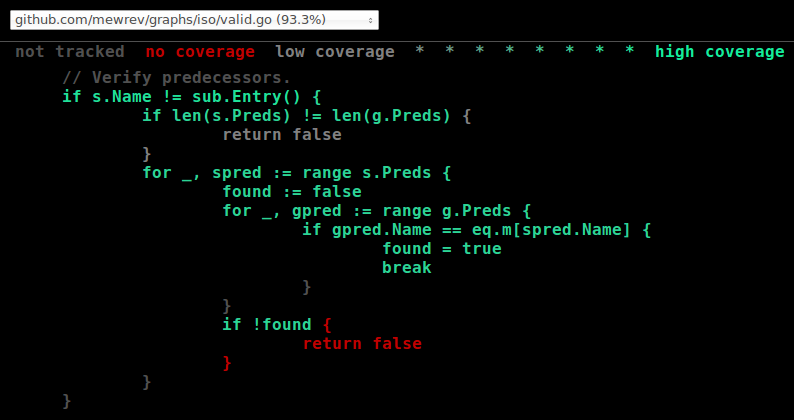
\includegraphics[width=\textwidth]{inc/iso_code_coverage_heat_map.png}
		% TODO: Fix caption text.
		\caption{Extract from the code coverage of the subgraph isomorphism search algorithm, represented as a heat map where red indicates that a statement was never visited and the intensity of green indicates the number of times a statement was visited. where bright green represents a statements that has been visited several times, faint green a statement only visited a few times, and red a statement that has never been visited.}
		\label{fig:iso_heat_map}
	\end{center}
\end{figure}

foo

% --- [ Performance ] ----------------------------------------------------------

\subsection{Performance}

% TODO: Rewrite, cleanup and verify (especially the \theta(...) claims!).

Profiling was put to good use when optimizing the lexer, the code base of which is rather straight forward. When estimating the runtime complexity of the subgraph isomorphism search algorithm however the use of intuition and algorithm research was far more valuable. For this specific task the generic problem (subgraph isomorphism search of arbitrary input graphs) could be simplified (TODO: use generalized instead of simplified?) to a much easier problem as every node of the graph were known to be connected (TODO: find the succinct term in graph theory to express this concept). Exploiting this property lead to an algorithm that had a runtime complexity of $ \Theta(n*m) $ where $ m $ is known to be small rather than $ \Theta(n^m) $ as is the case for a brute force algorithm and $ \Theta(n^log(m)) $ (TODO: Find the correct runtime complexity of the Hillman iso search algo) as was the case of the Hillman subgraph isomorphism search algorithm which is capable of solving the generic case, improving on the brute force approach by applying heuristics (TODO: is heuristics the right word to use here?) to prune the search space.

In summary, using profiling is great for simple problems. Using algorithm research, runtime complexity theory and intuition is needed for complex problems. Knowledge about specific properties of the problem which may be exploited.

foo

\subsubsection{Benchmarks}

percentage delta.

\texttt{benchcmp}

foo

\subsubsection{Profiling}

% TODO: Add bottle neck example
%    inc/lexer_pprof_before.svg

% TODO:
%    - CPU profiling
%       go test -cpuprofile=a.out
%    - Memory profiling
%       go test -memprofile=a.out

\texttt{go tool pprof}

foo

% --- [ Continuous Integration ] -----------------------------------------------

\subsection{Continuous Integration}

The Continuous Integration (CI) practise originated from the Extreme Programming methodology \cite{xp} but has reached a much broader audience in recent years. Today most large scale software projects rely on CI server farms which continuously compile and test new versions of the source code.

This project makes use of Travis CI, which is tightly integrated with GitHub, to run a series of automated tests for each commit to the source code repository. The tests are varied and range from identifying source code formatting and coding style issues to monitoring the build status and test coverage. A future ambition is to run benchmarks for each commit to quickly identify performance regressions.

\subsubsection{Source Code Formatting}

Instead of relying on a formatting style guide the Go project enforces a single formatting style using \texttt{gofmt} (a tool similar to \texttt{indent}) which automatically formats Go source code. The adoption of this tool is widespread within the Go community as indicated by a survey conducted back in 2013. The survey found that 70\% of the publicly available Go packages were formatted according to the rules of \texttt{gofmt} \cite{gofmt_70percent}, a figure which is likely to have increased since then.

Using a single formatting style for all Go source code may at first seem like a small deal, but the advantages are vast. It becomes easier to write code as one may focus on the problem at hand rather than minor formatting issues. Similarly it becomes easier to read code when it is formatted in a familiar and uniform manner. We may focus our entire attention at understanding the semantics of the code without being distracted by inconsistent or unfamiliar formatting. And perhaps most importantly, it prevents useless discussions about which formatting style is the right one.

Several text editors supports adding pre-save hooks which executes a command to pre-process the text before saving it. This mechanism may be used with the \texttt{gofmt} tool to automatically enforce its formatting style each time a source file is saved. One of the CI tests catches and reports incorrectly formatted source code, should a programmer forget to install such a hook.

\subsubsection{Coding Style}

% There exists linting software for several programming languages which detect and report issues related to coding style.

% The established conventions

% There exists several official sources which describe the coding conventions

% Effective in the sense that

% Learning the syntax of a programming langauge and its key features is not enough to ensure

% TODO: Add paragraph refering to Effective Go.
% \cite{effective_go}

% TODO: cyclocomplexity...?

% To write idiomatic code in any programming language requires at least a resonable understanding of underlying design decisions which drove the development of the language.

% a understanding of its is required of the

% Learning to program effectively in a new language requires much more than simply learning the syntax of the language and its key features. A reasonable understanding of the underlying design decisions behind the language,

% When learning a new programming language it is important to understand its ideoms and the established conventions.

% The conventions

% Coding conventions


\texttt{golint}

% * Key word, conventions.
%
% := type inference.
% naming conventions
% documentation comments
% error messages

\cite{golint}

foo

\subsubsection{Code Correctness}

\texttt{go vet}

foo

\subsubsection{Build Status}

\texttt{go get}

foo

\subsubsection{Test Cases}

\texttt{go test}

foo

\subsubsection{Code Coverage}

\texttt{go test -cover}

foo

\subsubsection{Data Race Detection}

\texttt{go test -race}

foo

% === [ Evaluation ] ===========================================================

\section{Evaluation}

foo

% --- [ Evaluation against Requirements ] --------------------------------------

\subsection{Evaluation against Requirements}

foo

% --- [ TODO ] -----------------------------------------------------------------

\subsection{TODO}

foo

% --- [ Profiling and Benchmarks ] ---------------------------------------------

\subsection{Profiling and Benchmarks}

foo

% === [ Conclusion ] ===========================================================

% <howto>
% * Reflections on what you have personally learned from this and lessons for the future.
% * Reflect on how problems were solved in the conclusions chapter.
% * How well you implemented methodologies.
% * How successful the development was.
% * Reflective writing on what you've done.

% <howto> Relationship between sections.
%
%    Introduction ---> Conclusions
%                         ^
%                         |
%    Literature Review ---+

\section{Conclusion}
\label{sec:conclusion}

This section concludes the project report with subjective reflections from the author. For the remainder of this section I will switch to a first person narrative.

% === [ Subsections ] ==========================================================

% --- [ Project Summary ] ------------------------------------------------------

\subsection{Project Summary}

% TODO: Re-read one last time.

Reverse engineering has fascinated me for quite some time and I have experimented with a variety of tools, ranging from disassemblers and decompilers to debuggers and tracers. Many tools have been outstanding on an individual level and some have featured powerful extensibility through plugin and scripting support. I have never been bothered by the capabilities of these tools, but rather by the workflow they enforce and the environment they lock you in.

The de facto tools for binary analysis are monolithic in nature with regards to the end-user, as they do not expose their individual components. Imagine trying to reuse the control flow analysis of IDA Pro and the Hex-Rays Decompiler to implement control flow aware folding support in an IDE for x86 assembly development (e.g. group and toggle assembly code segments based on their corresponding high-level control flow structures). This idea is not limited by any technical issues; IDA Pro and the Hex-Rays Decompiler have support for recovering high-level control flow primitives from x86 assembly. If the IDE was given access to the control flow analysis component it would be trivial to implement sophisticated folding support for x86 assembly.

Having worked extensively within a UNIX environment, I have grown accustomed to a workflow that allows you to \textit{combine} individual tools in amazing ways; pipe the input from one tool into another which transforms, massages or interprets the data in a specific way. This background instilled me with a belief that the decompilation workflow could be facilitated by implementing a decompilation pipeline composed of individual and reusable components. Throughout the course of this project several independent components have been implementing, including a control flow graph generation tool which translates LLVM IR assembly into a control flow graph (represented in the DOT file format), a control flow analysis tool which identifies high-level control flow primitives in control flow graphs, a code generation tool which translates LLVM IR assembly into unpolished Go source code, and a post-processing tool which polishes the Go source code to make it more idiomatic.

These components have been combined with open source tools from other projects to form the foundation of a decompilation pipeline, which has been proven capable at recovering nested pre-test and post-test loops (e.g. \texttt{for} and \texttt{do-while} loops), and 1-way and 2-way (e.g. \texttt{if} and \texttt{if-else} statements) conditionals from LLVM IR assembly. The middle-end module of the decompilation pipeline uses an intermediate representation (LLVM IR) to separate heavy decompilation tasks (e.g. control flow analysis) from concerns related to the source (e.g. x86 assembly) and target (e.g. Go) language; thus making it easy to implement additional front-ends (e.g. support for MIPS assembly) or back-ends (e.g. support for Python output).

% --- [ Future Work ] ----------------------------------------------------------

\subsection{Future Work}
\label{sec:future_work}

The primary focus for planned future work is to stress test the design of the decompilation pipeline and its individual components. A secondary focus is to improve the quality and the reliability of the components. A tertiary focus is to extend the capabilities of the decompilation pipeline. This prioritization strives to validate the core of the system before extending it.

% ~~~ [ Design Validation ] ~~~~~~~~~~~~~~~~~~~~~~~~~~~~~~~~~~~~~~~~~~~~~~~~~~~~

\subsubsection{Design Validation}
\label{sec:design_validation}

The principle of separation of concern has influenced every aspect of the design of the decompilation pipeline and its individual components. Conceptually, the components of the decompilation pipeline are grouped into three modules which separate concerns regarding the source language (front-end module), the general decompilation tasks (middle-end module), and the target language (back-end module). This conceptual separation is a vital aspect of the decompilation pipeline design, and it will therefore be thoroughly examined. Should a component violate the principle of separation of concern, either in isolation or within the system as a whole, it must be redesigned or reimplemented. To identify such issues, key areas of the decompilation pipeline will be extended to put pressure on the design.

Firstly, an additional back-end (e.g. support for Python as a target language) will be implemented to put pressure on the design of the middle-end module. The second back-end would only be able to leverage the target-independent information of the general decompilation tasks (e.g. control flow analysis) if the middle-end module was implemented correctly.

Secondly, a key component (e.g. data flow analysis) will be implemented in a separate programming language (e.g. Haskell, Rust, Prolog, …) to validate the language-agnostic aspects of the design. This component would only be able to interact with the rest of the decompilation pipeline, through well-defined input and output (e.g. LLVM IR, JSON, DOT, …), if the other components were implemented correctly.

The separation of the front-end and middle-end has already been validated. These modules are only interacting through an intermediate representation (i.e. LLVM IR), and a variety of source languages are already supported by the front-end module which consists of components from several independent open source project (e.g. Dagger, Fracture, MC-Semantic, Clang, …).

The design of the control flow analysis component has both advantages and limitations, as discussed in section \ref{sec:design_control_flow_analysis}. The most significant limitation is the lack of support for control flow primitives with a variable number of nodes in their graph representation (e.g. n-way conditionals). To gain a better understanding of this issue, an analysis of control flow primitives from different high-level languages will be conducted. Should the n-node control flow primitives prove to be rare, hard-coded support for n-way conditionals (e.g. \texttt{switch}-statements) and similar control flow primitives would suffice. Otherwise, a general solution to the problem will be required (such as the introduction of a domain specific language which describes dynamic properties of the nodes and edges in DOT files). The OpenCL decompiler presented by Moll solved this problem by converting n-way conditionals into a set of 2-way conditionals \cite{decomp_of_llvm}.

% ~~~ [ Reliability Improvements ] ~~~~~~~~~~~~~~~~~~~~~~~~~~~~~~~~~~~~~~~~~~~~~

\subsubsection{Reliability Improvements}

As described in section \ref{sec:go_bindings_for_llvm}, there are many reliability issues caused by the Go bindings for LLVM. To mitigate these issues a pure Go library is being developed for interacting with LLVM IR (see section \ref{sec:llvm_ir_library}). This library will be reusable by other projects, and the requirements of the third-party Go compiler \texttt{llgo}\footnote{LLVM-based compiler for Go: \url{https://llvm.org/svn/llvm-project/llgo/trunk/README.TXT}} are actively being tracked\footnote{Requirements · Issue \#3: \url{https://github.com/llir/llvm/issues/3}}.

To ensure reliable interoperability between components written in different programming languages, the intermediate representation (i.e. LLVM IR) of the decompilation pipeline must be well-defined. Previous efforts to produce a formal grammar for LLVM IR have only focused on subsets of the language (as mentioned in section \ref{sec:req_llvm_ir_library}), and no such grammar has been officially endorsed. Producing an official formal specification for LLVM IR would require huge efforts, but it would enable interesting opportunities. For instance, with a formal grammar it would be possible to create a tool which automatically generates gramatically correct LLVM IR assembly which may be used to verify the various implementation of LLVM IR. This approach has been used by the GoSmith tool to generate random, but legal, Go programs which have uncovered 31 bugs in the official Go compiler, 18 bugs in the Gccgo compiler, 5 bugs in the \texttt{llgo} compiler, and 3 bugs in the language specification \cite{gosmith}.

% ~~~ [ Extended Capabilities ] ~~~~~~~~~~~~~~~~~~~~~~~~~~~~~~~~~~~~~~~~~~~~~~~~

\subsubsection{Extended Capabilities}

% Several extensions to the decompilation pipeline are planned, apart from the second back-end and the data flow analysis component already described in section \ref{sec:design_validation}.

% In programs written in C

% The post-processing stage of the Go back-end can easily be extended to make the output more idiomatic.

% The output of the Go back-end will be made mode idiomatic by introducing further post-processing stages.

% Further post-processing stages will be added to the Go back-end to make the output more idiomatic.

% TODO: Add grind (add footnote to rsc's grind tool)

In the far future, a type analysis component will be implement to support type recovery during decompilation. As type analysis requires type constraints equations to be solved, the component will be implemented in a language with good support support for constraints programming (e.g. Prolog). At this stage, more research is required to determine how generic type inference algorithms (e.g. Algorithm W \cite{algorithm_w}) may influence the design.

% --- [ Personal Development ] -------------------------------------------------

\subsection{Personal Development}

This is the largest project I have undertaken in my life and I feel satisfied with the outcome and proud of what I have been able to accomplished. It has re-enforced my belief that any problem is solvable when broken into smaller subproblems and instilled me with a feeling that anything is possible. The project has allowed me to mature as a software engineer and I now feel more confident in utilizing best practices such as TDD, CI and semantic versioning. I have also matured as a developer and gained experience with implementing a semi-large project and structuring it into several smaller self-contained projects.

If I were to redo the project today, I wish someone would have told me about the critical importance of effective time management, and then told me again to let it sink in. In the beginning of the project I used coarse time management and assigned bi-weekly deadlines to larger tasks. While some tasks were completed ahead of schedule, many were postponed. Later on it became apparent that accurate time estimates could only be given when larger tasks were broken down into sufficiently small sub-tasks. Towards the end of the project I used more granular time management and split larger tasks into sub-tasks that could be completed in a couple of days. For software development tasks the former technique (coarse time management) worked well and for report writing tasks the latter technique (granular time management) was most effective.

% TODO: Recommendations: If I were to redo the project today, I wish someone would have told me that xxx.

% --- [ Final Thoughts ] -------------------------------------------------------

\subsection{Final Thoughts}

My happiest moment during the project was when the larger components started working and could be connected to form a complete system. It feels great having started out with a vague idea of how the decompiler could work, gradually gaining new insights and refining its design after researching and building on the knowledge of others, developing and iteratively reimplementing the various components until they felt just right, finally arriving at a working prototype and seeing the full system in action! If there is one key idea I want to leave you with it is that the composition of independent components, each with a single purpose and well-defined input and output, is a powerful concept for solving complex problems.



% === [ References ] ===========================================================

\printbibliography[heading=bibintoc]

% === [ Appendices ] ===========================================================

% TODO: Remember to include the appendices.
%% === [ Appendices ] ===========================================================

\appendix
\setcounter{secnumdepth}{0}
\section{Appendices}
\setcounter{secnumdepth}{3}
\renewcommand{\thesubsection}{\Alph{subsection}}

% --- [ Project Initiation Document ] ------------------------------------------

\subsection{Project Initiation Document}

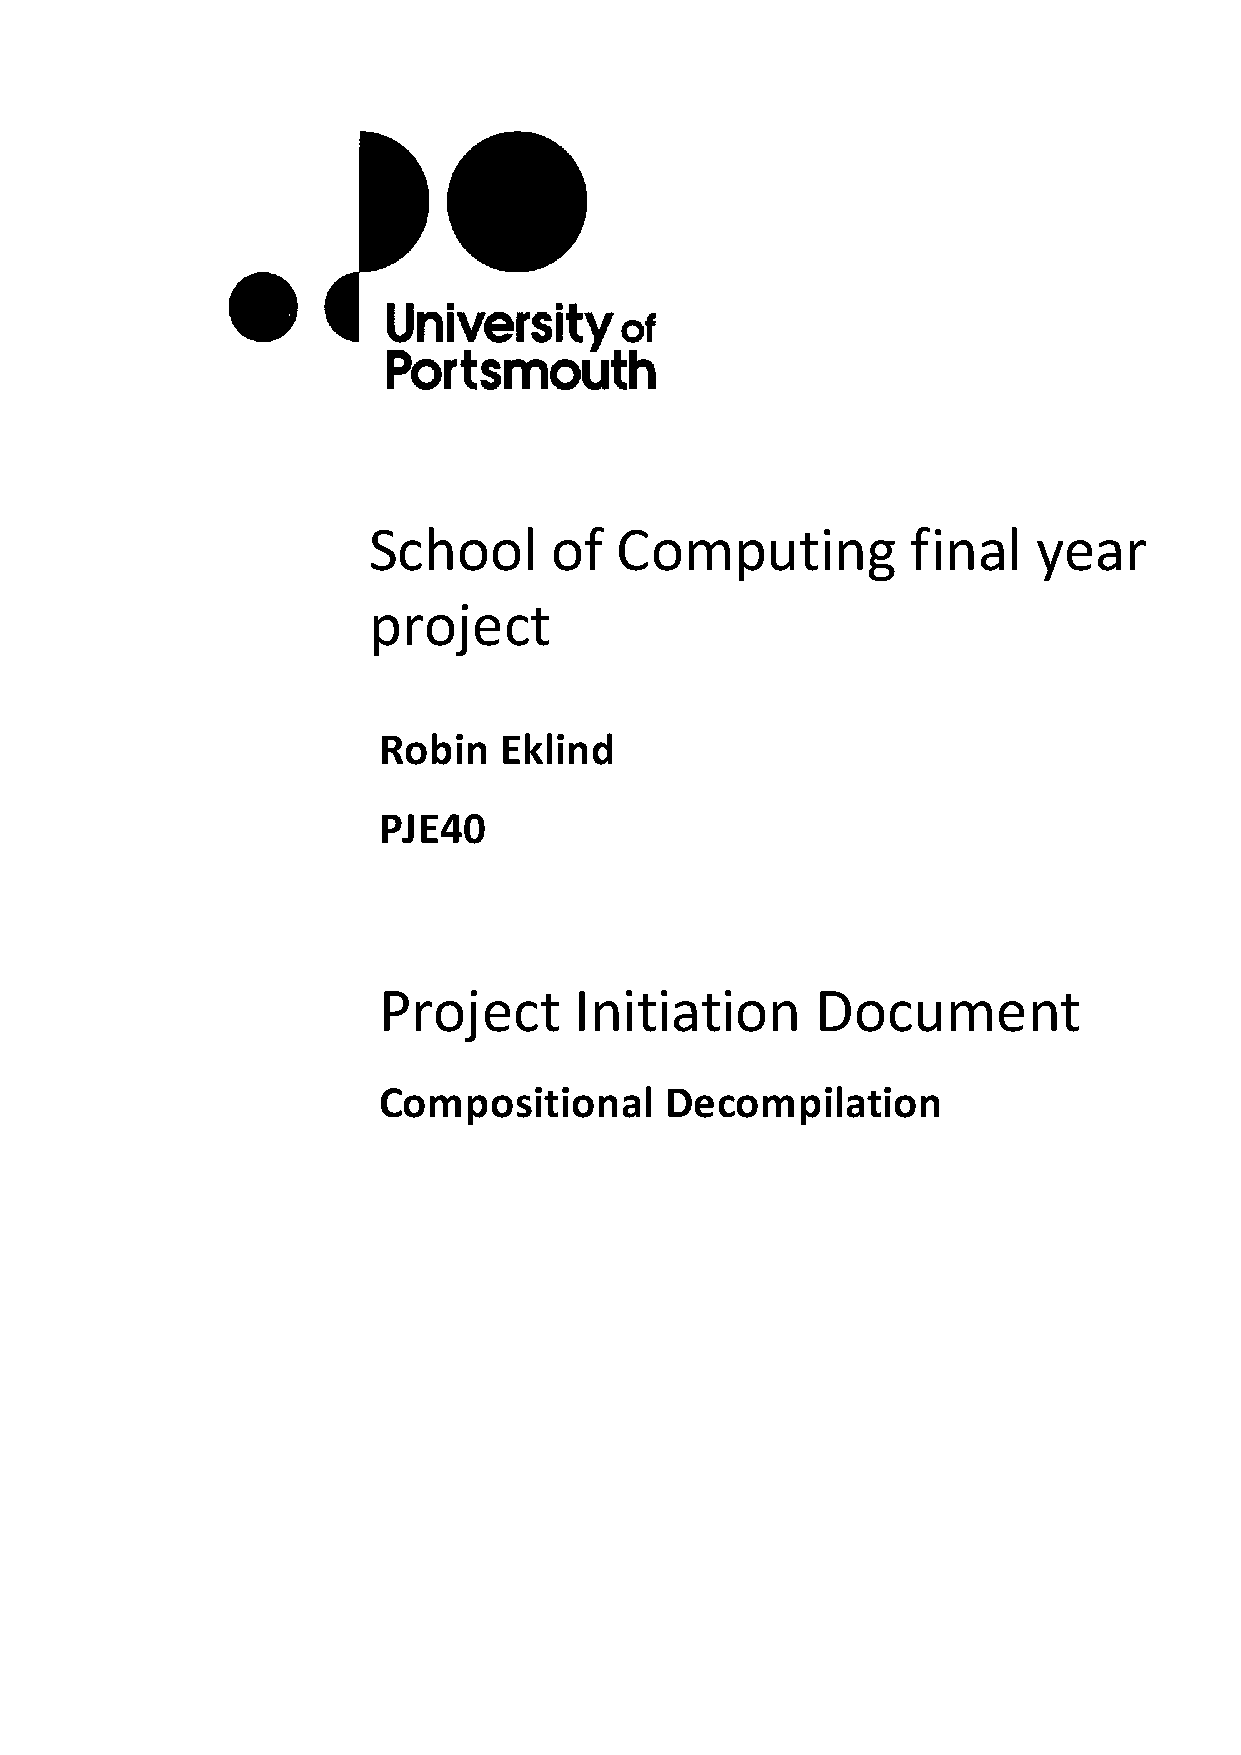
\includepdf[pages=-]{appendices/PID.pdf}

% --- [ Certificate of Ethics Review ] -----------------------------------------

\subsection{Certificate of Ethics Review}

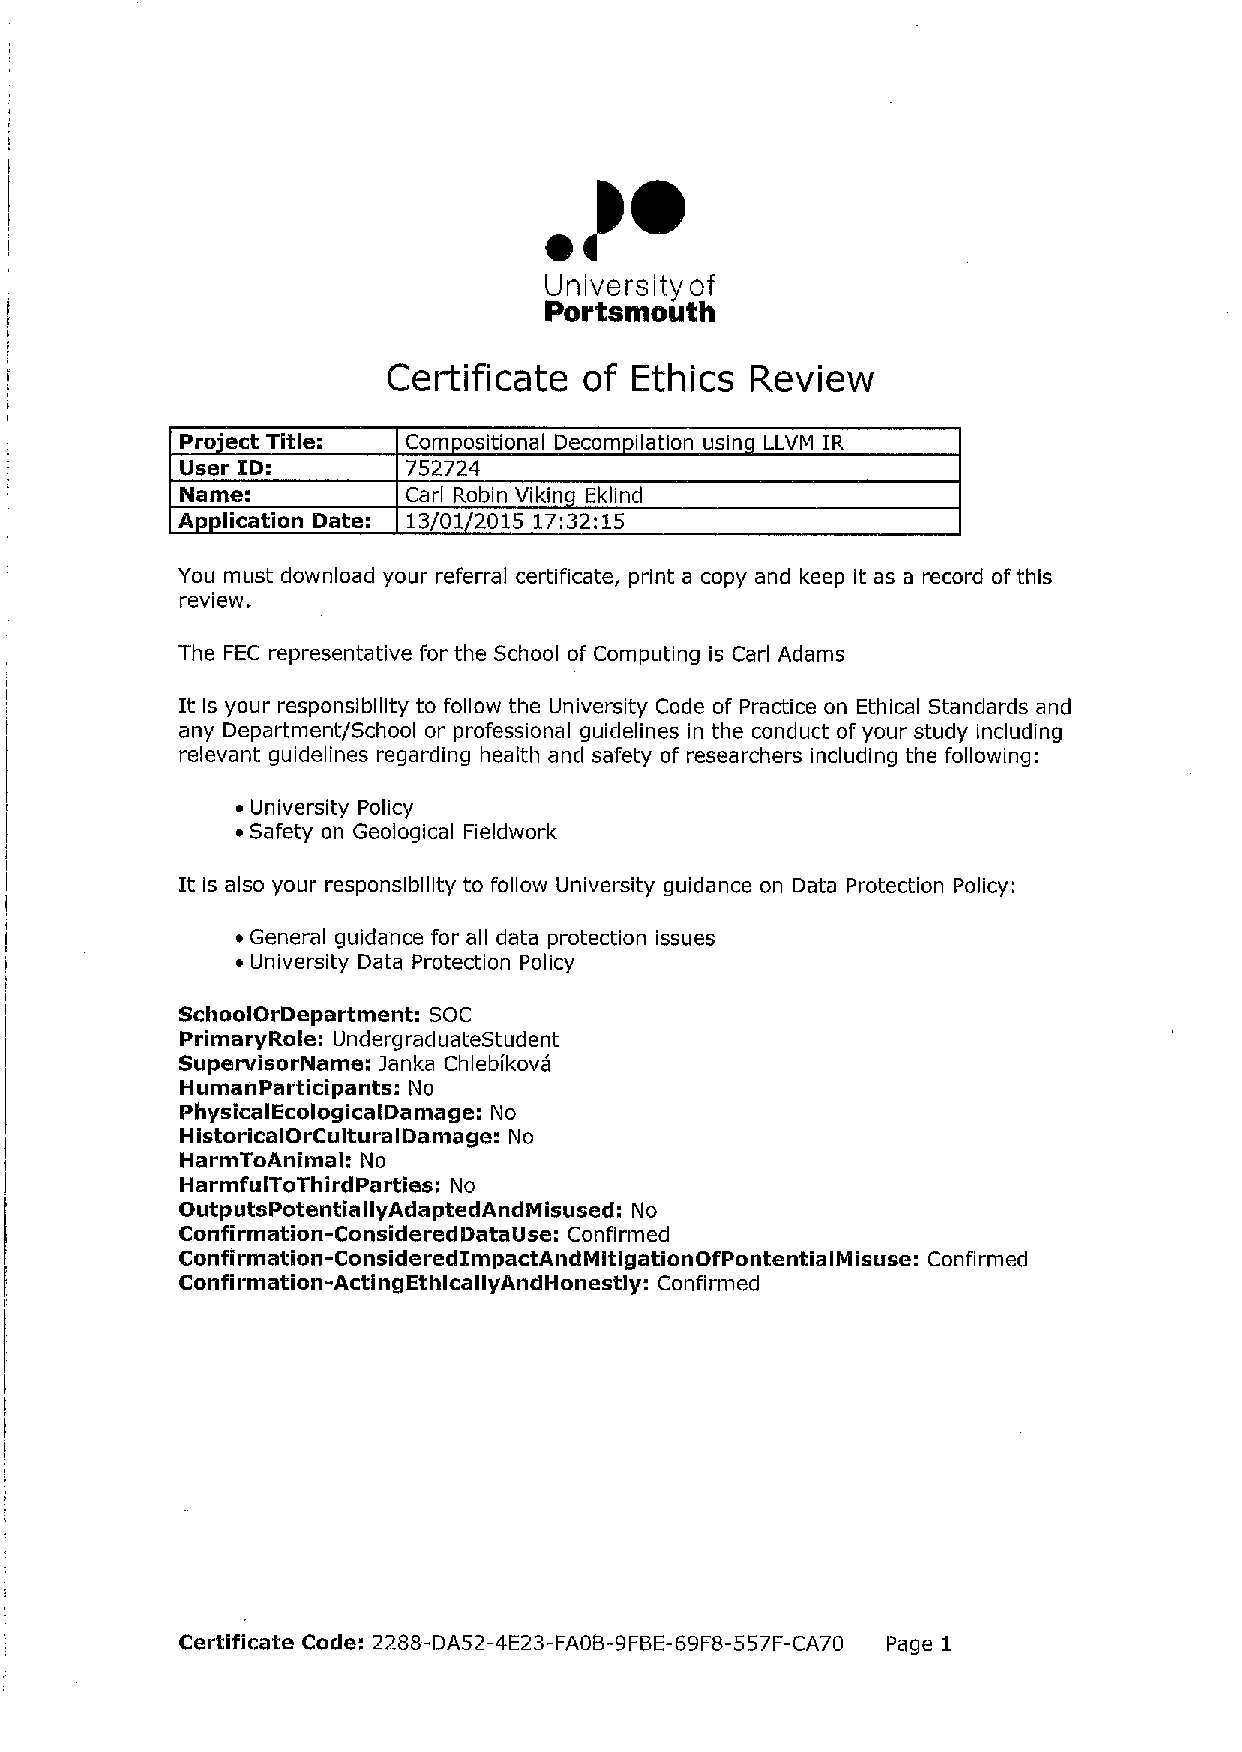
\includepdf[pages=-]{appendices/ethics_review.pdf}

% --- [ Gantt Chart ] ----------------------------------------------------------

\subsection{Initial and Final Gantt Charts}

\begin{figure}[htbp]
	\begin{center}
		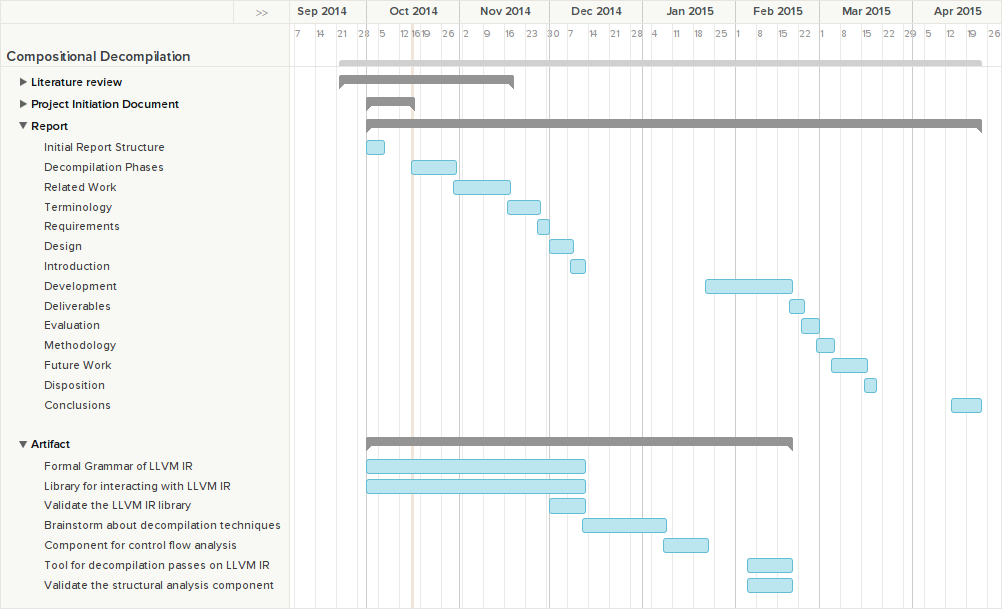
\includegraphics[angle=270, width=0.9\textwidth]{appendices/gantt_initial.png}
		\caption{Initial Gantt chart.}
	\end{center}
\end{figure}

% TODO: Add final Gantt chart.

\clearpage

% --- [ The REIL Instruction Set ] ---------------------------------------------

\subsection{The REIL Instruction Set}
\label{app:reil_instructions}

\lstinputlisting[language=reil, style=nasm, caption={A full definition of the REIL instruction set. \label{lst:reil_instructions}}]{appendices/reil_instruction_set.asm}

\clearpage

% --- [ Patch for Unnamed Basic Blocks of LLVM ] -------------------------------

\subsection{Patch for Unnamed Basic Blocks of LLVM}
\label{app:unnamed_patch}

The following patch ensures that the assembly printer of LLVM 3.6.0 always prints the generated names of unnamed basic blocks.

\lstinputlisting[language=diff, style=diff, caption={Always print the generated names of unnamed basic blocks. \label{lst:unnamed_patch}}]{appendices/unnamed.patch}

\clearpage

% --- [ Control Flow Analysis Example ] ----------------------------------------

\subsection{Control Flow Analysis Example}
\label{app:control_flow_analysis_example}

This section provides a step-by-step demonstration of how the control flow analysis is conducted by analysing the \texttt{stmt} function of the c4 compiler\footnote{C in four functions: \url{https://github.com/rswier/c4}}. The control flow analysis operates exclusively on CFGs, which are generated by a set of components prior to the control flow analysis stage. Firstly, the C source code of the c4 compiler is translated into LLVM IR by the Clang compiler of the front-end. Secondly, the LLVM IR is optionally optimized by the \texttt{opt} tool of the LLVM compiler framework. Lastly, a CFG is generated for each function of the LLVM IR using the \texttt{ll2dot} tool.

The control flow analysis stage uses subgraph isomorphism search algorithms to locate isomorphisms of the graph representations of high-level control flow primitives in the CFG of a given function, as further described in section \ref{sec:design_control_flow_analysis}. The CFG is simplified by recursively replacing the identified subgraphs with single nodes until the entire CFG has been reduced into a single node. By recoding the node names of the identified subgraph isomorphisms and the name of their corresponding high-level control flow primitives, a structured CFG may be produced in which all nodes are known to belong to a high-level control flow primitive.

The pseudo-code and graph representations of the supported high-level control flow primitives are presented in figure \ref{fig:graph_representations} of section \ref{sec:control_flow_analysis}. Should the control flow analysis fail to reduce a CFG into a single node, the CFG is considered irreducible with regards to the supported high-level control flow primitives; in which case a structured CFG cannot be produced.

For this demonstration, the CFG of the \texttt{stmt} function is the starting point of the control flow analysis stage. The first step of the control flow analysis recursively locates subgraph isomorphisms of the graph representation of pre-test loops (see figure \ref{fig:pre_test_graph_representation}) in the original CFG of the \texttt{stmt} function, and replaces these subgraphs with single nodes as illustrated in figure \ref{fig:step_1}.

\begin{figure}[htbp]
	\centering
	\begin{subfigure}[t]{0.45\textwidth}
		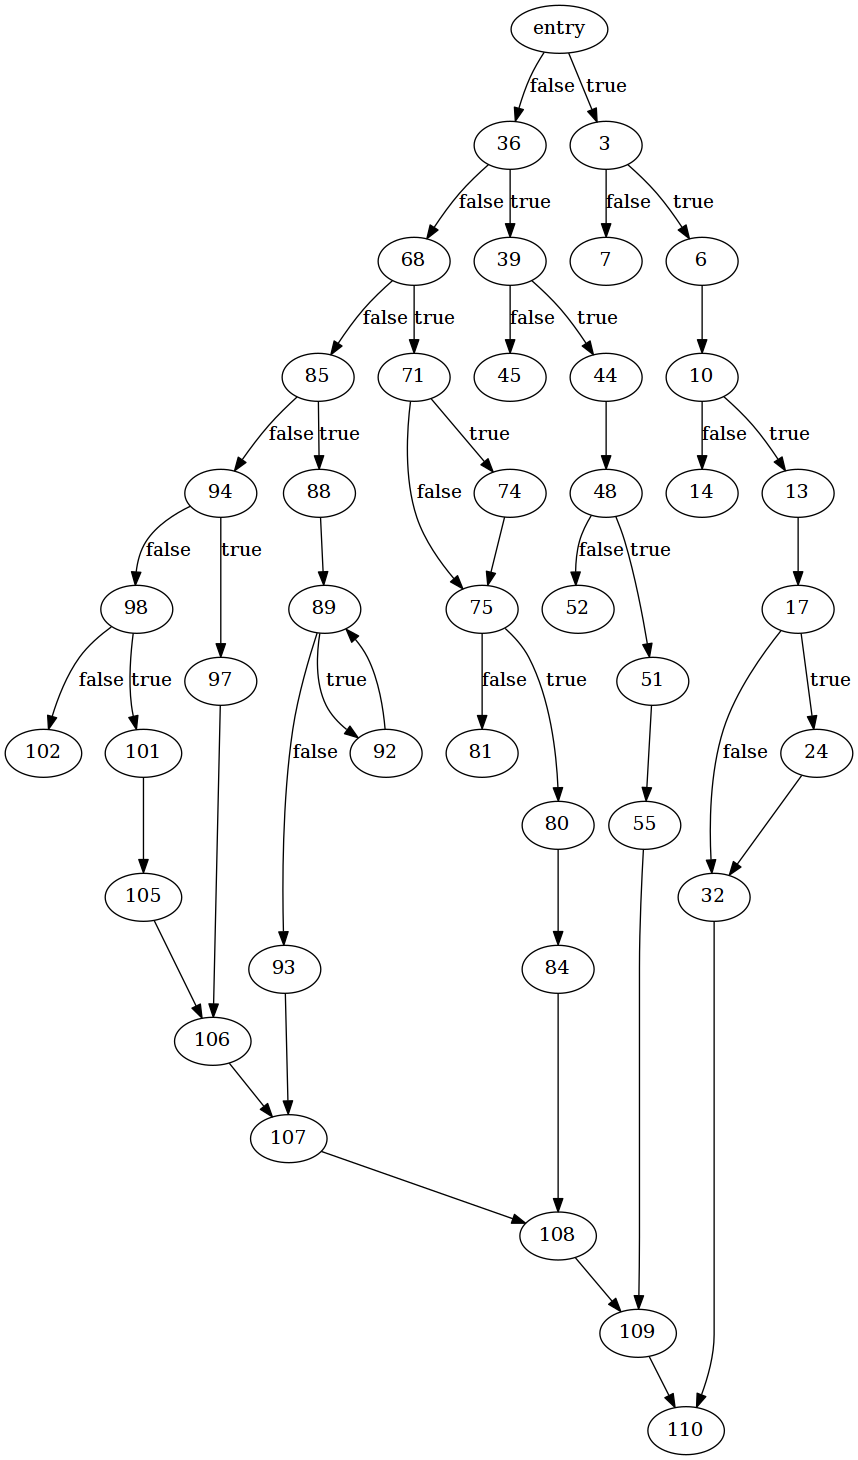
\includegraphics[width=\textwidth]{appendices/stmt_example/stmt_0.png}
	\end{subfigure}
	\qquad
	\begin{subfigure}[t]{0.45\textwidth}
		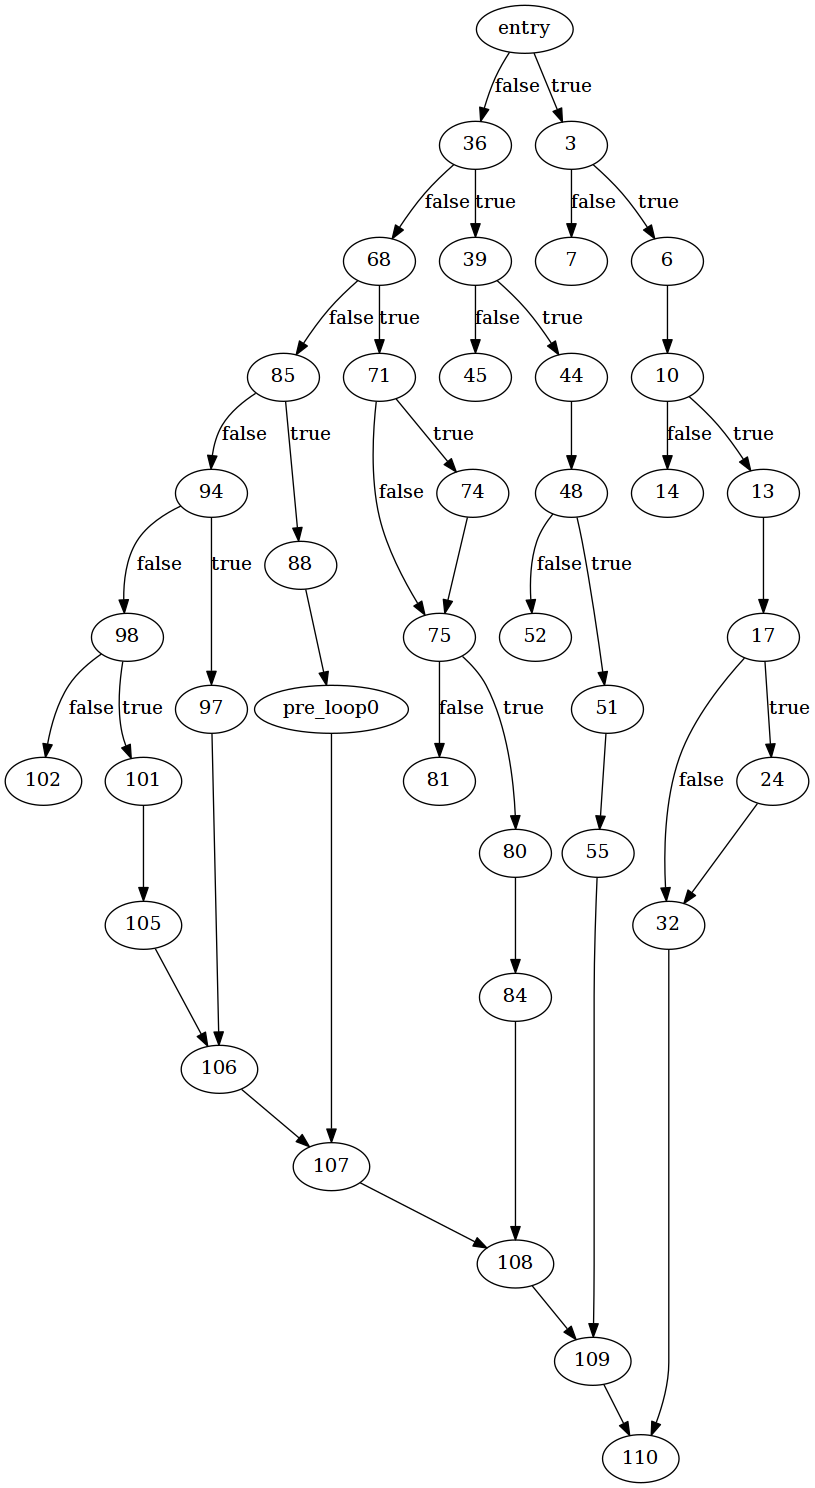
\includegraphics[width=\textwidth]{appendices/stmt_example/stmt_1.png}
	\end{subfigure}
	\caption{\textbf{Step 1}. The original CFG of the \texttt{stmt} function (left) and a simplified CFG (right) after identifying pre-test loops (see figure \ref{fig:pre_test_graph_representation}).}
	\label{fig:step_1}
\end{figure}

The second step further simplifies the CFG of \textbf{step 1} by recursively replacing the subgraph isomorphisms of the graph representation of consecutive statements (see figure \ref{fig:list_graph_representation}) with single nodes, as illustrated in figure \ref{fig:step_2}.

\begin{figure}[htbp]
	\centering
	\begin{subfigure}[t]{0.45\textwidth}
		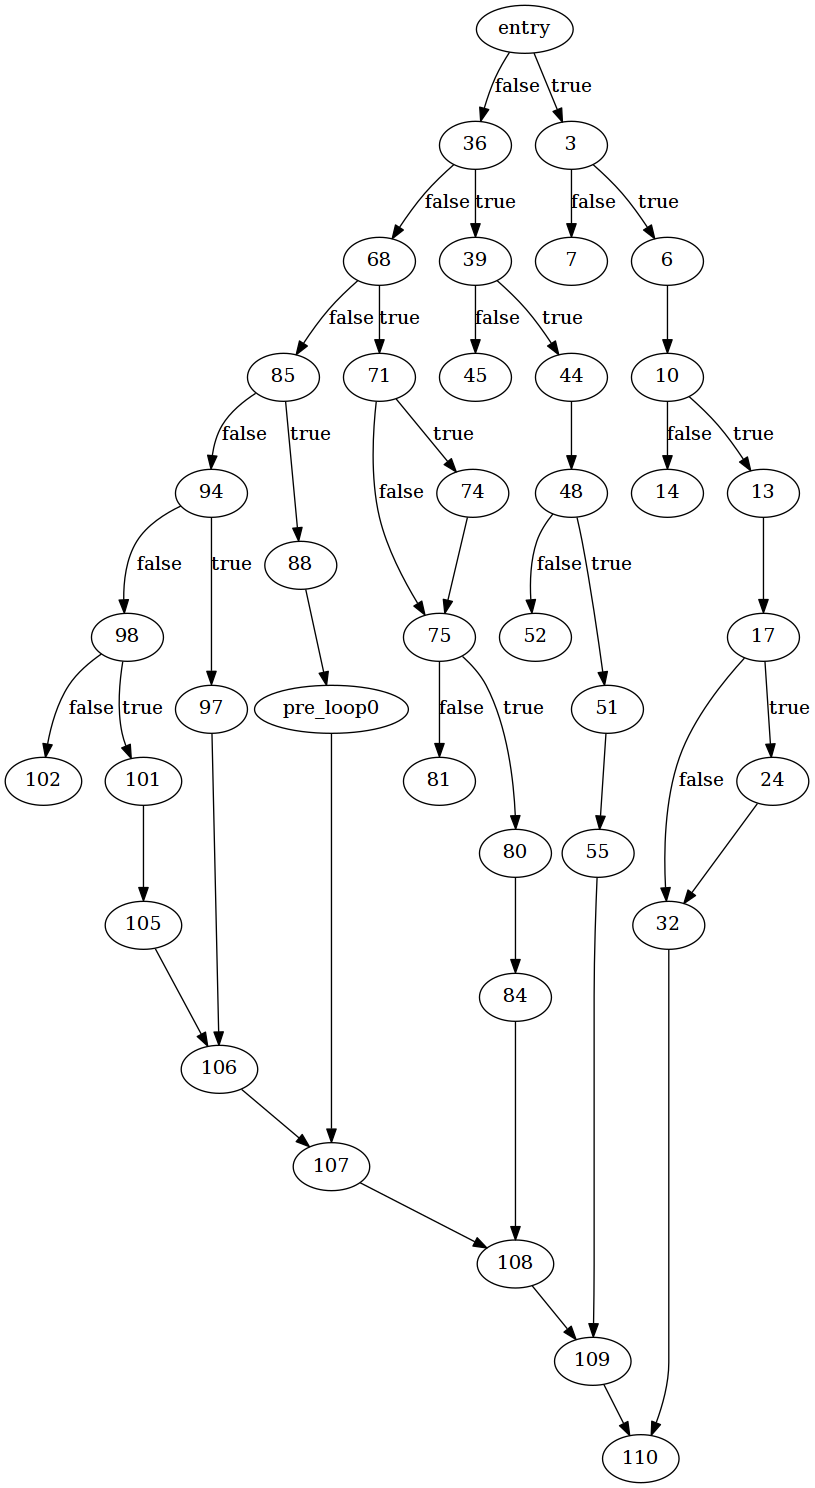
\includegraphics[width=\textwidth]{appendices/stmt_example/stmt_1.png}
	\end{subfigure}
	\qquad
	\begin{subfigure}[t]{0.45\textwidth}
		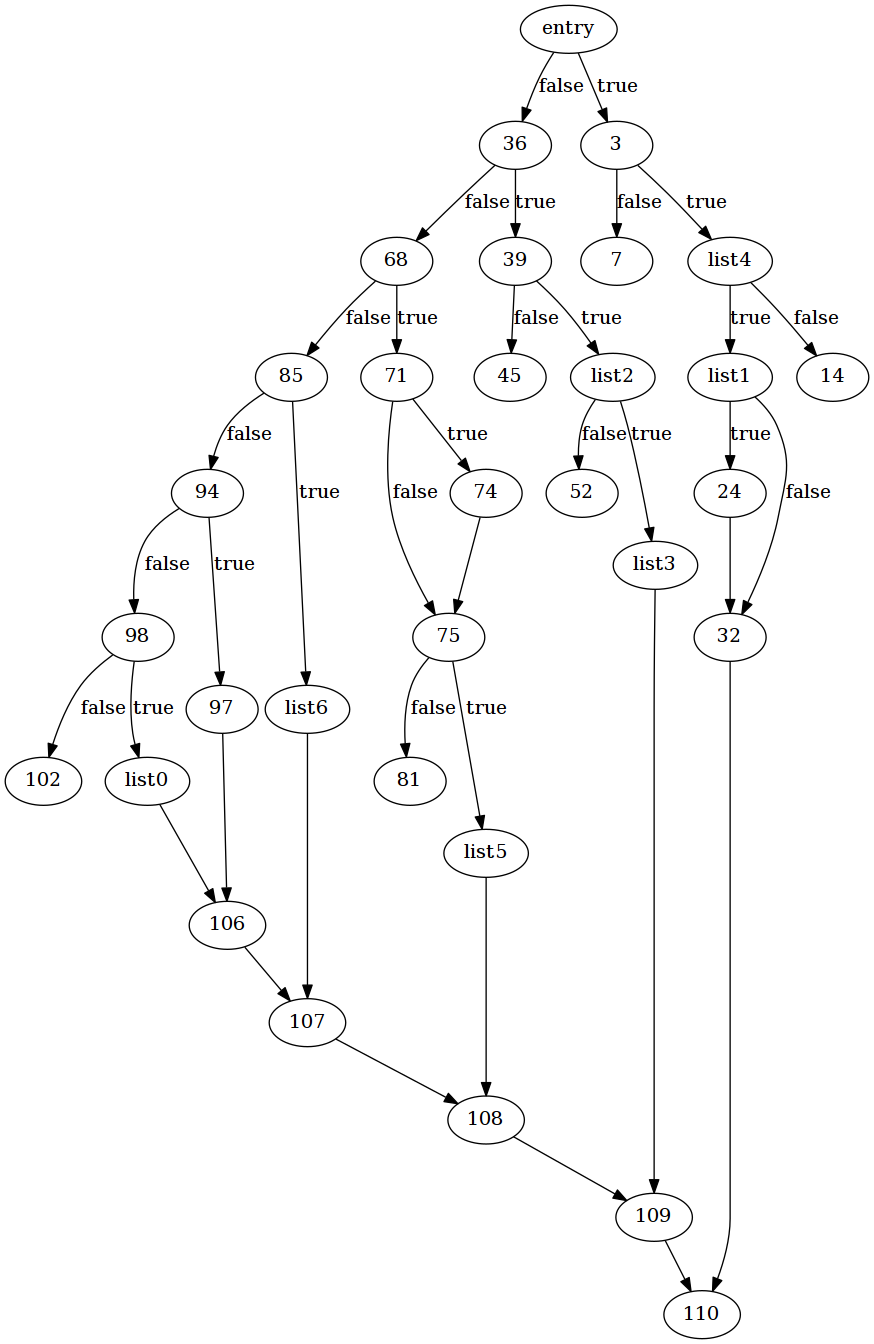
\includegraphics[width=\textwidth]{appendices/stmt_example/stmt_2.png}
	\end{subfigure}
	\caption{\textbf{Step 2}. The CFG from \textbf{step 1} (left) and a simplified CFG (right) after identifying consecutive statements (see figure \ref{fig:list_graph_representation}).}
	\label{fig:step_2}
\end{figure}

The third step further simplifies the CFG of \textbf{step 2} by recursively replacing the subgraph isomorphisms of the graph representation of 1-way conditionals (see figure \ref{fig:if_graph_representation}) with single nodes, as illustrated in figure \ref{fig:step_3}.

\begin{figure}[htbp]
	\centering
	\begin{subfigure}[t]{0.45\textwidth}
		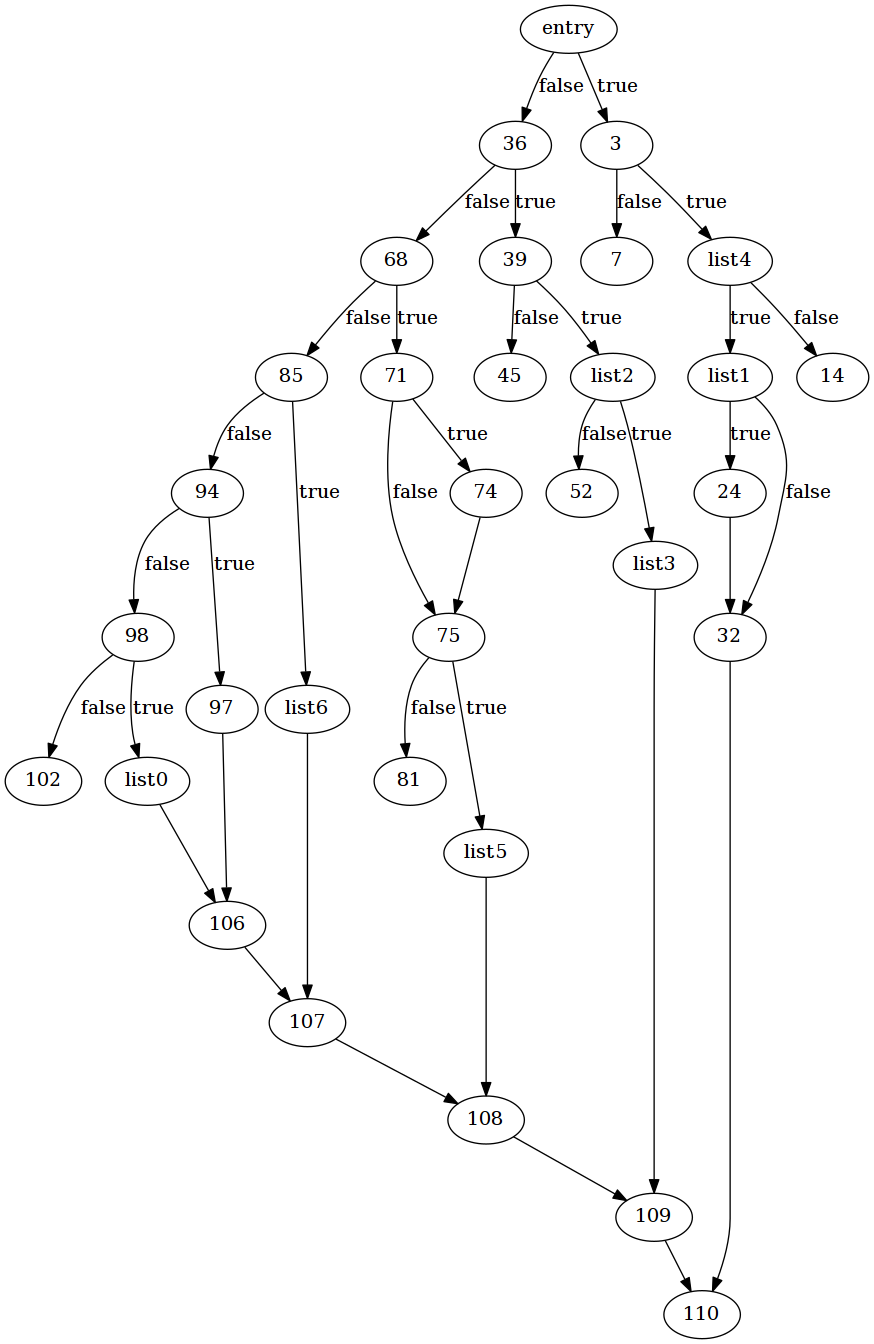
\includegraphics[width=\textwidth]{appendices/stmt_example/stmt_2.png}
	\end{subfigure}
	\qquad
	\begin{subfigure}[t]{0.45\textwidth}
		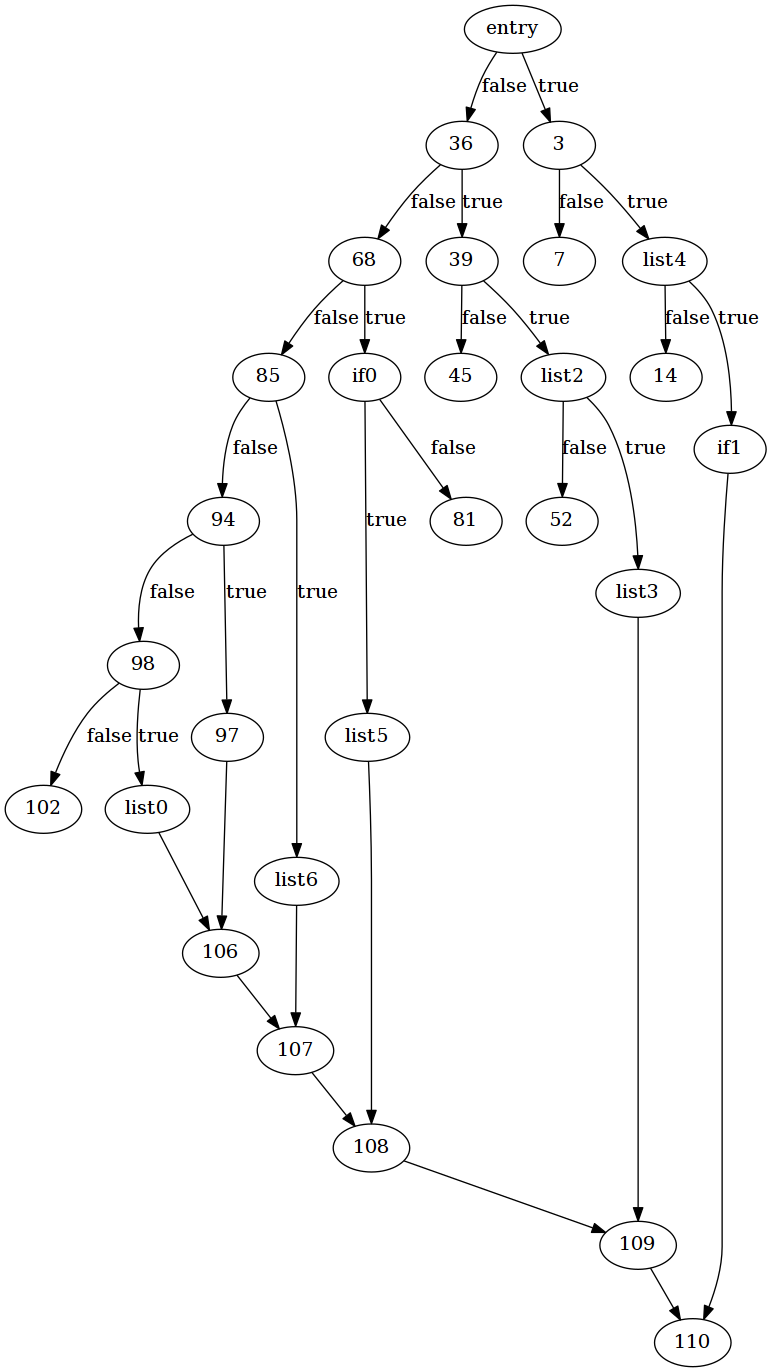
\includegraphics[width=\textwidth]{appendices/stmt_example/stmt_3.png}
	\end{subfigure}
	\caption{\textbf{Step 3}. The CFG from \textbf{step 2} (left) and a simplified CFG (right) after identifying 1-way conditionals (see figure \ref{fig:if_graph_representation}).}
	\label{fig:step_3}
\end{figure}

The fourth step further simplifies the CFG of \textbf{step 3} by recursively replacing the subgraph isomorphisms of the graph representation of 1-way conditionals with body return statements (see figure \ref{fig:if_return_graph_representation}) with single nodes, as illustrated in figure \ref{fig:step_4}.

\begin{figure}[htbp]
	\centering
	\begin{subfigure}[t]{0.45\textwidth}
		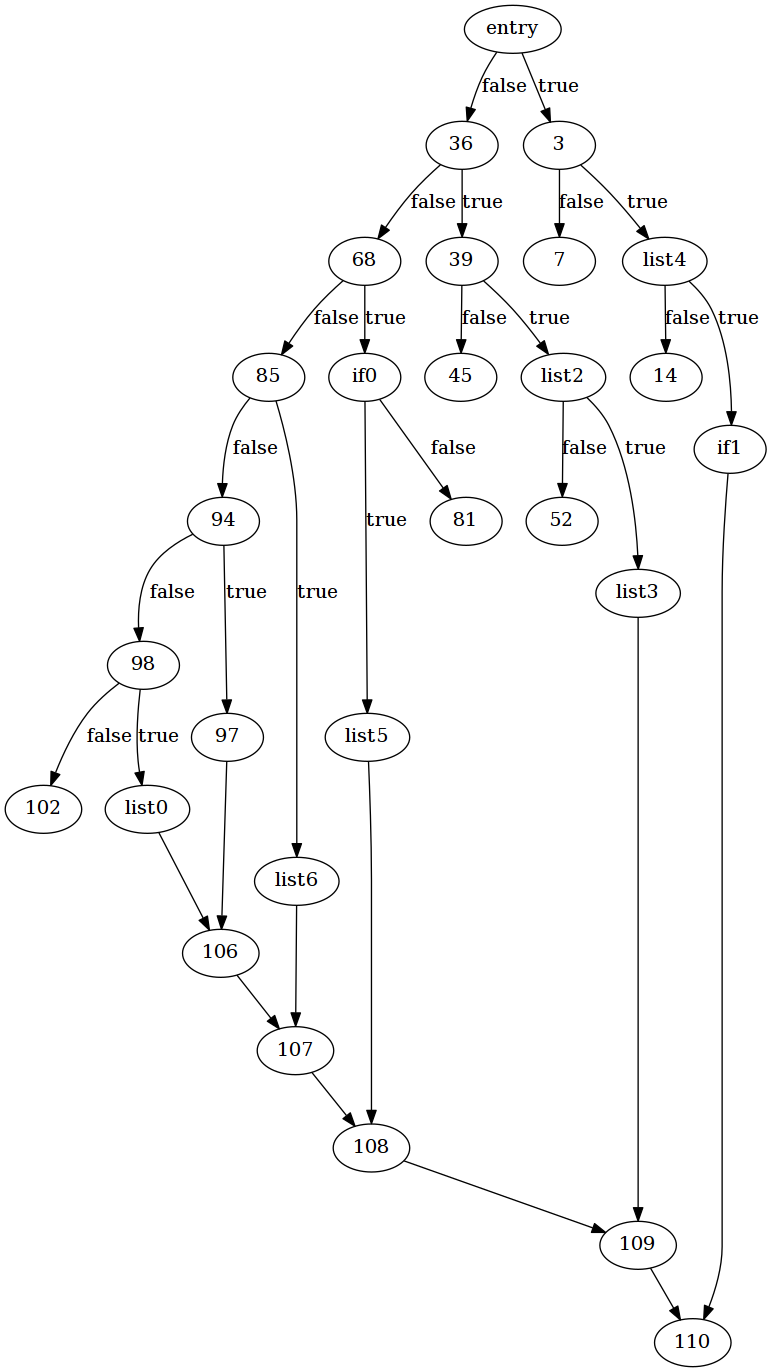
\includegraphics[width=\textwidth]{appendices/stmt_example/stmt_3.png}
	\end{subfigure}
	\qquad
	\begin{subfigure}[t]{0.45\textwidth}
		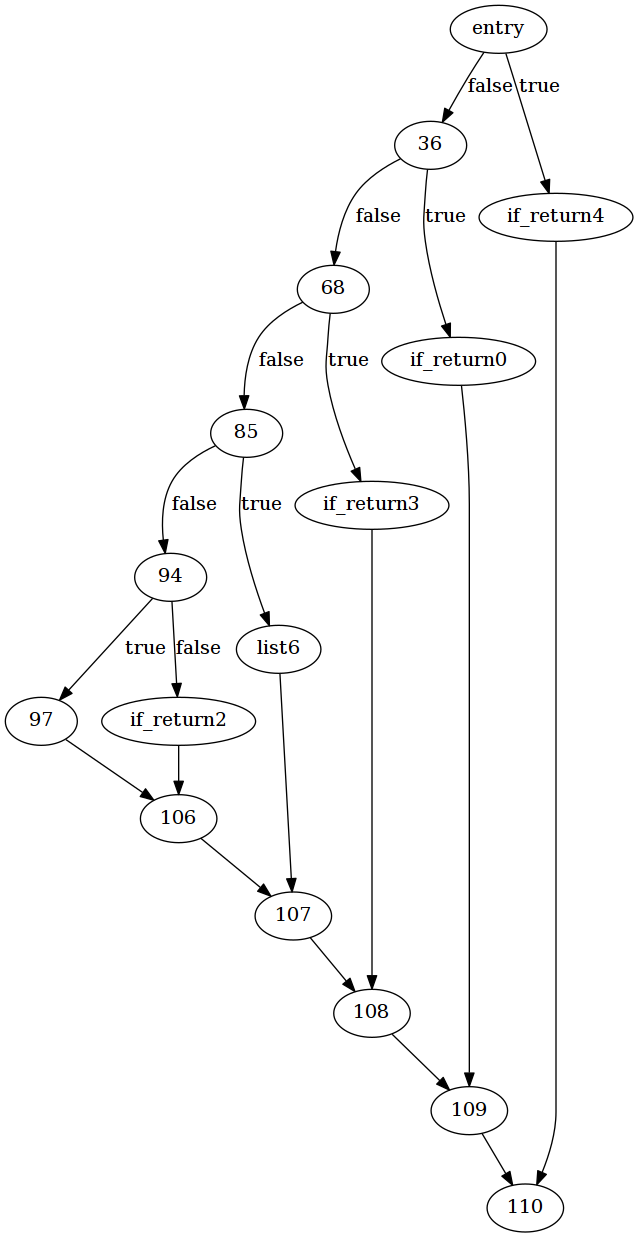
\includegraphics[width=\textwidth]{appendices/stmt_example/stmt_4.png}
	\end{subfigure}
	\caption{\textbf{Step 4}. The CFG from \textbf{step 3} (left) and a simplified CFG (right) after identifying 1-way conditionals with body return statements (see figure \ref{fig:if_return_graph_representation}).}
	\label{fig:step_4}
\end{figure}

The last step of the control flow analysis stage reduces the CFG of \textbf{step 4} into a single node by recursively replacing the subgraph isomorphisms of the graph representation of 2-way conditionals (see figure \ref{fig:if_else_graph_representation}) with single nodes, as illustrated in figure \ref{fig:step_5}.

\begin{figure}[htbp]
	\centering
	\begin{subfigure}[t]{0.45\textwidth}
		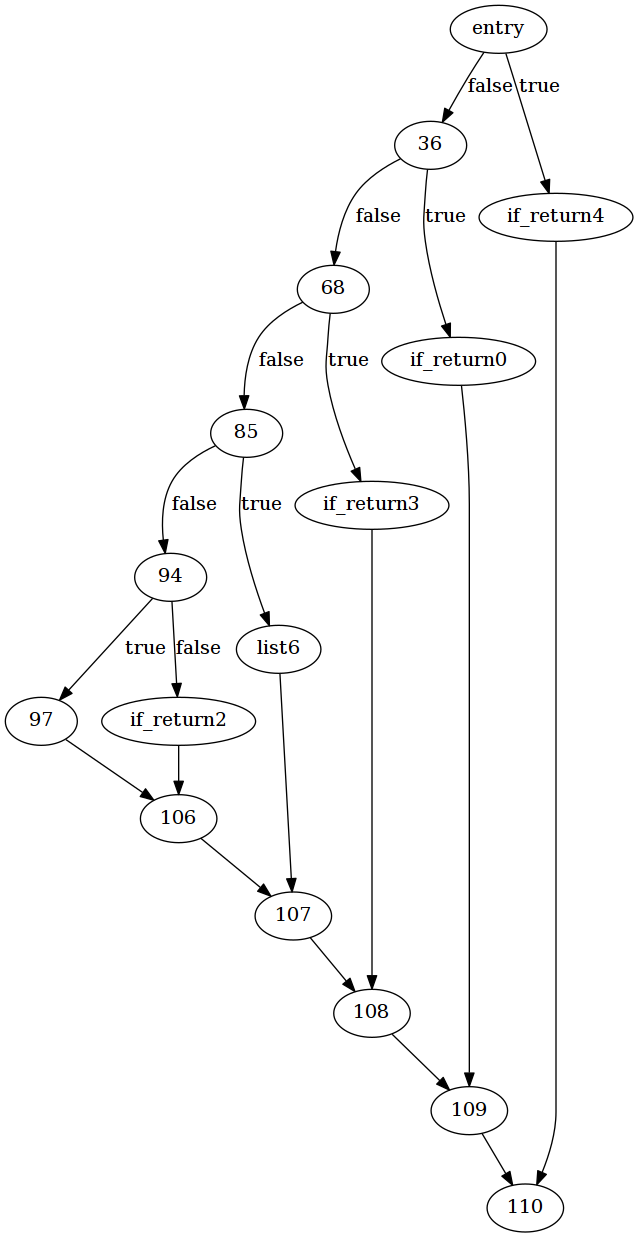
\includegraphics[width=\textwidth]{appendices/stmt_example/stmt_4.png}
	\end{subfigure}
	\qquad
	\begin{subfigure}[t]{0.45\textwidth}
		\centering
		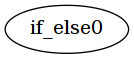
\includegraphics[width=0.3\textwidth]{appendices/stmt_example/stmt_5.png}
	\end{subfigure}
	\caption{\textbf{Step 5}. The CFG from \textbf{step 4} (left) and a simplified CFG (right) after identifying 2-way conditionals (see figure \ref{fig:if_else_graph_representation}).}
	\label{fig:step_5}
\end{figure}

\clearpage

% --- [ Restructure Example ] --------------------------------------------------

\subsection{Restructure Example}
\label{app:restructure_example}

The \texttt{restructure} tool produces structured CFGs (in JSON format) from unstructured CFGs (in the DOT file format), as described in section \ref{sec:impl_control_flow_analysis_tool}. Listing \ref{lst:restructure_output} demonstrates the output of the restructure tool when analysing the CFG of the \texttt{stmt} function of the c4 compiler, which is presented on the left side of figure \ref{fig:step_1}.

\lstinputlisting[language=go, style=go, caption={The structured control flow graph (in JSON format) produced by the \texttt{restructure} tool when analysing the CFG of the \texttt{stmt} function of the c4 compiler. \label{lst:restructure_output}}]{appendices/stmt_example/stmt.json}

\clearpage

% --- [ Post-processing Example ] ----------------------------------------------

\subsection{Post-processing Example}

foo

% unresolved
\begin{figure}[htbp]
	\centering
	\begin{subfigure}[t]{0.45\textwidth}
		\lstinputlisting[language=go, style=go]{appendices/post_example/foo_0.go}
	\end{subfigure}
	\qquad
	\begin{subfigure}[t]{0.45\textwidth}
		\lstinputlisting[language=go, style=go]{appendices/post_example/foo_1.go}
	\end{subfigure}
	\caption{foo}
	\label{fig:foo}
\end{figure}

foo

% mainret
\begin{figure}[htbp]
	\centering
	\begin{subfigure}[t]{0.45\textwidth}
		\lstinputlisting[language=go, style=go]{appendices/post_example/foo_1.go}
	\end{subfigure}
	\qquad
	\begin{subfigure}[t]{0.45\textwidth}
		\lstinputlisting[language=go, style=go]{appendices/post_example/foo_2.go}
	\end{subfigure}
	\caption{foo}
	\label{fig:foo}
\end{figure}

foo

% localid
\begin{figure}[htbp]
	\centering
	\begin{subfigure}[t]{0.45\textwidth}
		\lstinputlisting[language=go, style=go]{appendices/post_example/foo_2.go}
	\end{subfigure}
	\qquad
	\begin{subfigure}[t]{0.45\textwidth}
		\lstinputlisting[language=go, style=go]{appendices/post_example/foo_3.go}
	\end{subfigure}
	\caption{foo}
	\label{fig:foo}
\end{figure}

foo

% assignbinop
\begin{figure}[htbp]
	\centering
	\begin{subfigure}[t]{0.45\textwidth}
		\lstinputlisting[language=go, style=go]{appendices/post_example/foo_3.go}
	\end{subfigure}
	\qquad
	\begin{subfigure}[t]{0.45\textwidth}
		\lstinputlisting[language=go, style=go]{appendices/post_example/foo_4.go}
	\end{subfigure}
	\caption{foo}
	\label{fig:foo}
\end{figure}

foo

% deadassign
\begin{figure}[htbp]
	\centering
	\begin{subfigure}[t]{0.45\textwidth}
		\lstinputlisting[language=go, style=go]{appendices/post_example/foo_4.go}
	\end{subfigure}
	\qquad
	\begin{subfigure}[t]{0.45\textwidth}
		\lstinputlisting[language=go, style=go]{appendices/post_example/foo_5.go}
	\end{subfigure}
	\caption{foo}
	\label{fig:foo}
\end{figure}

foo

% forloop
\begin{figure}[htbp]
	\centering
	\begin{subfigure}[t]{0.45\textwidth}
		\lstinputlisting[language=go, style=go]{appendices/post_example/foo_5.go}
	\end{subfigure}
	\qquad
	\begin{subfigure}[t]{0.45\textwidth}
		\lstinputlisting[language=go, style=go]{appendices/post_example/foo_6.go}
	\end{subfigure}
	\caption{foo}
	\label{fig:foo}
\end{figure}


\end{document}
